\documentclass[a4paper,10pt]{article} % Artikel med 12pt text och A4 storlek.
%\documentclass[draft,10pt]{article} % Artikel med 12pt text och A4 storlek.
\usepackage[english]{babel} % Svensk avstavning istället för engelsk
%\usepackage[pdflatex]{graphicx}% De här två behövs för svenska
\usepackage[utf8]{inputenc} % UTF-8 encodad fil. Kan bytas ut mot latin1 om en vill...
\usepackage[T1]{fontenc}
\usepackage[authoryear]{natbib}
\usepackage{bibentry}
\usepackage{subcaption}
\usepackage{boldline} 
%\usepackage[allfiguresdraft]{draftfigure}
\usepackage{float}
\usepackage[margin=2.5cm]{geometry}
\usepackage{setspace}
\usepackage{color}
\usepackage{enumitem}   
\usepackage[T1]{tipa}
\usepackage{tabu}
\usepackage{textcomp}
\usepackage{rotating}
\usepackage{booktabs}
\renewcommand{\arraystretch}{1.3}
\usepackage{tabu}

\usepackage{longtable}
\usepackage{pbox}
\usepackage{setspace}
\usepackage{lscape}
%\usepackage{enumitem}
%\usepackage{enumerate}
\setcounter{secnumdepth}{4}
\setcounter{tocdepth}{5}
\usepackage{array}
\newcolumntype{?}{!{\vrule width 1pt}}
\newcolumntype{L}[1]{>{\raggedright\let\newline\\\arraybackslash\hspace{0pt}}m{#1}}
\newcolumntype{C}[1]{>{\centering\let\newline\\\arraybackslash\hspace{0pt}}m{#1}}
\newcolumntype{R}[1]{>{\raggedleft\let\newline\\\arraybackslash\hspace{0pt}}m{#1}}
%\usepackage{graphics}
\usepackage{graphicx}
\usepackage{subcaption}

\usepackage{lipsum}



\usepackage{footnote}
\usepackage{tipx}

\usepackage{wrapfig}
\usepackage[table,dvipsnames]{xcolor}
\usepackage{multirow}

\usepackage{titlesec}

\setcounter{secnumdepth}{4}


\usepackage{color}  
\usepackage{hyperref}
\hypersetup{
    colorlinks=true, %set true if you want colored links
    linktoc=all,     %set to all if you want both sections and subsections linked
    linkcolor=violet,  %choose some color if you want links to stand out
            urlcolor=blue,
            citecolor=Thistle,
}

\usepackage{xcolor}

\definecolor{hedvig_blue}{HTML}{7D81F5}
\definecolor{hedvig_lightgreen}{HTML}{81F093}
\definecolor{hedvig_darkgreen}{HTML}{0B8C1F}
\definecolor{hedvig_orange}{HTML}{FFB87A}
\definecolor{hedvig_red}{HTML}{FFD9E0}
\definecolor{hedvig_yellow}{HTML}{FCFFA8}



\setcitestyle{notesep={:},aysep={},aasep={\&}}
%\renewcommand{\labelitemi}{$\rightarrow$}
\usepackage{gb4e}

%\usepackage{draftwatermark}
%\SetWatermarkText{DRAFT}
%\SetWatermarkScale{4}

%\pagestyle{myheadings}

\noautomath
\title{Predicting number of languages per island group in Remote Oceania}
%\large A thesis submitted for the degree of Doctor of Philosophy of The Australian National University\\}

\author{anon}
%\author{Hedvig Skirg{\aa}rd}
\setlength{\parindent}{0pt}
\setlength{\parskip}{1ex plus 0.5ex minus 0.2ex}

\begin{document}
\def\code#1{\texttt{#1}}

\thispagestyle{empty}
%\singlespacing

\maketitle
\thispagestyle{empty}

\newpage



\newpage
\singlespacing
\tableofcontents

\newpage
\listoffigures
 \listoftables
 \vspace{0.7cm}


\newpage
\pagenumbering{arabic}

%%toberemoved %\doublespacing


\newpage

\section{Predicting language diversity in Remote Oceania}
\label{chapter_pol_complex}
\subsection{Introduction}
\doublespacing
%\doublespacing
Why are there more languages in some places than others? The number of languages of the world are not equally distributed over its population. In Papua New Guinea, there are 835 languages for a population of 7 million people \citep{ethnologue22, cia_world_factbook_2019}. However, in South Korea there are only two indigenous spoken languages in a population of 51 million people. The function of language is the same across the world, so how could this be?

Understanding the mechanics of language change and diversification is essential to understanding human history. It is the story of how languages, and therefore also communities, become separated from each other. This research topic has received a lot of attention in recent years (c.f. \citet{gavin2017process,  greenhill2015demographic, Pacheco_Coelho_2019, hua2019ecological}), and in this chapter we will take a closer look at Remote Oceania. 

Fig.~\ref{RO_overnight_coloured_dots} shows islands of Oceania. Languages are points, coloured by language family. In the Polynesian islands (S\={a}moa, Tonga, Rarotonga, Tokelau etc) there is generally one language per island group. However, Melanesian Remote Oceania (Vanuatu, Temotu, Fiji and Kanaky (New Caledonia)) have many more languages, sometimes up to 20 languages on the very same island. What explains this difference?
%What are the mechanics of this?



\begin{sidewaysfigure}[p]
\centering
\includegraphics[width=19cm]{illustrations/CartoGIS_oceania_languages_subgreions_edited.png}
\caption{}
\label{RO_overnight_coloured_dots}
\end{sidewaysfigure}



% grouped by overnight sailing distances \citep{mark_1986, marck2000}


%\footnote{Lines separating Near and Remote Oceania added on by me.}


Diversification takes time. We would expect a higher probability of language diversification in areas where people have lived for a longer time simply due to natural drift as communities spread out and form separate clusters. A large part of Remote Oceania was settled for the first time by Austronesian speaking people in a rapid expansion 3,600 - 2,800 BP known as the ``Lapita expansion'' (\citet[106-7]{bellwood2006austronesians}; \citet[137]{rieth_cochrane_2018}). This area covers all islands of Vanuatu, Temotu, New Caledonia, Fiji and parts of Western Polynesia. These dates of first settlement for these islands are relatively similar, but there still is a large discrepancy in number of languages. This makes for a natural experiment which we can use to test hypotheses about language diversification.

Let us compare two islands in this region as an example: S\={a}moa in Western Polynesia and Malakula in Vanuatu. S\={a}moa was settled approximately 400 years after Malakula  \citep[137-8]{rieth_cochrane_2018}, a relatively short span of time with respect to language diversification. Besides time depth, we might also expect that greater land mass entails greater language diversity. A larger area promotes increased population spread, leading to language isolation. The shoreline\footnote{Since Austronesian settlements are mainly found on the coast, we are comparing shorelines instead of land area in this example. The data of this chapter contains information on land area, land area + water; and shoreline.} of Malakula is 67\% of that of S\={a}moa. Given these two facts and our assumptions, we might expect S\={a}moa and Malakula to have similar numbers of languages, or perhaps even that Malakula has fewer. However, S\={a}moa sports \emph{one} indigenous language and Malakula has \emph{thirty-three} \citep{glottolog40}. Why is this?

%\citet{Pacheco_Coelho_2019} and \citet[119]{lynchrosscrowleyinternalsubgroupingoceanic} 

\citet{turner1884} and \citet{pawley81,pawley2007} have suggested that the discrepancy between the number of languages in different parts of Remote Oceania can be related to societal structure. Societies in Melanesian Remote Oceania tend to be less hierarchical than societies in Western Polynesia, and societies with fewer vertical levels of political structures are associated with more linguistic and cultural diversity. Conversely, more hierarchically complex societies are associated with linguistic and cultural homogeneity. This hypothesis does not necessarily entail that individual leaders in more stratified societies have a direct effect on the nature of the language of the community by means of their personality, conscious policies or directives. Instead, it is more likely that the political structure is indicative of different kinds of community network structures and attitudes. A measurement of so-called ``political complexity'' in ethnographic surveys (c.f. \citet{gray1998ethnographic}) should then be correlated with different patterns of interaction and show up as a significant factor in language diversification. This is true even if political complexity is merely a proxy measurement of the interaction pattern that is in fact driving language change. 

This chapter tests this hypothesis by constructing a model where we try to predict the number of languages per island group using data on \textit{settlement time}, \textit{environment} and \textit{political complexity}. Environmental factors are included because it has been suggested that they are also drivers of language diversity (c.f. \citet{NETTLE1998}, \citet{gavin2012island} and \citet{hua2019ecological}). If the results show that political complexity has a significant correlation with the number of languages per island group when other relevant factors are controlled for, this lends support to Turner and Pawley's hypothesis.
 
%We will be using cultural data on societal structures in societies of Remote Oceania, archaeological dates and environmental variables (temperature and rainfall) to test if the political structure still significantly predicts the number of languages once other factors have been taken into account. Fig.~\ref{RO_overnight_coloured_dots} shows languages in Oceania, with islands grouped by overnight sailing distances \citep{mark_1986, marck2000}. In this study, we are concerned with languages of Remote Oceania (see Fig.~\ref{Remote_Oceania_subregions} for subregions of Oceania), and in particular Vanuatu and New Caledonia compared to the rest.

%First, we will go through previous research, secondly, we will have an overview of the region given the variables we are using in the study. Thirdly, the method will be presented and lastly we will go through the results and possible interpretations of them.

 
 
\subsection{Previous research}
\label{nonlingfactors}
Linguists, anthropologists and scholars of other fields have long remarked on the link between linguistic diversity and political structure in Remote Oceania. One of the oldest examples of this observation is Turner who travelled in the region 1861-1884 and hypothesised that the lack of regional variation within S\={a}moan entailed that they had long had a more centralised government \citep[172]{turner1884}.

%\begin{quotation} 
%\noindent \emph{To anyone acquainted with the aborigines of various parts of the world, and especially those of the Papuan groups in Western Polynesia [sic], the simple fact that S\={a}moans had but one dialect, and free intercourse with each other all over the group is proof positive that there must have long existed there some system of government.} \citep[172]{turner1884}\footnote{\citet[8]{moselhovdhaugen1992} in their reference grammar of Samoan also propose that the lack of regional diversity within the language is due to the extensive social networks and linking of different regions. More on this in chapter \ref{chapter_samoan_var}.} \end{quotation}

The anthropologist \citet{sahlins63}, in his much-cited paper `Poor man, Rich Man, Big-Man, Chief: Political Types in Melanesia and Polynesia', contrasts Melanesian ``underdeveloped [egalitarian] polities'' with the Polynesian ``developed\footnote{This paper was written at a time where it was common to describe cultures as existing on unidirectional scales, and to make unscientific value judgements related to positions on this scale. Some of the statements in this paper reflect this academic culture which is, fortunately, passé.} [stratified] polities''. He describes Melanesian societies as consisting of many unintegrated and equal autonomous segments; communities are made up of many households which are largely independent from each other. This is in contrast to Polynesian communities which are described as more pyramidical in structure; households are related to each other by rank and collaborate on matters such as food production. Sahlins recognises that there is variation within Melanesia and Polynesia, and describes New Caledonia and Fiji as transition zones. He underlines the consequences these different kinds of political organisation have for economy and the history of contact with European powers.% but does not make overt explicit inferences to how they relate to cultural and linguistic diversity and disparity.


Linguists have linked these ideas of different societal structures to questions of language diversity and disparity. Language change is embedded in social structure (c.f. \citep{WLH1968}), or as \citet[124]{grace_1992_aberrant} writes: \emph{linguistic similarities and differences [are] reflections of community structures}. We would therefore expect that differences in social organisation lead to differences in linguistic homogeneity and change. \citet{pawley81, pawley2007} discusses the specific hypothesis that while Western Polynesia and Melanesian Remote Oceania (Vanuatu, Temotu Fiji and New Caledonia) were settled in similar ways by Austronesian speaking people, and at comparable time depths, and developed similarly immediately after first settlement, the differences between them stem from the rise of powerful chiefs and maintenance of long distance voyaging in Polynesia. This theory suggests that the steps of the diversification process were more or less the same, but that the rate by which it progressed differed.\footnote{\citet{lynch1981melanesian} calls this ``the diversification cycle theory''.} The societal structure in Polynesia was such that the process of diversification was slower than in Vanuatu and New Caledonia.

This diversification process has two stages. First, there are similar sequences of rapid expansion over the entire island group, and sparse settlement with trade and marriages between different sister communities. Second, there is denser settlement associated with localised trade and marriage practices between sister communities, more intensive agriculture and weakening of kin ties and linguistic divergence. The following quote from \citet{pawley2007} summarises a few of these points and links them to political organisation:

\begin{quotation}
\noindent \emph{In [Fiji and West Polynesia] the maintenance of long distance voyaging, both within island groups and between neighbouring island groups, can be attributed in large part to the rise of powerful chiefs. These chiefs had political, economic and social motives for maintaining long distance connections and were able to use their authority to drive the production of a food surplus which in turn could be used to support specialist craftsmen who could, among other things, build and sail large ocean-going canoes.} \citep[28]{pawley2007} \end{quotation}

In a similar vein, \citet{curriemace2009} show that more stratified societies are correlated with larger language areas among languages of Africa and Eurasia. This can be interpreted to mean that more stratified societal structures are more capable of sustaining linguistic homogeneity over a larger geographical area (or possibly reduce diversity by cultural dominance and warfare). Greater maintenance of cultural homogeneity would result in less language splitting over larger areas, and therefore a larger language area correlates with greater stratification. 

Other scholars, for example \citet[104]{lynch1981melanesian}, have stressed the relevance of contact with non-Austroneisan Melanesian communities (also known as ``Papuan'')\footnote{People in Melanesia who are not Austronesian speakers are commonly labelled ``Papuan'' in academic literature and I will follow that convention throughout this thesis. ``Papuan'' is used as shorthand for ``non-Austronesian speaking person from Melanesia''. I want to underline that the label ``Papuan'' in this particular case refers specifically to people originating from the Bismarck archipelago, and not from, for example, the highlands of New Guinea. The category ``Papuan'' is overly broad, as it encompasses large populations over a vast geographical area.} for understanding the distribution of language diversity in Remote Oceania. This theory suggests that we should not only consider internal political structure as a factor, but also include external contact with Papuan groups. Lynch puts forward evidence of ancient language mixing where Austronesian languages of Temotu, New Caledonia and Vanuatu shared characteristics of non-Austronesian languages further west. 

Recent studies of ancient DNA \citep{lipson_harvad_ancient_dna_vanuatu_2018, posth_jena_ancient_dna_vanuatu_2018} have shown that there is evidence of significant levels of influx of genes that are associated with origins in non-Austronesian speaking communities of Near Oceania into Vanuatu. These results from studies of ancient genomes lend support to the hypothesis that contact between Austronesian and Papuan people in ancient times could have impacted the differences in language diversification rates that we see in the region. However, there is not enough data for this to be included as a factor in the analysis of this chapter.


%\emph{\textcolor{red}{(Note to Andy, Simon, Mark and Nick: it is possible to include Papuan contact as a rather granular variable in the analysis. I have tried running a variable that just classifies each island group as "Melanesian" or "Not Melanesian" for example. That variable did not come out as significantly predicting the language diversity. It also felt a bit too crude. I talked to Beth about it and she recommended me to leave it out. However, if you would like I can keep it in and give caveats. I don't know yet of any DNA study that I can use for this. Both Posth et al and Lipson et al don't sample New Caledonia or Fiji at all, which makes it tricky to use here.)}}

%\footnote{Note that this is separate from theories of effects of culture and environment on the \emph{nature} of language, such as the work by \citet{wraygrace2007}, \citet{lupyandale2010} and \citet{raviv2019compositional}. Their work focusses on why different kinds of interactional patterns has consequences for the compositionality/complexity of a language. For this study, we are concentrating on linguistic \emph{diversity} as opposed to \emph{disparity}.}.

There has been a growing interest in environmental and demographic effects on language diversification\footnote{For a longer summary of recent studies of language diversification, see \citet{gavin2013toward} and \citet{greenhill2015demographic}.}. One of the oldest and most influential bodies of work in this vein is by Nettle. \citet{NETTLE1998} showed that there is a correlation between number of languages per country and ecological risk (as measured by mean growing season). Nettle suggests that high risk environments encourage wider social networks and therefore reduce the number of languages in that area. In a more recent paper, \citet{hua2019ecological} constructed a more complex and fine grained model of how environmental factors influence language diversity. They found that factors associated with risk (precipitation and temperature seasonality and season length) predict much of the distribution of languages in the world. Similarly, \citet{gavin2017process} showed that a simple model that takes into account rainfall and an upper bound of population size can to a large extent predict the distribution of indigenous languages in Australia. Given the success of these models, amount and seasonality of rainfall and temperature variables are also included in our model predicting language diversity in Remote Oceania. 

Another environmental factor that has been used in previous studies is island isolation. How distant are the islands from each other, or from a large landmass? This is a common variable in studies of species richness  in biology. The theory is that the more isolated an island is, the harder it is to reach for plants and animals --- the lower the immigration rate and therefore lower biological diversity. It has been shown, among other results, that isolation can account for 85\%-90\% of variance of species richness in birds on islands \citep{kalmar2006global}. \citet{terrell1976island} suggested that isolation may also be helpful in explaining the distribution of languages over islands of Near Oceania. The more isolated an island is, the fewer people would reach it and this would lead to lower cultural diversity as well as biodiversity. In a recent study, \citet{gavin2012island} showed that isolation is indeed a relevant factor in explaining language diversity in Oceania at large. 

However, while isolation and other environmental factors significantly explained much of the distribution of languages in their study, it did not account for as much as in studies of biological species. In her description of S\={a}moa, \citet[287]{mead1937samoans} writes of an economy of plenty which still maintains cultural homogenity over several islands. This would seem to contradict the ecological risk hypothesis. \citet{gavin2012island} conclude that human diversity may also be influenced by social, economic and political factors. This aligns well with the theories of Oceanic scholars. Results from this chapter may contribute to our understanding of these factors.


%There are many more papers on demographic, cultural and environmental factors on language diversification, unfortunately there is not space enough here to relate them all. There are two overview papers that summarises many other studies on the topic very well --- \citet{gavin2013toward} and \citet{greenhill2015demographic}. I will refrain from copying their clear and instructive summaries and meta-analysis and instead direct the curious reader to seek those two papers out themselves should they want to explore the topic further.

Similarly, in their study of global environmental predictors of language diversification, \citet{hua2019ecological} noted that there were certain areas which remained unexplained (New Guinea, Himalayas, West Africa and Mesoamerica). This may be an indication that the model needs to be adjusted to account for more variables or that the variables do not have the same effect globally. A recent study of language diversification in North America \citep{Pacheco_Coelho_2019} showed that the best predictors of language change may vary from place to place and that the factors are interlinked causally in a complex manner. Their study included environmental variables and data on population. The authors note that political complexity might be an important variable too, but they were unfortunately unable to include it \citep[7]{Pacheco_Coelho_2019}.

This chapter focuses on a particular hypothesis in a particular region of the world. It is possible that these models perform less well globally and the results should primarily be compared against the specific theories of \citet{lynch1981melanesian} and \citet{pawley81, pawley2007} about Remote Oceania. As one of the few studies to include data on both environmental and sociocultural variables, it may however still be able to contribute a valuable perspective to the field of language diversity mechanics.

\subsection{Data}
The data for this chapter consists of:

\begin{itemize}
\item language identification, based on \citet{glottolog40}.
\item island geography (area, latitude, shoreline and isolation)
\item number of vertical levels of political structure per society, based on the Ethnographic Atlas \citep{gray1998ethnographic, d_place_all} and \citet{sheehan2018coevolution}. Also known as ``political complexity''
\item archaeological dates \citep{intoh2007reconnaissance, intoh2008ongoing, rieth_cochrane_2018, levin_seikel_miles_2019, pol_outliers_stat_art, Napolitano_et_al_yap}
\item environmental data from \citet{ecoclimate}: mean temperature, temperature seasonality, mean rainfall and rainfall seasonality
\end{itemize}

%The cultural variables in this study are taken from D-PLACE \citep{d_place_all}, environmental data from ecoClimate \citep{ecoclimate} and archealogical dates from \citet{rieth_cochrane_2018}. The cultural variable of ``political complexity'' has been complemented with datasets from \citet{sheehan2018coevolution} and ethnographic sources. The archaeological dates were also further supplemented with data from \citet{levin_seikel_miles_2019, pol_outliers_stat_art, intoh2008ongoing, intoh2007reconnaissance} and \citet{Napolitano_et_al_yap}. 


\subsubsection{Defining ``language''}
\label{sec:language_class}
This chapter investigates factors influencing language diversification. The most central part of our data is the number of languages per island group; this is the response variable of our models. It is notoriously difficult to distinguish dialects, languages and language groups and there exist many different competing standards for defining languages. Linguists and others have debated these issues for a long time. Given their importance and centrality to this research, this section will give an introduction to the language identification standards adopted in two of the most commonly used resources: SIL International's ISO 639-3 codes for language names (which is implemented in Ethnologue \citep{ethnologue22}) and Glottolog's glottocodes.

It should be noted that while different language identification standards do differ, their findings do not vary dramatically. For example, SIL's Ethnologue states that there are 7,111 living languages today, Glottolog reports that there are 6,989\footnote{This the number of languoids in glottolog classifies as ``language'' and not labelled as ``extinct''.}. The difference between these two total counts is ``only'' 122 --- which is quite small considering how controversial language identification standards can be. This is in line with Nettle's observation that while linguists often disagree on how precisely to define a language, there is often considerable agreement in practice when it comes to categorising specific language varieties \citep[356]{NETTLE1998}.

The Summer Institute of Linguistics International (SIL) is the official Registration Authority of the International Organization for Standardisation (ISO) standard for codes to represent language names --- ISO 639-3. There are other ISO standards for languages, but ISO 639-3 is the most comprehensive and widely used. Most students and scholars are familiar with this code set from the SIL publication Ethnologue (which in 2016 became fully accessible only to paying subscribers, contributors and users from developing countries). However, it should be noted that the code set is also available independently of Ethnologue at https://iso639-3.sil.org/. The ISO 639-3 is technically separate from Ethnologue, and maintained by separate staff of SIL International.

The purpose of ISO 639-3 is to coordinate language names. There can be many different names for the same language, for example, Armenian is known both as ``Haieren'' and ``Ermenice'' in academic literature \citep{multitree2014}. A code standard is needed in order to coordinate work within language technology, libraries and scholarly research. The ISO published the code standard 639-3 in 2007, but it was based on classifications in editions of Ethnologue published as early as 1984. %The ISO 639-3 code set is very popular and is found in typological surveys as well as language-specific publications. 

How then does ISO 639-3 classify languages? Under the heading ``The Problem of Language Identification'' the editors of Ethnologue outline their approach \citep{ethnologue2019lgident}. While they discuss the inherent complexities with defining languages in a universal standard, and even borrow metaphors from quantum physics (``Language as particle, wave, and field'') they also provide specific criteria in the form of a list:
\emph{\begin{itemize}
\item Two related varieties are normally considered varieties of the same language if speakers of each variety have inherent understanding of the other variety at a functional level (that is, can understand based on knowledge of their own variety without needing to learn the other variety).
\item Where spoken intelligibility between varieties is marginal, the existence of a common literature or of a common ethnolinguistic identity with a central variety that both understand can be a strong indicator that they should nevertheless be considered varieties of the same language.
\item Where there is enough intelligibility between varieties to enable communication, the existence of long-standing distinctly named ethnolinguistic identities coupled with well-developed standardization and literature that are distinct can be treated as an indicator that they should nevertheless be considered to be different languages.
\end{itemize}
} 

These criteria probably correspond rather well to the definition of ``a language'' by non-academics. However, they can be tricky to apply, and they are also very dependent on the particular cultural history and literary development of the communities in question. It is often said that language classification is as much a political issue as it is a matter for scholarly classification. Language is tied to cultural identity and that identity is necessarily defined in opposition to other communities. Self reported group identity is rarely generalisable and possible to distil into a neat universal standard. It has been said that \emph{a language is a dialect with an army and a navy}\footnote{The exact origin of this phrase is not known. It is most often attributed to Max Weinreich, but it may also have been first stated by Joshua Fishman (a student of Weinreich's) or be an expansion of something declared by Antoine Meillet \citep[469]{WB_notes}. Weinreich himself has also said that he got it from an anonymous member of a lecture audience during 1943-4.}, meaning that what is a language versus a dialect may be a product of political power structures in a given region.

The SIL in their definition of language vs dialect also refer to ``intelligibility'', but it is unclear how this is defined and measured. On the page ``Language information'' in the online version of Ethnologue, we learn that there are particular cut-off scores for lexical similarity and intelligibility (85\%):

%\footnote{Any reader who has ever experienced any amount of existential dread or dispute between family members or significant others can probably empathise with the notion that even when two people ``speak the same language'', mutual understanding is not a given.}.

\begin{quotation}
\noindent\emph{Intelligibility and dialect relations. A measure of inherent intelligibility with other varieties is given by percent. Values of less than 85\% are likely to signal difficulty in comprehension of the indicated language.} \[..\]  

\noindent\emph{Intelligibility may not be reciprocal or mutual, thus the wording of the intelligibility description may indicate the direction of the intelligibility}\[..\]

\noindent\emph{Lexical similarity. The percentage of lexical similarity between two linguistic varieties is determined by comparing a set of standardized wordlists and counting those forms that show similarity in both form and meaning. Percentages higher than 85\% usually indicate a speech variant that is likely a dialect of the language with which it is being compared. Unlike intelligibility, lexical similarity is bidirectional or reciprocal.} 
\begin{flushright}\citet{ethnologue2019lgident}\end{flushright}
\end{quotation}

The word lists used are most likely standardised lists of basic vocabulary similar to Swadesh-lists. The particular method of calculating lexical similarity is based on a standardised procedure by \citet{rensch1992calculating}. \citet[326]{swadesh1954perspectives} has suggested a cut-off of lexical similarity as 81\% instead for deeming two varieties to be of the same language. 

It is still unclear how intelligibility is defined and measured. Mutual intelligibility can vary with context and need not be symmetrical \citep[356]{NETTLE1998}. In their study of mutual intelligibility between pairs of different European languages, \citet{gooskens2017measuring} found that Dutch speakers had a higher than 85\% success rate at a spoken picture task in German\footnote{For more information on how this study took into account schooling and passive knowledge of the target language by their participants, please see \citet{gooskens2017measuring}.}. Their study involved many different kinds of tasks, and depending on which one was used certain language pairs would sometimes be considered as the same language by the ISO 639-3 criteria, and sometimes not.

The ISO 639-3 code standard also recognises so-called ``macrolanguages'', for example ``Arabic'' which covers 30 separate languages. Besides the ISO 639-3, there are also other ISO standards for languages and in some of these ``Chinese'' is counted as one language\footnote{Many of the other ISO standards for language names are primarily focussed on library use, as evidenced by the fact that the registration authority for ISO 639-2 is the American Library of Congress.}. The concept of ``macrolanguage'' aids in linking ISO 639-3 to another set of language codes (ISO 639-2). ``Macrolanguages'' also provide an identifier for sets of languages that could be recognised as one language based on shared literature and ethnolinguistic identity, but they are not sufficiently mutually intelligible to qualify as one language by the 639-3 standard. Languages in this category are for example ``Akan'', which is broken into Fanti and Twi in 639-3 and ``Chinese'' which covers 14 languages. This gives us an insight into borderline cases, linguistic entities that by some of the criteria are the same language but which fail on the crucial test of enough mutual intelligibility and/or lexical similarity. 

SIL International welcomes change requests and are continuously updating their classification. Since 2007, they have adopted 88 requests for splitting languages and 152 for merging. They have also rejected 22 requests for splitting and 11 for merging. Looking through a few of these requests, many make explicit reference to Bible translation projects. For example, change request 2018-090 which seeks to merge [nns] into [nbr] is based on a dialect survey which has as its primary aim ``to determine indicators of Bible translation needs for Luke Initiative for Scripture Translation (LIST)'' \citep{change_request_SIL_example}, in order to optimise the ongoing Bible translation work with speakers there.

SIL International is a ``faith-based'' organisation with its roots in Evangelical Christianity. They conduct a lot of their work together with their sister organisation Wycliffe Bible Translations, which is explicitly a missionary organisation. This has led some to ask whether or not the goal of spreading the word of God has influenced the scholarly work of SIL and Ethnologue. For example, the above criteria of ISO 639-3 (mutual intelligibility, shared literature and distinct ethnolinguistic identities) may in practice be heavily influenced by the work of coordinating and optimising Bible translation. Inspired by this observation, \citet{lupkestorch2013} and \citet{blommaert2008artefactual} reformulated the famous statement about a language being ``a dialect with an army and a navy'' as: 

\begin{quotation}
\noindent \emph{a language is a dialect with a missionary and a dictionary}.
\begin{flushright}
\citet{lupkestorch2013} and \citet{blommaert2008artefactual}
\end{flushright}
\end{quotation}


%In other words, if a missionary could use the classification proposed to define a community where they could comfortably work, then that is often what has influenced categorisations of what is and what is not a language. As we shall soon see with Glottolog as well, what defines a language is often left up to the convenience of outsiders and the reasons they have for creating the standard by which language classifications are made. That said, it may be that outsiders and their translation and dictionary projects are actually picking up on relevant facts such as mutual intelligibility and cultural identity. These classifications may not characterise reality, but they may serve as good enough proxy measurements of what we actually want to capture.

Alongside SIL International and the ISO 639-3 code standard for language names, an alternative code set has emerged and is gaining in popularity, namely Glottolog's ``glottocodes''. Glottolog started out from the work of \citet{nordhoff2011glottolog} and the online databse is now on its 4th edition \citep{glottolog40}. The aim of the project is to provide stable identifiers for languages (as well as dialects and families) and coordinate bibliographic information on the world's languages. Similarly to Ethnologue, Glottolog also contains information on language genealogy and endangerment levels \citep{hammarstrom2018simultaneous}. If the aims of the SIL and Ethnologue may be influenced by spreading the Bible, it could be said that Glottolog is dominated more by the aim of coordinating existing bibliographic resources.

Glottolog identifies three different kinds of linguistic entities: families, languages and dialects. These are collectively known as ``languoids''. Families are any entity above a ``language'' (highest order genealogical unit as well as lower level branches) and dialects are anything below ``language''. All of these entities are assigned a unique stable identifier, a ``glottocode''. We will first discuss their definition of ``language'' and then the advantages of providing stable identifiers for dialects as well as languages.

Unlike SIL's ISO 639-3, Glottolog does not discuss shared cultural identity or literature, but focusses solely on mutual intelligibility when defining what is a language and what is a dialect \citep{glottologlanguoids}. On the website, the editors outline their process for language classification as a decision tree (see Fig.~\ref{glottolog_class_tree}), with the first question asked being ``Is the putative language assertably distinct from all other known languages?''. 
%\footnote{\citet{haraldmutual}, one of the editors and founders of Glottolog, writes on the mathematical foundations of defining languages based on mutual intelligibility in dialect continua where A may understand B, and B understand C, but A does not understand C.}

\begin{quotation}
\noindent\emph{By distinct, we mean not mutually intelligible with any other language. In principle, any convincing evidence to this effect is sufficient. For example, direct comparison of language data or testimonies of non-intelligibility to all neighbouring languages is the most straightforward kind of evidence. But also, various types of evidence for isolation from all other humans for a long time could make a convincing case that a language is indeed distinct from all others.}
\end{quotation}
\begin{flushright} \citep{glottologlanguoids}\end{flushright}

\begin{figure}[h]
\centering
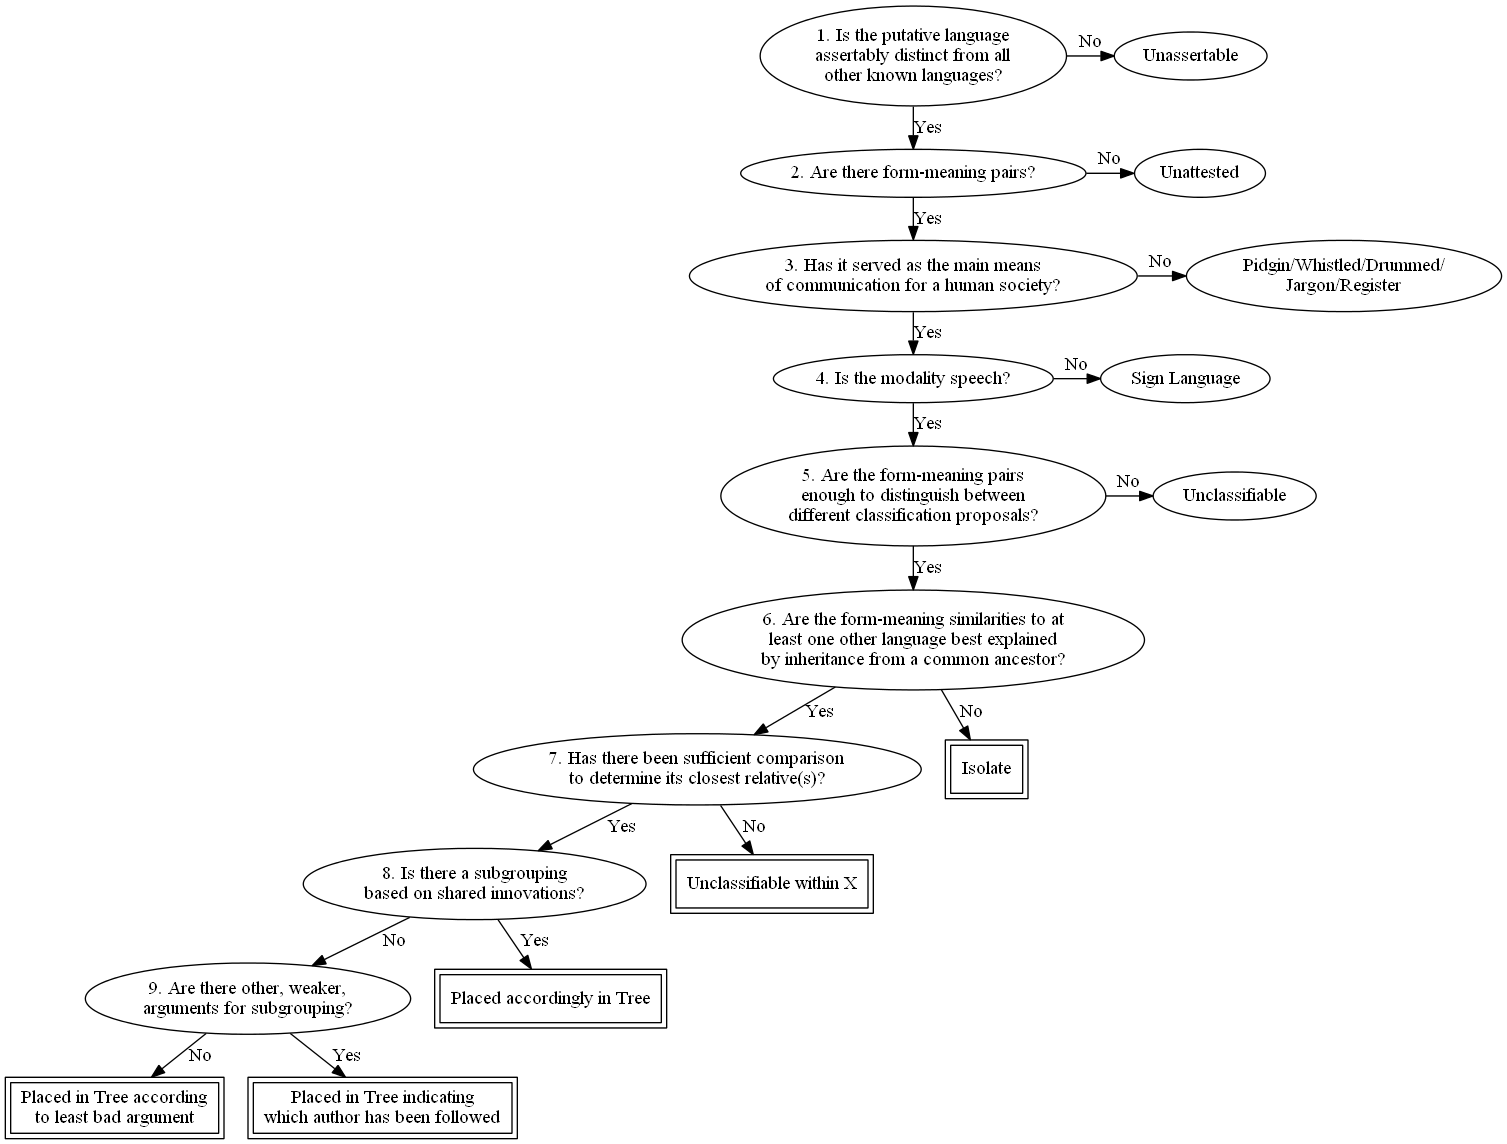
\includegraphics[width=16cm]{illustrations/Glottolog_classifying_tree.png}
\caption[Decision tree for language identification and classification in Glottolog]{{Decision tree for language identification and classification in Glottolog \citep{glottologlanguoids}.}}
\label{glottolog_class_tree}
\end{figure}

In the quote above from Glottolog on ``distinctiveness'', the editors state that one can use language data and/or reports on mutual intelligibility. When empirical data on mutual intelligibility is missing, ``an approximate minimal requirement is 50 items or so of basic vocabulary'' needed for determining the distinctness of a language and where it should be placed in a genealogical tree  (\citet{glottologlanguoids} and Hammarström p.c.). This is similar to the lexical similarity measurements used by the SIL.
%and Hammarström (p.c.) has confirmed that is what is needed for distinctiveness as well (at least). SIL also makes references to lexical similarity scores, it is plausible that Glottolog and SIL International do not differ dramatically in this respect and that while the precise material and cut-off points may vary: most of the time they will end up with similar classifications for the same language varieties\footnote{In a recent paper, \citep{wichmann_2019_dialects} shows that with his new method of devising lexical similarity cut-off points, SIL tends to have a bias towards splitting rather than joining. Glottolog classifications are not tested in the paper.}. 

One important difference between Glottolog and SIL International lies in how the evidence is documented. Glottolog provides references for every language identification and tree, making it possible for other researchers to examine the evidence on their own. SIL International does not consistently provide this information. While change requests to ISO 639-3 will often refer to reports etc and many language entries have references for at least part of the information provided, there are many instances where the information is not accessible to readers. While the Ethnologue website states that ``sources used for classifications are available on request by contacting the Editor'' \citep{ethnologue2019lgident}, personal correspondence with the editors revealed that the sources are incomplete and cannot be requested in full.

Glottolog also considers whether or not the putative language has ``served as the main means of communication for a human society'' \citep{glottologlanguoids}. This disqualifies most artificial languages, whistle registers, ritual speech registers and pidgins. SIL International does not discuss this particular criteria explicitly. However, among the artificial languages Esperanto is included in the catalogue but  Klingon, High Valyrian and Angosey are not. Unlike most other artificial languages,  Esperanto does have a few native speakers \citep{bergen2001nativization}, which is probably why it is included in Ethnologue. This suggests that SIL does consider something similar to Glottolog's ``main means of communication'' criteria even if they do not spell it out explicitly. Glottolog does catalogue constructed languages, pidgins etc, placing them in so-called ``non-genealogical trees''\footnote{The list of non-genealogical trees in Glottolog are: Sign Language, Unclassifiable, Pidgin, Unattested (data missing), Mixed Language, Artificial Language and Speech Register.}. These groups of languages are included in the catalogue and given glottocodes, but the editors note that they are not subject to the same process of language identification and classification as the rest.%\footnote{It is up to Glottolog's users to filter these out of the dataset should they want to only consider languoids that are clearly classified by Glottolog's principles.}).

The fact that Glottolog provides unique stable identifiers for dialects and families, as well as languages, makes it possible to represent data in finer detail than previously possible. It also allows individual scholars to make different decisions on what is and what is not a language from Glottolog, while maintaining comparability. For example, there are several language varieties spoken on the Austral islands of the Pacific. Glottolog has classified them as being one language (Austral [aust1304]) with four dialects (Ra'ivavae [raiv1237], Rimatara [rima1237], Rurutu [ruru1237] and Tubuai [tubu1240]). However, other linguists disagree and have argued that these should be viewed as four different languages due to wordlists indicating they were not sufficiently mutually intelligible at the time of the arrival of Europeans (Walworth \& François p.c.). In this dataset, these are counted as four separate languages because it appears to be more in line with the state of the world before the arrival of Europeans. It is easy to adjust for this in the dataset (and simple to undo) because the Glottolog dialect codes are linked to the language Austral [aust1304]. 

%In this case study, I have chosen to go with the classificatory decision that these should be viewed as 4 different languages. It was easy for me to change the coding of languages in my data to include these 4 different glottocodes as separate languages instead of ``Austral'' as one. If any researcher in the future wants to make another call they can access the data and run the analysis with another classification. Since there exists glottocodes for the dialects and these are explicitly linked to their language level parent - Austral - it is easy for make the switch.

Being able to refer to dialects and families with a stable identifier is useful and an important difference between the SIL International ISO 639-3 code standard and Glottolog's glottocodes. When working with cross-linguistic and cross-cultural databases, it is often useful to be able to refer to a language variety in a more granular detail than the ISO 639-3 set allows for. \citet{nordhoff2011glottolog} point out that there may be differences between dialects that are crucial to certain research that would be confused if it was only possible to refer in a stable manner to the language level and not also to specific dialects. For example, certain dialects of German make a distinction between /e\textipa{:}/ and /æ\textipa{:}/ whilst others don't. If references were not accurately tied to a language variety, this would be confusing as ``German'' would have different numbers of vowels in different sources. By providing stable identifiers for dialects as well as languages and providing a controlled hierarchy, it is possible for researchers to document their data accurately while still making it possible to aggregate up to the ``language-level'' when it is desirable. For example, Grambank and the Standard Cross Cultural Sample of D-PLACE both contain entries for specific languages and dialects. There are 158 one-to-one matches between the glottocodes of these two databases. In some cases though, the databases contain different dialects of the same language. If we were to lump dialects of the same language together in each of the datasets, the overlap increases to 183.

The definitions of language in ISO 639-3 (as described in Ethnologue \citep{ethnologue2019lgident}) and Glottolog both focus on mutual intelligibility. Ethnologue notes that intelligibility does have to be symmetric, but neither of the resources discuss multilingualism, or multidialectalism in any detail. It is possible that the world used to be much more multilingual than it is today \citep{evans2017did}, and there are still many places where communities are highly competent in many different language varieties. Ethnologue state that they focus on \emph{inherent} intelligibility, as opposed to \emph{acquired}, but in situations where languages are not formally taught but rather present in the community continuously it can be difficult to draw the boundary between inherent and acquired. The underestimation of multilingualism has significant consequences for studies of the evolution of language \citep{roberts2013evolutionary}. However, unless two languages are exclusively spoken in a fully multilingual setting and never outside of it, the total count of languages should remain the same. 

%It is not within the scope, or indeed even the aim, of the present study to provide a universal and unproblematic classification of languages. 
The language classification standards for Glottolog and SIL International do differ conceptually, and many of their differences may reflect their different aims (facilitating academic research by making references more accessible and integrated as compared to facilitating description and translation of the Bible into the world's languages). However, the counts for languages in the world that they produce are not that different in the end.

I will be using the classification of Glottolog, with a few adjustments, since it is more transparent and better referenced. It should be noted that using the ISO 639-3 results in the language count for the Vanuatu being 108, as opposed to 105 in Glottolog, which is not a huge difference. 

The aim of this chapter is to explore language diversification in Remote Oceania prior to the arrival of European people. Because of this, I have made a few adjustments to the Glottolog classifications of languages in the relevant region. Languages that have come into the region directly because of the arrival of Europeans have been excluded (Bislama, English, French etc). Furthermore, I have made three other changes from Glottolog in the classification of indigenous languages of the region based on other accounts of their mutual intelligibility at the relevant point in time\footnote{Tahitianization and dialect/language levelling has occurred, and therefore languages that used to be more different from each other are now more similar.}. Firstly: in Fiji, Glottolog's Eastern Fijian [fiji1243] is split into three languages: Southeast Fijian [sout2864], Northeast Fijian [nort2842] and Kadavu [kada1285] based on personal correspondence with Andrew Pawley and Paul Geraghty. Secondly, M\={a}ori [maor1246] is split into two languages: Morori [mori1267] on R\={e}kohou (Chatham Islands) and M\={a}ori [maor1246] on mainland Aotearoa (New Zealand). This classification is based on \citet{harlow1973regional} and personal advice from Andrew Pawley. Third and finally, as was previously mentioned, the languages of the Austral Islands have been divided from one to four based on advice from Mary Walworth and Alexandre François.

The splitting of Eastern Fijian [fiji1243] into three languages has as consequence that the total language count for Fiji as one island group based on overnight sailing distances is 8 instead of 5. When the island groups are defined in relation to whether they share at least one language, the great island of Viti Levu is paired with Yasawa into one group sporting 4 languages instead of 2 and Kadavu separates out as a separate island group with 1 language. For M\={a}ori [maor1246] the difference in language classification makes less difference. Aotearoa and  R\={e}kohou were always separated as different overnight distance island groups, each sporting one language (even though it is the same language under Glottolog's definition). For the island groups based on shared language they continue to be separated under the new classification, meaning in practice that we have yet another small Polynesian island group with one language. The situation is similar for the Austral islands. The new classification makes no difference for the island groups as defined by overnight distances, since all four are separated out from each other already. For the island groups based on shared language they continue to be separated out as different island groups. Overall the new classification results in more languages in Fiji, and more small Polynesian island groups with one language each.

\subsubsection{Grouping Islands and atolls and calculating isolation}
\label{sec:island_geo}

%When measuring language diversity, many methods do not deal well with islands and water. For example, all islands with only one language were excluded from the study by \citet{curriemace2009} on the relationship between language territory and ethnographic features. This is unfortunate, but understandable. The authors model of language diversification was not able to accurately enough deal with contact over water.

The aim of this chapter is to explore the number of languages across islands of Remote Oceania. We need a good way of grouping all of the islands and atolls (5,525 landmasses) that is not dependant on modern politics (nation states), but that reflects possible networks in prehistoric times. For this purpose we will combine two distinct approaches. The first is based on voyaging distances by canoe (Fig.~\ref{marck_group_map}), and the second is based on whether the islands have a language in common or not (Fig.~\ref{medium_group_map}). The assumption is that a group of islands is a meaningful unit for comparison if it forms a \textit{network of contact} (i.e. it is possible to maintain contact through voyaging or otherwise sustain linguistic homogeneity). 

%\citet{hauofa_1993}

\begin{figure}[H]
\centering
    \begin{subfigure}{\textwidth}
    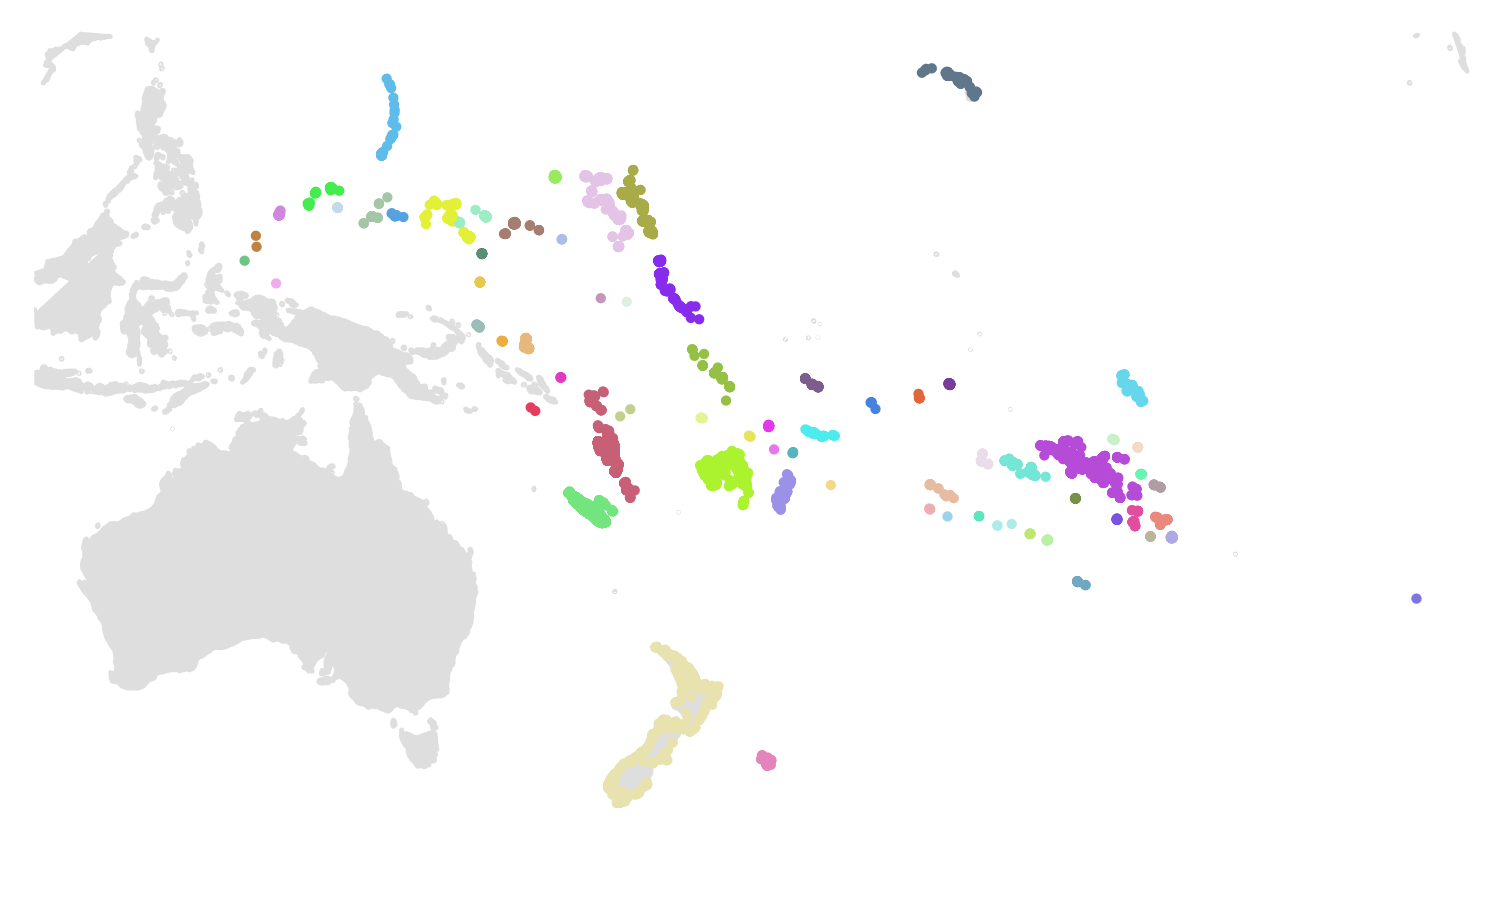
\includegraphics[width=\textwidth]{illustrations/plots_from_R/polygon_marck_group_map.png}
     \caption{Island and atolls grouped by overnight sailing distance (see main text for definition).}
\label{marck_group_map}
    \end{subfigure}

    \begin{subfigure}{\textwidth}
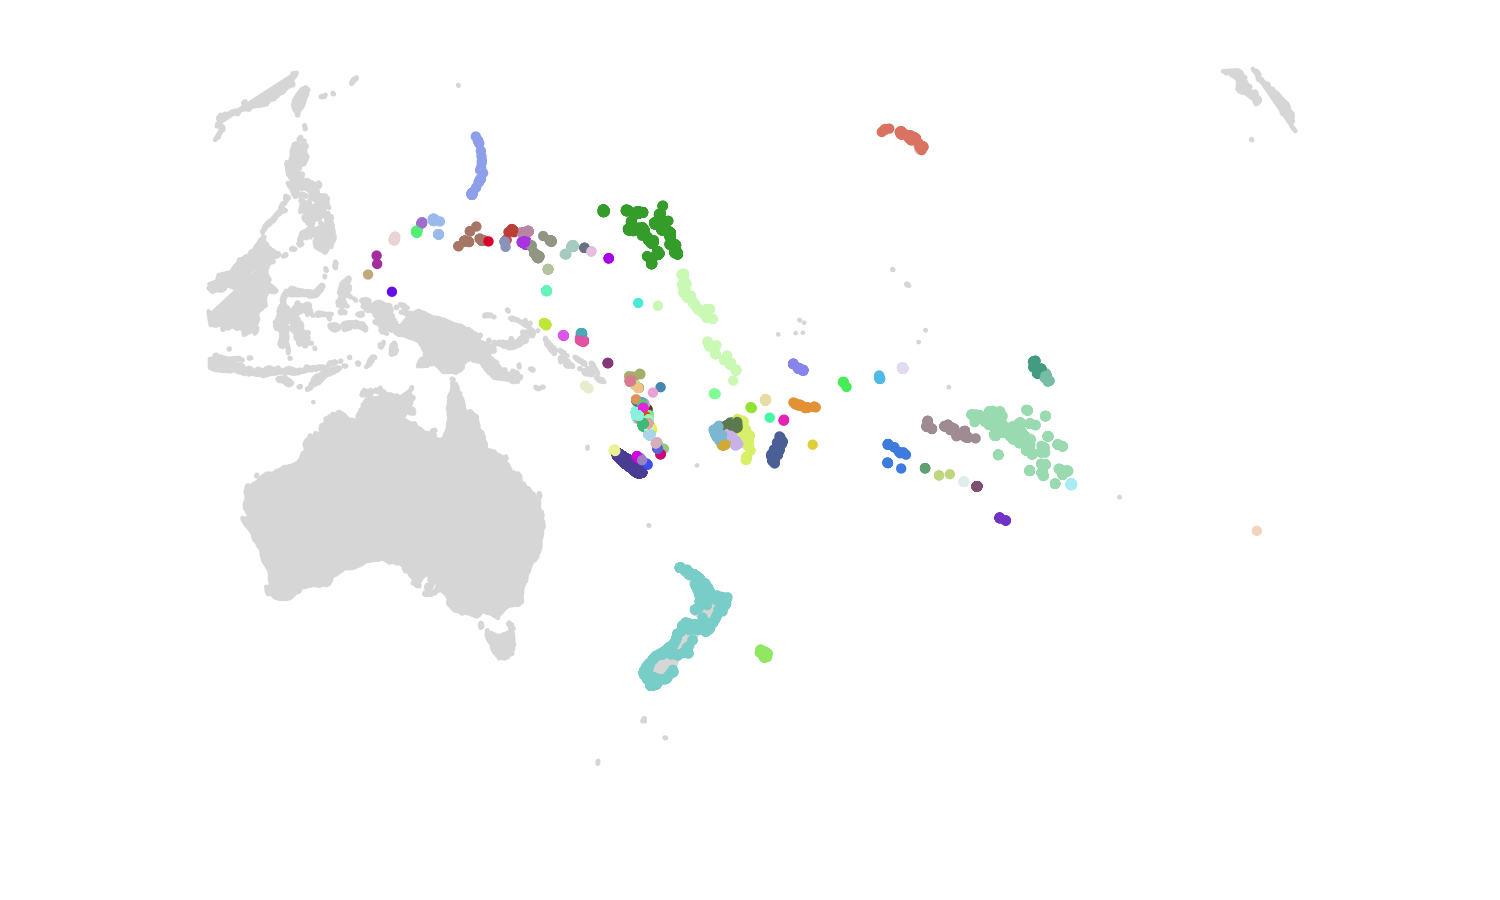
\includegraphics[width=\textwidth]{illustrations/plots_from_R/polygon_medium_group_map.png}
\caption{Island and atolls grouped by shared language(s).}
\label{medium_group_map}
    \end{subfigure}
\caption{{Island groupings for chapter \ref{chapter_pol_complex}. Colour indicates group.}}
    \label{fig:island_groups}
    \end{figure}
    
\citet{mark_1986, marck2000} uses 100 miles as an approximate limit of an overnight voyage in a traditional canoe, and infers that this most likely represents a reasonable distance which might be travelled regularly to stay in contact within a community. If two islands are within 100 miles of each other, they are classified within the same overnight-distance group and covered by the same colour in Fig.~\ref{marck_group_map}. An example of this is that the southernmost island of the Solomons, the Santa Cruz islands of the Temotu province, is within overnight voyage distance of the northernmost islands of Vanuatu. This is why the islands of Vanuatu and Temotu are the same colour in Fig.~\ref{marck_group_map}. However, the two island chains of the Marshall Islands, Ratak and R\={a}lik are separated when islands are grouped by this principle despite sharing a common language and being one modern country. This is also the case for the eastern islands of the Tuamotu, with the Reao atoll being classified as a separate island group from the main islands of the Tuamotu archipelago. We will refer to these island groups as \textit{overnight distance groups}. 

If two islands share a language, they are classified as of the same island group in Fig.~\ref{medium_group_map}. For example, all islands of the Tuamotu archipelago (where Tuamotuan [tuam1242] is spoken) are coloured the same, even though they are grouped into several separate island groups by the overnight distance approach. Vanuatu, being a land of great language diversity, has a different colour for almost every island. Another example is the Tungaru islands (western islands of Kiribati) and Tuvalu which actually share a language. Most people of the country of Tuvalu speak Tuvaluan, but there is one island, Nui, where Tungaru (Gilbertese [gilb1244]) is also spoken \citep{faaniu1983tuvalu, macdonald_2020, omniglot_tuvaluan}. Therefore, they are coloured the same in Fig.~\ref{medium_group_map}. We will call these island groups \textit{shared language groups}.

These two principles, overnight sailing distances and sharing a language, have been applied consistently over all islands and all languages using data available in the Ethnologue \citep{ethnologue22}, Glottolog \citep{glottolog40} and in some cases specialist literature (\citet{faaniu1983tuvalu,charpentier2012linguistic, francoisetatl2015, macdonald_2020, omniglot_tuvaluan} and a map of indigenous languages of New Caledonia published by CNRS-LACITO), with only two exceptions. The Micronesian atoll Mapia and the Polynesian outlier atoll Nukuria are technically within an overnight sailing distance of the coast of New Guinea. However, since that would mean averaging over data from outside of Remote Oceania and since they are \emph{almost} far enough away, they have been classified as separate island groups. In the end, there was too little data available for these two atolls for them to be included in the models. They appear in Fig.~\ref{fig:island_groups} with separate colours.

%\footnote{This map has been produced by the team of Oceanic linguists at CNRS-LACITO, but it has never been officially published. It appears in other academic papers, for example \citet{speedy2013reflections}, but regretfully it is not possible to provide a stable bibliographical reference to it independently.}.
For each of these island groups, absolute latitude, total area and shoreline were calculated from the Global Self-consistent, Hierarchical, High-resolution Geography Database (GSHHG), version 2.3.7 \citep{wessel1996global}. The analysis of this chapter also includes the ratio of shoreline to area, as we may expect islands groups with many small islands and atolls to be different from those with one large island, even if their overall area is the same\footnote{Thank you to the anonymous examiner who suggested including this.}. Area and shoreline were both log-transformed (log 10). This was done both to be in line with previous studies \citep{gavin2012island} and because the distributions had extreme outliers (New Caledonia and Aotearoa/New Zealand). Such outliers end up driving the model in a manner that is not representative of the overall sample. By logging these variables the overall structure and order of data-points remains the same but the influence of the extreme outliers is reduced.

%ANU CartoGIS also provided data for the water area which is covered by the overnight sailing distances, the light-blue shaded areas of Fig.~\ref{RO_overnight_coloured_dots}.The area between and around islands is important because it provides access to fish and seafood (c.f. rice or wheat fields to agriculturalists or tundra and taiga to reindeer herders), islands which have less territory of this kind but equal land area to another island may be able to support fewer people. For the island groups defined by shared language which are smaller than Marck groups, the water area was assigned proportionally to the islands landmass size in comparison to the entire Marck group's landmass (i.e. Malakula makes up)

A score of isolation was also calculated based on the GSHHG-data as well. There are many different ways of measuring island isolation. \citet{rolett2004environmental} use two measures, distance from home island to island which is >25\% larger than home island and distance to island >75\% larger than home island. \citet{gavin2012island} use distance to the Asian continent (after considering three other measurements). The ``Isolation index'' of the Islands database \citep{dahl1991island}  is calculated as follows: (distance to nearest equivalent or larger island)$^{0.5}$ + (distance to nearest island group or archipelago)$^{0.5}$ + (distance to nearest continent)$^{0.5}$. \citet{weigelt_2013} present an overview and comparison of 17 different island isolation measurements used in biology and conclude that it is advisable to consider stepping-stone pathways, larger islands (besides continents), climatic similarity and the area of surrounding landmasses when studying the richness of species in relation to island isolation.

In light of this, and given the data available, a simple isolation metric has been calculated. This measurement consists of \textit{the distance from the largest landmass of each island group to the closest landmass which is the largest in its island group}. This is essentially a distance of ``home island'' to closest other ``home island''. For example, for Hawai'i the largest island is the Big Island. The closest island to the Big Island which is also itself the largest in its group is part of the M\={a}ngarongaro atoll (also known as Penrhyn or Tongareva). This distance is 3,191 km. This is the largest distance for our isolation measurements, therefore Hawai'i is the most isolated island group. The metric is calculated separately for the overnight distance groups and shared language groups and was also logged (log 10) for the same reasons that area and shoreline was logged.

Each island group is associated with all the languages spoken there, based on information in the various sources cited earlier for defining groups by shared language. Naturally, some islands will have many languages assigned to them, most notably Santo and Malakula in Vanuatu with 24 and 33 languages respectively. Other languages are spread out over many islands and atolls. Tuamotuan [tuam1242] is for example assigned to 1,302 distinct landmasses (in this dataset atolls and reefs that are above water appear as several small landmasses). For shared language groups, these landmasses are all joined under the label `Paumotu'. However, as defined by overnight sailing distances this archipelago is 10 separate island groups: Paumotu, Hereheretue, Tureia, Morane, Marutea, Nukutavake, Puka-Puka\footnote{Not to be confused for Pukapuka. Puka-Puka is a place-name for an atoll in French Polynesia and Pukapuka is an atoll in the Cook Islands.}, Napuka, Tatakoto and Reao. Each of these 10 island groups have a language count of one. The fact that it is the same language is not accounted for (\citet{gavin2012island} also arrange their data like this).

These two island groupings form the unit of analysis for our statistical models. They are associated with number of languages, rainfall, oldest time of settlement, isolation, temperature, etc. The statistical model is trying to predict the number of languages (our response variable) based on these factors. For both island groupings, the distribution of languages is highly positively skewed. Fig.~\ref{dist_lg_medium} shows the distribution for shared language island groups. Most island groups have just one language and a few have very high numbers. This pattern is even more pronounced in the groups based on overnight distances (because all of the islands of Vanuatu and Temotu province are one island group). Statistically, the distribution of languages over both sets of island groups are over-dispersed (the variance is higher than the mean).
This requires that we use a different kind of model than if the distribution had been less skewed (see section \ref{pol_complex_method}). This issue was also faced by \citet{gavin2012island} in their study of environmental factors in language diversification in the Pacific. They chose another approach, a reciprocal transformation, based on model fitness compared to two other kinds of transformations of the response variable.

\begin{figure}[H]
\centering
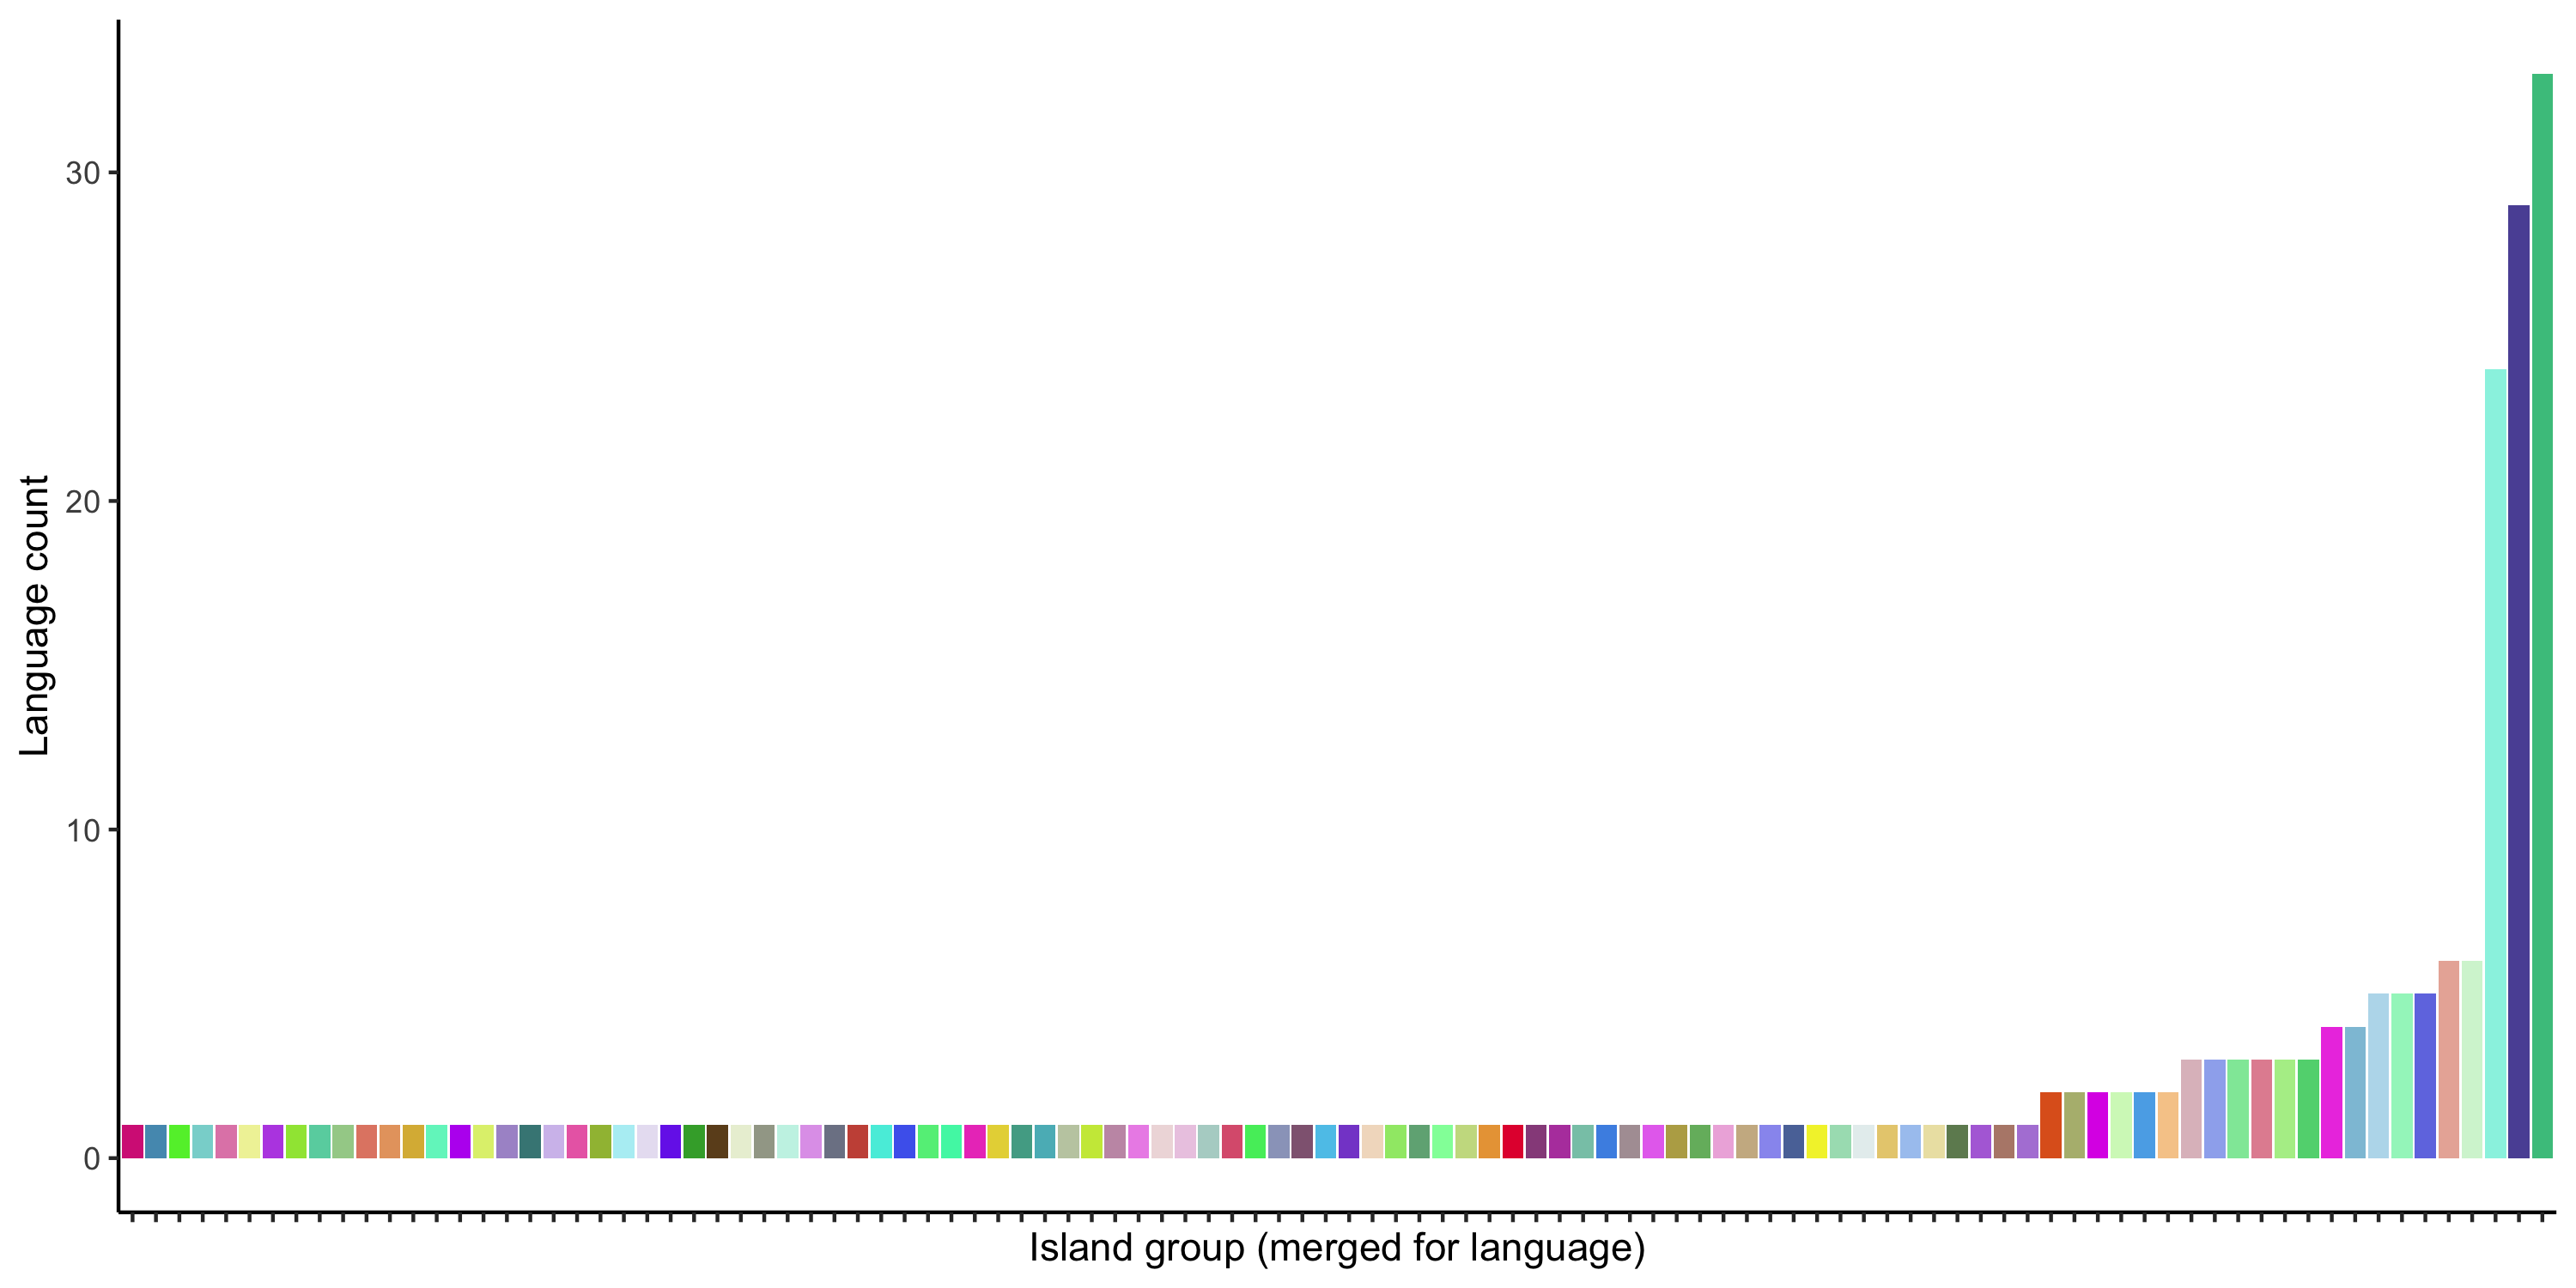
\includegraphics[width=13cm]{illustrations/plots_from_R/Lg_distrubition_medium_island_group_lg_merged.png}
\caption{{Distribution of languages per shared language island group.}}
\label{dist_lg_medium}
\end{figure}

\subsubsection{``Political complexity''}
\label{prediting:sec:pol:complex}
The hypothesis tested in this chapter relies on a systematic measure of political structure across societies. The most widely used variable in this regard is variable 33 of the Ethnographic Atlas \citep{EA_1971}: ``jurisdictional hierarchy beyond local community'' (EA033). This section gives an overview of how this variable is defined and its distribution in Remote Oceania. 

The Ethnographic Atlas was first published in 1962 and is one of the datasets included in D-PLACE \citep{d_place_all}. EA033 is widely used to represent ``political complexity'' in studies of cultural evolution. This variable has been used to study the relationships between the area a language covers, subsistence strategies and political organisation \citep{curriemace2009}; processes of rise and fall of ``political complexity'' in South-east Asia and the Pacific \citep{currie2010rise}; the spread of Christianity in the Pacific \citep{watts_2018}; and coevolution of intensive use of natural resources and political structure \citep{sheehan2018coevolution}.  

In all of the studies referenced above, EA033 is used as a way of quantifying vertical political structure within a society beyond the local community. In the rest of this chapter we will be referring to this variable as ``political complexity''. There is a separate variable (EA032) for jurisdictional hierarchy \emph{within} local communities. ``Local community'' is in the ethnographic/anthropological literature is defined as the ``maximal group of persons who normally reside together in face-to-face association'' \citep{yale1945outline}. The size and distribution of local community may vary greatly. For Remote Oceania, the Ethnographic Atlas records entries ranging from less than 50 (Ponape) to between 400-1000 (Tikopia).

``Society'' is not defined explicitly in most of the literature, but it is sometimes used interchangeably with ``ethnic group'' or ``culture''. \citet{roger1981cultural} write:

\begin{quotation}
\noindent\emph{[A]ll the communities that are connected politically and economically (and hence comprise a kind of total social system) can be taken as comprising a \textbf{society}. Characteristically, a society comprises a total social system whose members share a common language and cultural tradition}. 
\begin{flushright}
\citep[22]{roger1981cultural} 
\end{flushright}
 \end{quotation}

%\footnote{Ironically, later in this section \citet[23]{roger1981cultural} quote \citet[422]{schwartz1978culture} in saying that the ``Manus people'' as a society are easily linguistically bounded, when linguists have counted up to 19 languages on the island \citep{glottolog40}. In D-PLACE \citep{d_place_all} the society ``Manus'' in the Ethnographic Atlas is specifically linked to one language out of these 19, Titan [tita1241].} 

It is not possible to give more detail to the definition of ``society'' as employed in the Ethnographic Atlas dataset, but it does seem to correspond to ``language community'' to a great extent. In cases where societies are multilingual (c.f. \citet{evans2017did}), it is less likely that the definition relies on one shared language. It is, however, unclear how such cases are represented in the Ethnographic Dataset.

In some instances, it may be that ``local community'' and ``society'' are one and the same. For example, the total population for the ``ethnic group'' (variable EA202) of the society Tikopia is 1,300 which is not that much larger than the mean size of the local community (EA031) noted above. On the other hand, the total population of the ethnic group of Ponape is 8,000, which would result in an estimate of 160 local communities given the value of mean size of local community (EA031).
  
Political complexity (EA033) as a variable is observed per society, i.e. it does \emph{not} capture relationships \emph{between} distinct societies. It also does not track the political structure \emph{within} the local community\footnote{Ethnographic Atlas variable 32 captures jurisdictional hierarchies \emph{within} local communities.} or \emph{horizontal} political relationships within a society (e.g. political relationships between equal genealogical groups). It specifically measures \emph{vertical} jurisdictional levels \emph{within} a given society, \emph{beyond} the local community. Furthermore, it targets ``jurisdictional'' authority --- not just the existence of rank. In other words, the levels of authority need to be tied to some kind of jurisdictional power, most likely the power to exert punishment for transgressions and possibly also to declare warfare upon other societies. This is important because readers unfamiliar with these particular characteristics of ``political complexity'' as defined by EA033 may assume that horizontal relationships or relationships of debt (i.e. not jurisdictional) are included. 

The possible values societies can take for this variable of political complexity are:

\begin{enumerate}
\item No levels (no political authority beyond community)
\item One level (e.g., petty chiefdoms)
\item Two levels (e.g., larger chiefdoms)
\item Three levels (e.g., states) 
\item Four levels (e.g., large states)
\end{enumerate}

\citet{giuliano2018ancestral} write: 

\begin{quotation}
\noindent\emph{[I]f the local village chief is the highest level of authority, and he or she does not answer to anyone above them, then the variable would take on a value of [1]. If above the chief, there was a district leader, then above this, there was a territory leader, and above this a provincial leader, and above this the paramount chief, then this variable would take on the value of [5].} 
\begin{flushright}
\citet[9]{giuliano2018ancestral}
\end{flushright}
\end{quotation}

This way of characterising political structure aligns well with ethnographic accounts of political structures in Western Polynesia, as we have for example seen in descriptions by \citet{sahlins63}. Consider Fig.~\ref{meleiseapyramid} \citep[22]{meleisea1995} for example, which illustrates the ideal characterisation of political power in S\={a}moa. The village level (\emph{matai} titles) corresponds to value 1 for EA033, subdistrict (\emph{ali'i} titles) level 2, district level (\emph{ali'i pa'ia / ao} titles) 3 and nation (\emph{tafa'if\={a} / tupu} titles) corresponds to level 4. S\={a}moa is however coded as level 3 since paramount titles are very unstable in the archipelago, even though they theoretically do exist.

%\footnote{There exists some variation in the literature as to where to start this scale, either with 1 = no political authority beyond community, or 1 = missing data. We will be using the default scale in the Ethnographic Atlas Codebook from \citet{gray1998ethnographic} here and adjust quotes from other publications to this scale so as to reduce confusion.}

\begin{figure}[H]
\centering
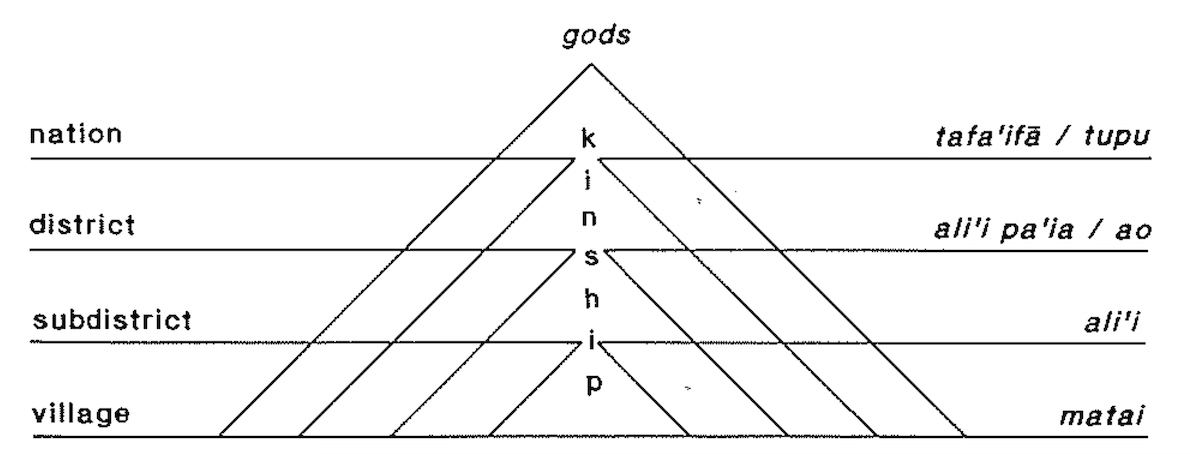
\includegraphics[width=13cm]{illustrations/pyramid_meleisea.png}
\caption[Illustration of traditional political organisation of S\={a}moa.]{{Illustration of the traditional political organisation of S\={a}moa from \citet[22]{meleisea1995}.}}
\label{meleiseapyramid}
\end{figure}

However, this framework is less easy to apply to the Melanesian islands of Remote Oceania where political structure often is described more in terms of autonomous and equal groups organised into horizontal structures such as exchange networks --- both within and between societies (c.f. \citet{bonnemaison1996graded} and \citet{huffman1996trading}). \citet{bolton1998chief} points out that the very concept of ``chief'' is new to Vanuatu, writing that chiefs were first introduced by Europeans to fill the role of ``representative for a community towards outsiders'' and then transformed into ``representative for traditional culture (kastom)'' \citep[185]{bolton1998chief}. In this thesis, political complexity is assumed to be a proxy measurement of social network cohesiveness (c.f. \citet{grace_1992_aberrant}). Differences between modern Vanuatu ``chiefs'' and pre-European political structures are therefore unlikely to be large enough to give rise to dramatically different scores in this metric. As has been shown in previous studies, while this metric may be coarse grained and not capture all the nuances of political life in the region, it appears to still be useful in testing hypotheses such as the one investigated in this chapter.

%, it may still be valuable to us in a) operationalising the hypothesis of Turner/Sahlins/Pawley

%Given this, what does it mean to go looking for ``chiefs'' and ranks in Vanuatu and what would descriptions of such institutions in ethnographies actually capture?

%Problematic as this variable may be in faithfully capturing relevant facts of political structure in all the societies in our sample, it may still be valuable to us in a) operationalising the hypothesis of Turner/Sahlins/Pawley and b) capturing something about social networks and group identity (even if it only measures this by proxy). In this case study, we are testing the hypothesis that societies that are rules by ``powerful chiefs'' and have more levels of vertical jurisdictional structures are slower at diversifying than societies with a more egalitarian/horizontal structure. Given that this is what we are testing, I believe that variable EA033 can still serve us well even if it does not capture the nuances of power structures equally well throughout the region.

Given our language classification earlier, there are 233 language communities in our maximal sample. The ethnographic data is collected per society, and as was mentioned earlier it is possible for different societies to have the same language. Societies with the same language have been merged and our smallest cultural units of analysis are the language-society\footnote{American S\={a}moans and Upolu S\={a}moans were the only societies that needed merging in this fashion.}. Each language is associated with the islands and atolls where it is described as spoken. The full geographical dataset contains 5,525 unique landmass polygons\footnote{The total number of polygons in the geographical dataset is 9,750, but this includes New Guinea and uninhabited islands (Phoenix Islands for example). 5,525 is the number of unique polygons that can be associated with a community of Remote Oceania.} which have been grouped into our smallest geographical unit of analysis: 104 shared language island groups. In the analysis, we will also be aggregating the islands into 69 overnight distance groups.

D-PLACE has a value recorded for political complexity for 44 ``language-societies'' in Remote Oceania. There have also been more recent studies where other authors have added more entries. We will be using additional data-points from a separate publication by \citet{sheehan2018coevolution}, resulting in another 27 data-points. There was an overlap between these two datasets, 26 language-socities having a coding both in the original Ethnographic Atlas dataset in D-PLACE and in Sheehan et al. Of these, 11 societies (i.e. 43\%) were coded exactly the same. Upon closer investigation of the instances where the coding differed, I found that Sheehan et al often had access to \textit{more} data, more \textit{comprehensive} data and more \textit{recent} data. Each of these instances was re-evaluated, and most often the coding from Sheehan et al was kept\footnote{I am grateful to Sheehan for very helpful personal correspondence during this process.}. The data was also further supplemented with information from \citet[201]{bonnemaison1996graded}, resulting in 66 more data-points in Vanuatu. 



%For the instances where they had represented the same society with different values, I consulted the relevant ethnographies myself and made my own coding decision. In the most cases, my evaluation of the data sided with the interpretation by Sheehan et al. Given that Sheehan et al have access to more recent and more comprehensive ethnographic material, it shouldn't be surprising that they have made different decisions and that a second look is more likely to agree with their evaluation than the older dataset. 

%Reading ethnographies is difficult, and involves a lot of interpretation and additional knowledge of context. It is not that dissimilar from reading grammars (which I have more experience with). If anything, reading ethnographies is tricker than reading grammars since there is more variation in how to describe ``a culture'' than there is on how to describe ``a language''. I had the fortune to be able to correspond with Sheehan and discuss particular cases in greater detail, which was very valuable. During these investigations, I also came across a typology of political systems in Vanuatu compiled by \citet{bonnemaison1996graded} (see Fig.~\ref{Bonnemaison_map}) which provided more data-points. In reading \citet{bonnemaison1996graded, sahlins63},  and discussing with Sheehan, I concluded that it is possible to infer a level of 1 for EA033 where Bonnemaison describes a society as having a ``grade-taking system''. It is however unclear if a coding of 2 or higher can be made when societies are described as ``chieftainship of ``Polynesian'' type, so I did not record those observations in our dataset. In the end, I arrived at a dataset that had good enough coverage for this study (130 out of 233 language-societies and 61/105 island groups) and that I felt confident represented the description of these societies well. 

%\begin{figure}[H]
%\centering
%\includegraphics[width=13cm]{illustrations/Bonnemaison_1996_vanuatu_map.png}
%\caption{{Map of traditional systems of power in Vanuatu, from \citet[201]{bonnemaison1996graded}.}}
%\label{Bonnemaison_map}
%\end{figure}


It should be noted that this data does not represent the state of these societies for the entire period between first settlement and European arrival. As \citet{meleisea1995} writes, anthropology of the Pacific often depicts an unrealistic ``ethnographic present''. For example, \citet[185]{schoeffel87} writes about the shift in the political world of S\={a}moa under the rule of Salam\={a}sina which gave rise to a greater distinction between two kinds of chiefs: \emph{tul\={a}fale} and \emph{ali'i}. \citet[249]{kirch2017road} also mentions this distinction, but notes that it mainly came to prominence in the 1500's. As a way of avoiding this problem, the D-PLACE database \citep{d_place_all} contains information on the focal years of the description. The data for the variable on political complexity in Remote Oceania varies from 1800 (Hawai'i) and 1940 (Vanua Levu). This chapter assumes that even more recent data may sufficiently accurately reflect the state of past societies, such that it remains useful for testing the central hypothesis.

Fig.~\ref{pol_complex_map} represents the coding of political complexity for the relevant societies. A more detailed table can be found in appendix \ref{Pol_complex_table}. While it is indeed the case that societies of Melanesian Remote Oceania tend to have lower levels of political complexity, it should be noted that many societies in Polynesia and Micronesia also score a value of 1.

\begin{sidewaysfigure}
\centering
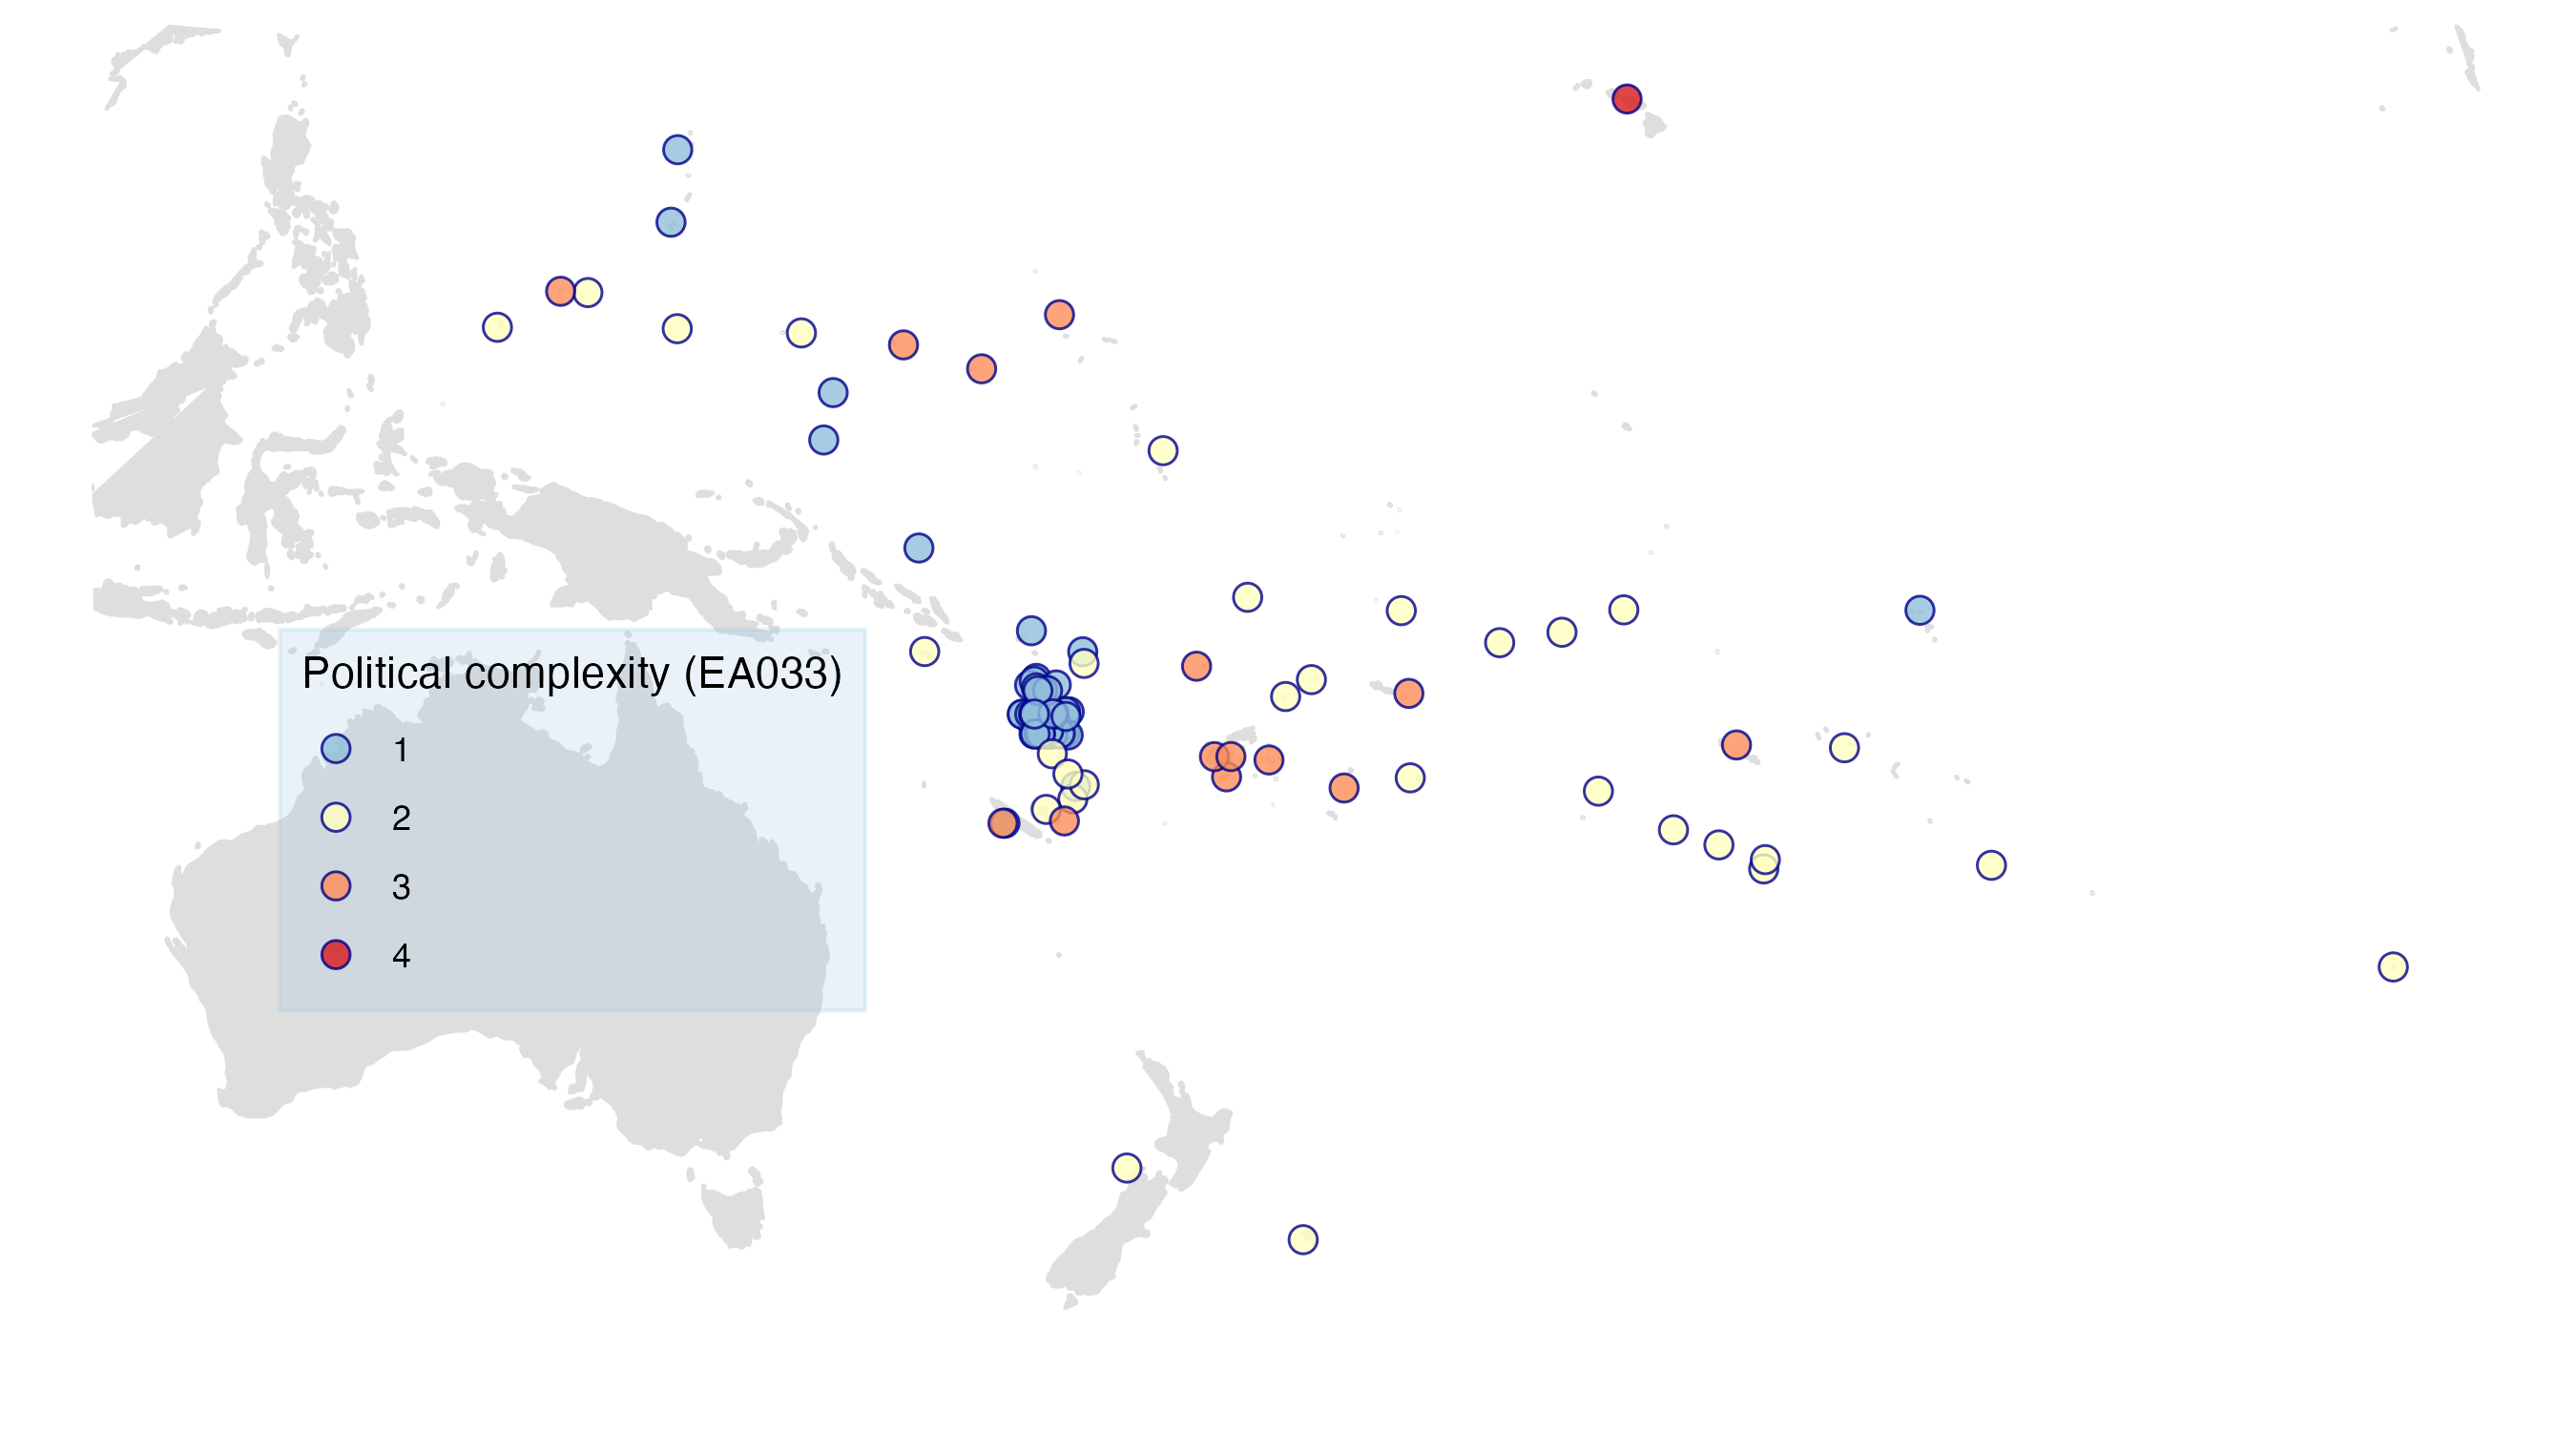
\includegraphics[width=19cm]{illustrations/plots_from_R/map_pol_complex.png}
\caption[Map of Remote Oceania: Political complexity]{{Map of Remote Oceania with associated values for political complexity (EA033).}}
\label{pol_complex_map}
\end{sidewaysfigure}

For the calculations of this chapter, the average political complexity per island group was used. This may differ for island groups clustered by overnight distances or based on sharing a language.


\subsubsection{Waves of settlement}
\label{pol_complex_sec_dates}
In order to test whether political complexity is driving language diversification in Remote Oceania, we need to control for other relevant variables --- in particular time depth of human settlement. The time of settlement indicates how long a community is likely to have been in a certain place. It can also be a proxy measurement of how similar neighbours are likely to be. If a place has only been inhabited by humans for a short amount of time, then it is likely that the communities that exist there today are not so different from each other. However, in order to take into account similarity between communities fully it is necessary to explicitly include measurements of cultural similarity or phylogenetic distance --- which is not part of the methodology of this chapter, but is left for future studies.

For most islands in our dataset, there is at least one archaeological study indicating time of first settlement. The archaeological data here is mainly based on an overview of the literature by \citet{rieth_cochrane_2018}, supplemented by the following studies: \citet{intoh2007reconnaissance, intoh2008ongoing, carson2012recent, kirch2012basline, Napolitano_et_al_yap, ellis2012saipan} and \citet{levin_seikel_miles_2019}. 

For most of the island groups, the labels provided in \citet{rieth_cochrane_2018} or the other sources neatly corresponded to the island groups in our data (e.g. Mangareva = Mangareva). However, sometimes the label refers to a larger area, this is the case of ``Austral Islands'' which in our dataset is broken down into Rimatara, Tupuai, Ra'ivavae and Rurutu respectively. In such cases it is assumed that the time can be generalised over the smaller island groups (this is also the case for the political complexity metric). Furthermore, some island groups have not been subject to archaeological research, but they are known to have been settled in association with another place which has been studied. For example, while there have been no archaeological excavations on the Sorol atoll of Micronesia, it is known to be closely related to Ulithi \citep[23]{quackenbush1968sonsorol} and it is likely that it was settled at a similar time. In such cases, the time depth is inferred based on information from nearby islands. For every island, the table in the appendix \ref{dates_table_appendic} lists the label of the island group in the source and if the settlement timing has been inferred based on evidence from nearby islands or not.

Archaeological dates are based on radiocarbon findings which are calibrated based on conditions at the excavation site and other finds there. There exists different calibration methods\footnote{Radiocarbon calibration is the process by which radiocarbon years are converted into calendar years. Because the ratio of atmospheric $^{14}$C/$^{12}$C, which is a key element in this process, has not been stable historically, different methods exist and these may produce different results.}. In order to make the dates from different sites directly comparable they need to be re-calibrated in the same way. It was not possible to access all the necessary information on each publication and re-calibrate the dates appropriately. Instead of using the raw dates from the different studies, the islands have been sorted into a settlement order with twelve waves based on the dates in the literature and descriptions of what was settled in the same wave. Fig.~\ref{dates_map} illustrates the settlement wave order per island. Exact dates and references are found in appendix \ref{dates_table_appendic}.

For comparison across island groups, the oldest settlement order per group was used. Unfortunately, this means that settlement data for Polynesian outliers in Southern Vanuatu, who arrived much more recently, is ignored.

\begin{sidewaysfigure}
\centering
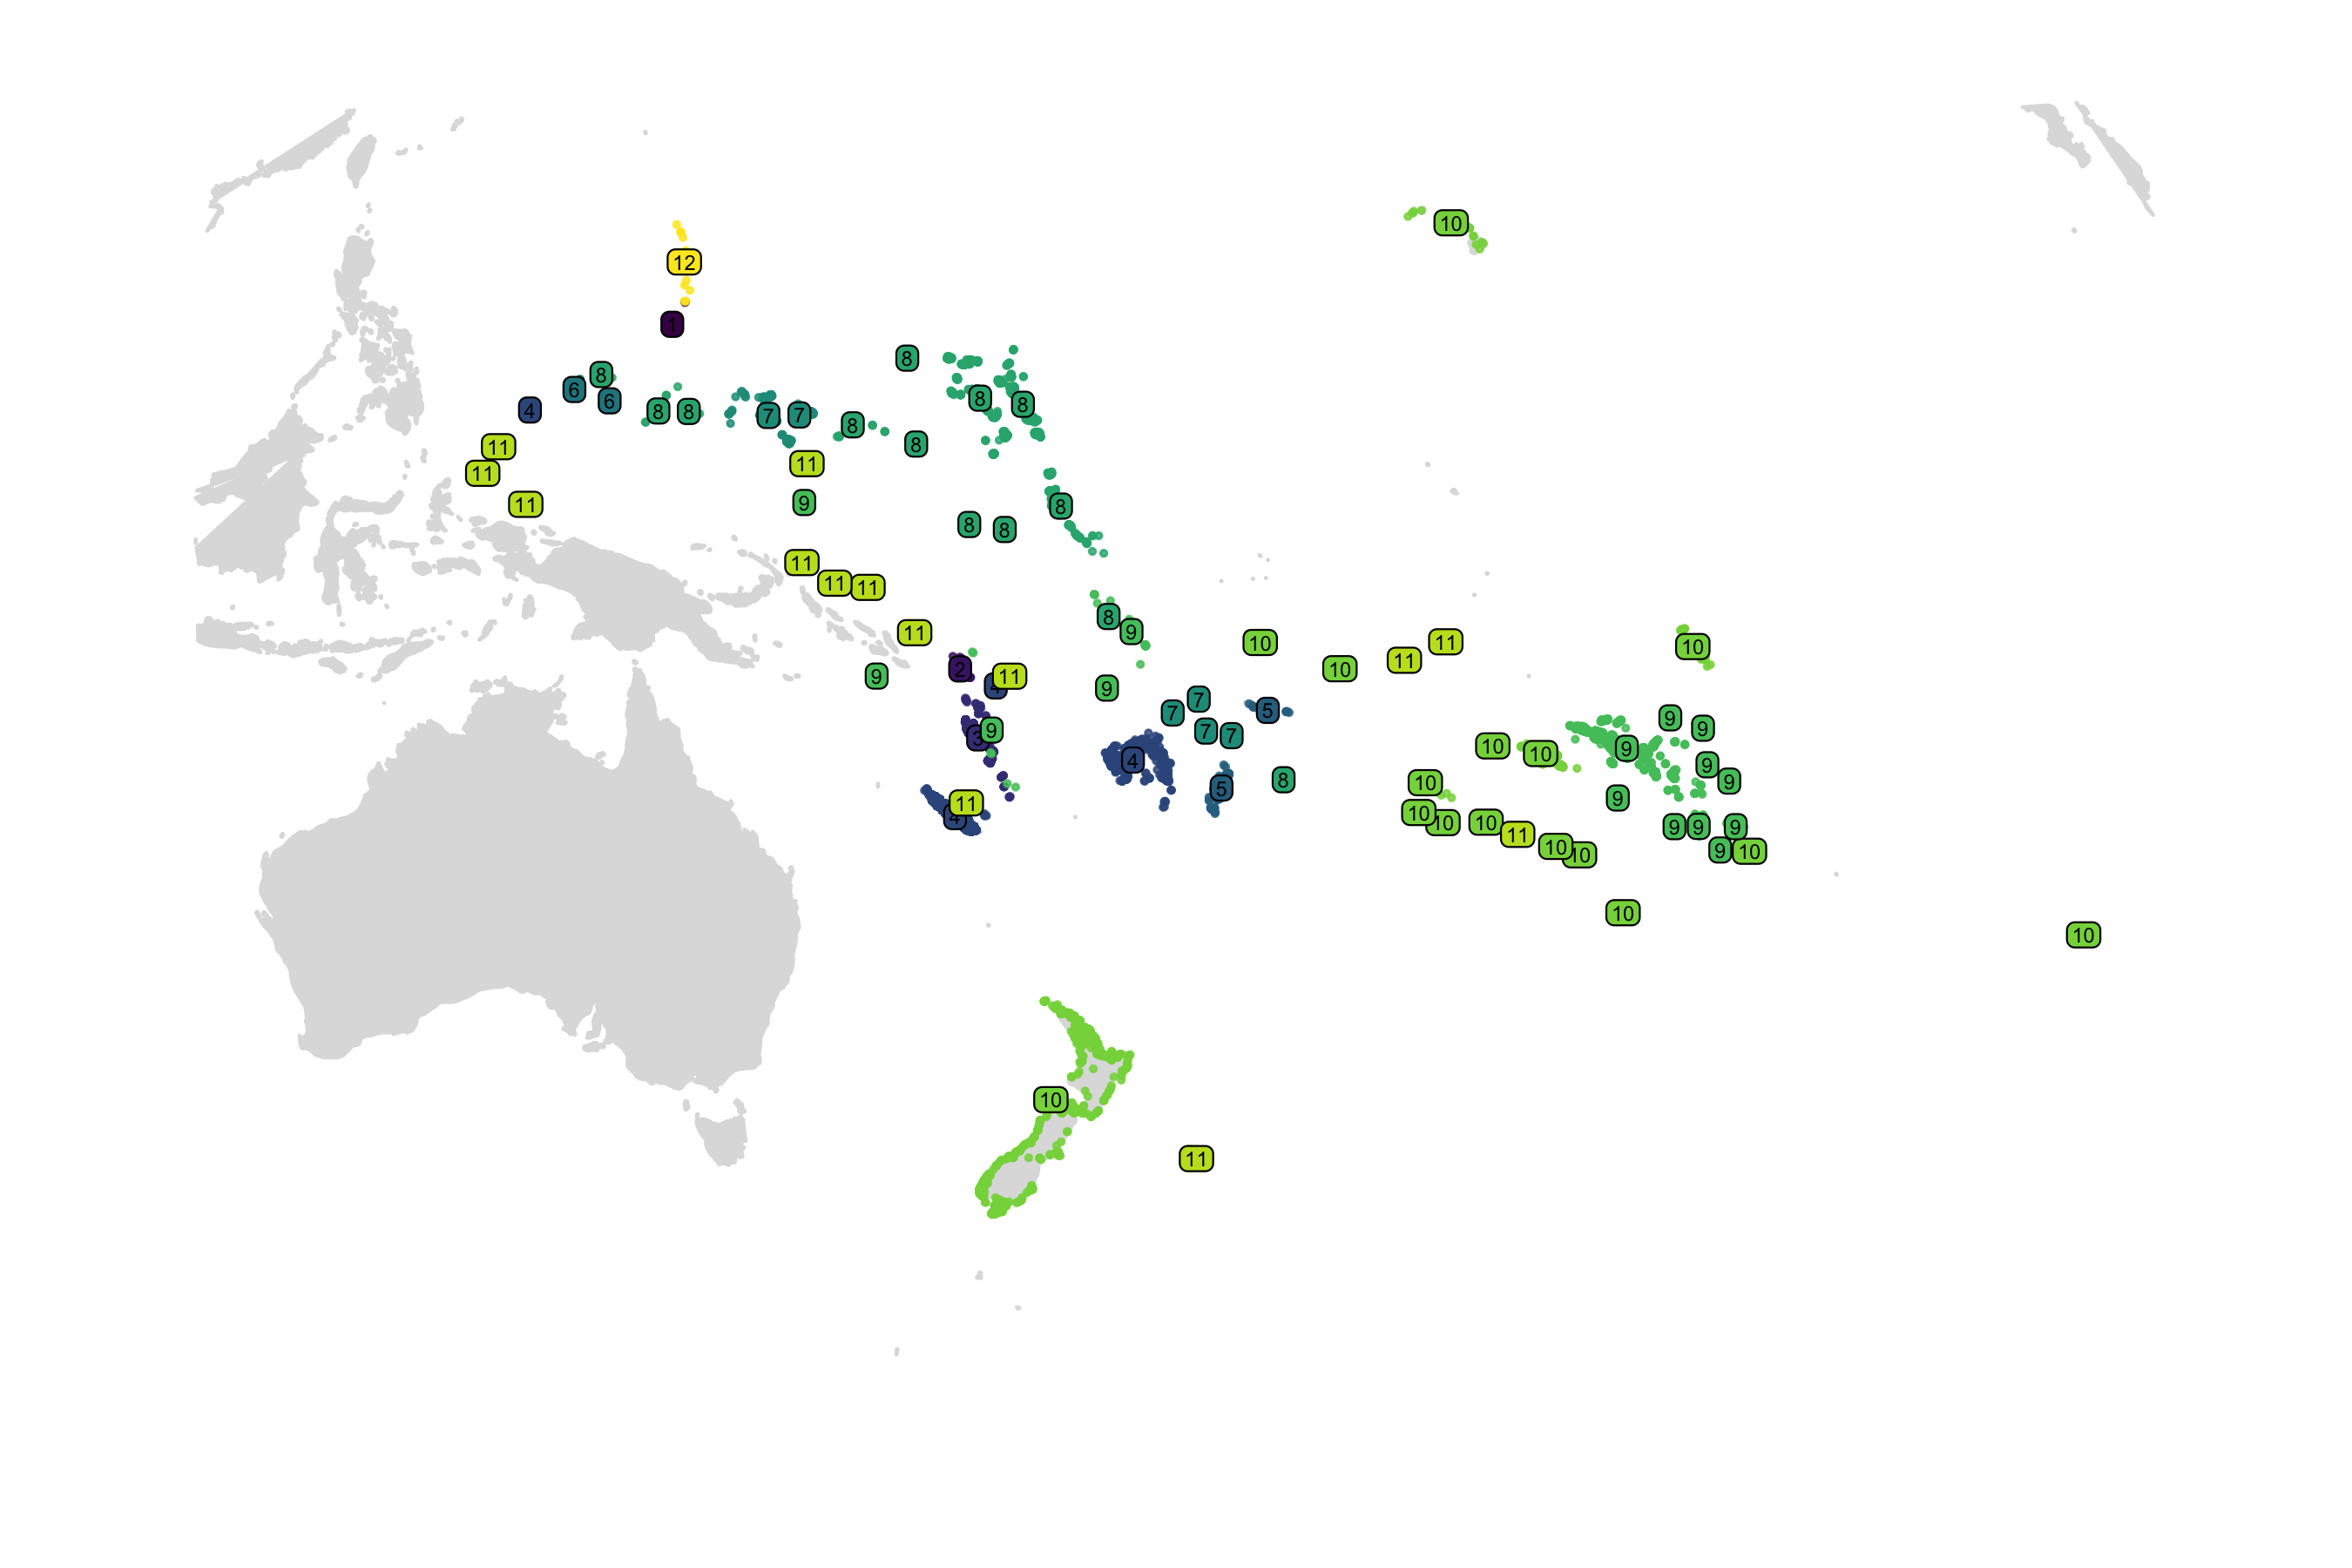
\includegraphics[width=19cm]{illustrations/plots_from_R/Map_RO_dates.png}
\caption{{Map of island groups in Remote Oceania labelled with settlement order.}}
\label{dates_map}
\end{sidewaysfigure}

\subsubsection{Other environmental factors} 
As previous studies of language diversification have shown, environmental factors such as latitude\footnote{Latitude is included to make the methodology comparable to other studies in this field. It should be noted that it is taken to be a proxy-measure of other environmental variables such as Net Primary Production which was not possible to include (c.f. \citet{hillebrand2004generality}). However, it is likely that the rainfall and temperature variables are capturing the most relevant aspects of this. Thank you to the anonymous examiner who pointed this out.}, area, temperature and rainfall can predict the number of languages in a given area to a significant degree \citep{ greenhill2015demographic, gavin2017process, Pacheco_Coelho_2019, hua2019ecological}. For this study, environmental variables were chosen based on previous research and data availability. 

We will be using measurements of (absolute) latitude, area, shoreline, ratio of shoreline to area and isolation based on the landmass polygons from the Global Self-consistent, Hierarchical, High-resolution Geography Database (GSHHG) version 2.3.7 \citep{wessel1996global} (see section \ref{sec:island_geo}). For temperature and rainfall statistics, the variables were extracted from the ecoClimate database \citep{ecoclimate} for the relevant locations. We are including measurements for the annual mean temperature and rainfall and for their respective seasonality (variation over the year).

The following variables from the ecoClimate database are used:

\begin{itemize}
\item Bio1: Annual mean temperature
\item Bio4: Temperature seasonality (standard deviation *100)
\item Bio12: Annual precipitation/rainfall (mm/m2)
\item Bio15: Precipitation/rainfall seasonality (coefficient of variation)
\end{itemize}

%We will also be using two environmental variables taken from D-PLACE: Net Primary Production (NPP) and NPP predictability. The Net Primary Production is the grams of carbon uptake per square meter of land per month.

\subsection{Method}
\label{pol_complex_method}
A simple test of Spearman's Rank Order correlation reveals that number of languages and political complexity are indeed correlated (rho  = -0.4, \emph{p} value = >0.001 for islands grouped for shared language). However, we want to investigate whether this correlation still holds once we incorporate other variables that we expect might explain language diversity as well.

To test the impact of several variables predicting the same response variable we can use a Generalized Linear Model (GLM) \citep{venables2002modern}. The distribution of languages per island group is a kind of count data, and as previously discussed, it is over-dispersed (c.f. \citet[4-5]{gavin2012island}). This means we cannot use a Poisson distribution, as is most common. Instead we apply a Negative Binomial distribution, which is able to adjust the relationship between the mean and the variance appropriately. 

The model was selected using a ANOVA Chi-square test iteratively starting with the full model and removing terms step-wise\footnote{We are fitting the model by pruning the factors in a stepwise fashion with an ANOVA Chi-square test. The term that is the least significant in the ANOVA will be dropped, a new model rendered and another ANOVA until all the terms left are significant in the ANOVA. The term with the highest \emph{p} value is dropped each time. If the term that has the highest \emph{p} value also participates in an interaction that is significant, it is not dropped, the term with the second highest \emph{p} value is dropped instead (if it does not also participate in an interaction that is significant, and so on).}\footnote{I used the function \texttt{glm.nb()} from the R-package \texttt{MASS}. This function is prone to \href{https://stackoverflow.com/questions/11749977/why-does-glm-nb-throw-a-missing-value-error-only-on-very-specific-inputs}{some potential issues with number of interations that seem to stem from differences in random seeding}.}.

%We are fitting the model by pruning the factors in a stepwise fashion with an ANOVA Chi-square test. The term that is not significant in the ANOVA will be dropped, a new model rendered and then another ANOVA until all the terms left are significant in the ANOVA \footnote{The term with the highest \emph{p} value is dropped each time. If the term that has the highest \emph{p} value also participates in an interaction that is significant, it is not dropped. The term with the second highest \emph{p} value is dropped instead (if it does not also participate in an interaction that is significant, and so on). Thanks goes to Hwan-Jin Yoon and Robert Clark at the ANU Statistical Consultation Unit for helping out with this analysis.}. We are using the functions \texttt{MASS:glm.nb(control = list(maxit = 100, epsilon = 1e-8, trace = F))} and \texttt{stats::anova(test = "Chisq")} in R for the analysis.

Our starting formula contains all variables discussed, as well as interactions between them. Interactions are used when two or more factors are included as dependant on each other in a non-additive way. Rainfall and Rainfall seasonality are included in these models separately, and as an interaction. This allows the model to account for the fact that the effect of rainfall seasonality may be greater when rainfall is greater. The model also tests the variables of an interaction separately. The formula of the full model, before any variables have been dropped in by the ANOVA Chi-square fitting, is:


\begin{quotation}
\textbf{Formula} 

\texttt{Number of languages \textasciitilde{} Latitude (absolute mean) + \\
Rainfall seasonality (mean) \textasteriskcentered{}   Annual Rainfall (mean) + \\
Temperature seasonality (mean) \textasteriskcentered{}   Annual temperature (mean)  + \\
Political complexity (mean) + \\
Isolation (log10) + \\ 
Settlement order}\footnote{Settlement order was reversed from Fig. \ref{dates_map} such that high \\ numbers represent further back in time and recent waves have a low number.}\texttt{\textasteriskcentered{} }  Shoreline (log10)+ \\
Settlement order \textasteriskcentered{}   Area (log10) \\ 
Settlement order \textasteriskcentered{}  Ratio shoreline (log10) to Area (log10) \\
\end{quotation}

This dataset does not contain information on population size because there is no resource with sufficient coverage for all of the island groups. \citet{raviv2019larger} and other studies have shown that community size may influence language diversification independently from network structure. I am including variables that may correlate with population size, such as area, rainfall and temperature. It is possible to interpret the effect of those variables as related to population size.

Due to missing data, we are testing our models over 65 out of 104 shared language groups and 58 out of 69 overnight distance groups. This sample has been constructed such that it still contains some of our more extreme sites, like Santo, Kanaky (New Caledonia mainland) and Malakula. Variables that did not cover Vanuatu and New Caledonia with enough data-points are not included in this chapter, for example population data or jurisdictional hierarchy within local communities. The maximal iterations per model run was 2,000.

All variables were centered (mean subtracted) and then scaled (divided by their standard deviations) to make the reading of the correlation estimates easier and comparable within each model. As was stated earlier, shoreline, area\footnote{The ratio of shoreline to area was calculated using the log-transformed values.} and isolation were log-transformed (log10).

The results were calculated in R 3.6.0 \citep{R} using the function \texttt{glm.nb()}\footnote{In order to avoid problems with floating point numbers, epsilon was set to 1e-7.} from the MASS package \citet{choi2014msstats}, tidyverse suite \citep{tidyverse13} and the modEvA-package \citep{barbosa2016package}. The max number of iterations for the negative binomial GLM was set to 2500.

\subsection{Results}
The variables of the final models for the two different geographical groupings are displayed in Table~\ref{table:GLM_model_medium} and Table~\ref{table:GLM_model_marck} respectively, with Fig.~\ref{medium_model_predict} and Fig.~\ref{Marck_model_predict} illustrating the predictions the models make compared to the observed language counts. We will first discuss the shared language island groups, and secondly the overnight distance groups.

% latex table generated in R 3.6.0 by xtable 1.8-4 package
% Sat Jan 11 12:37:30 2020
\begin{table}[ht]
\centering
\begin{tabular}{rrrrr}
  \hline
Variable & Correlation Estimate  & Std. Error & Z-value & \emph{p} value \\ 
  \hline
(Intercept) & 0.74 & 0.23 & 3.15 & \textbf{<0.01} \\ 
   Shoreline (log10): Settlement wave order & 0.51 & 0.12 & 4.37 &  \textbf{<0.01} \\ 
  Political complexity (EA033) & -0.70 & 0.14 & -4.99 &  \textbf{<0.01} \\ 
  Area (log10)& 0.68 & 0.34 & 2.00 & \textbf{0.05} \\ 
  Latitude (absolute mean) & -1.05 & 0.60 & -1.74 & 0.08 \\ 
  Annual Rainfall mean & 0.50 & 0.46 & 1.09 & 0.27 \\ 
  Rainfall seasonality mean  & -0.16 & 0.23 & -0.72 & 0.47 \\ 
  Annual Temperature mean & -1.54 & 1.00 & -1.54 & 0.12 \\ 
  Temperature seasonality mean& 0.54 & 0.48 & 1.12 & 0.26 \\ 
  Isolation (log10) & -0.02 & 0.24 & -0.07 & 0.94 \\ 
  Shoreline (log10)& 0.32 & 0.29 & 1.08 & 0.28 \\ 
   Settlement wave order & 0.13 & 0.20 & 0.67 & 0.50 \\ 
  Annual Temperature mean:Temperature seasonality mean& 0.55 & 0.29 & 1.90 & 0.06 \\ 
\end{tabular}
\caption[Table of factors in Negative Binomial Generalised Linear Model for predicting language counts in shared language island groups]{Table of factors in Negative Binomial Generalised Linear Model for predicting language counts in shared language island groups, variables that pass the statistical significant test of \emph{p} value <0.05 in bold. McFadden-pseudo R$^2$ = 0.56. \emph{n}= 65} 
\label{table:GLM_model_medium}
\end{table}

%. AIC = 252.56
For the shared language island groups, political complexity, shoreline, time depth and area are the variables that have an impact that passes the conventional p < 0.05 threshold for statistical significance. Because the variables were scaled and centered, the correlation estimates are comparable to each other within each model.

The correlation estimate of political complexity is negative, which means that the higher the value (the more political levels), the lower the number of languages in that place. The correlation estimate for area is of a similar size to political complexity and positive, indicating that islands groups with more land can accommodate more different speech communities. Out of all the interactions that were specified in the full model, one remained in the final model --- Shoreline: Settlement wave order. The fact that this interaction has a lower \emph{p} value than the settlement wave order as a single factor indicates that time depth is mainly a factor when it is in conjunction with island size. However, this needs to be further explored in order to carefully tease apart the effects.

Fig.~\ref{medium_model_predict} shows the actual observed language counts (red), predictions of this model (blue) and bars for standard error. The predictions are displayed untransformed (a) and log-10 transformed (b). The model does predict that Santo, Kanaky and Malakula has the highest language counts in the dataset. Our observed language counts for Santo, Kanky and Malakula are 24, 29 and 33 respectively. The model is very close for Santo and Kanaky, but underestimates Malakula by 17 languages.

    \begin{sidewaysfigure}
\centering
    \begin{subfigure}{12cm}
\centering
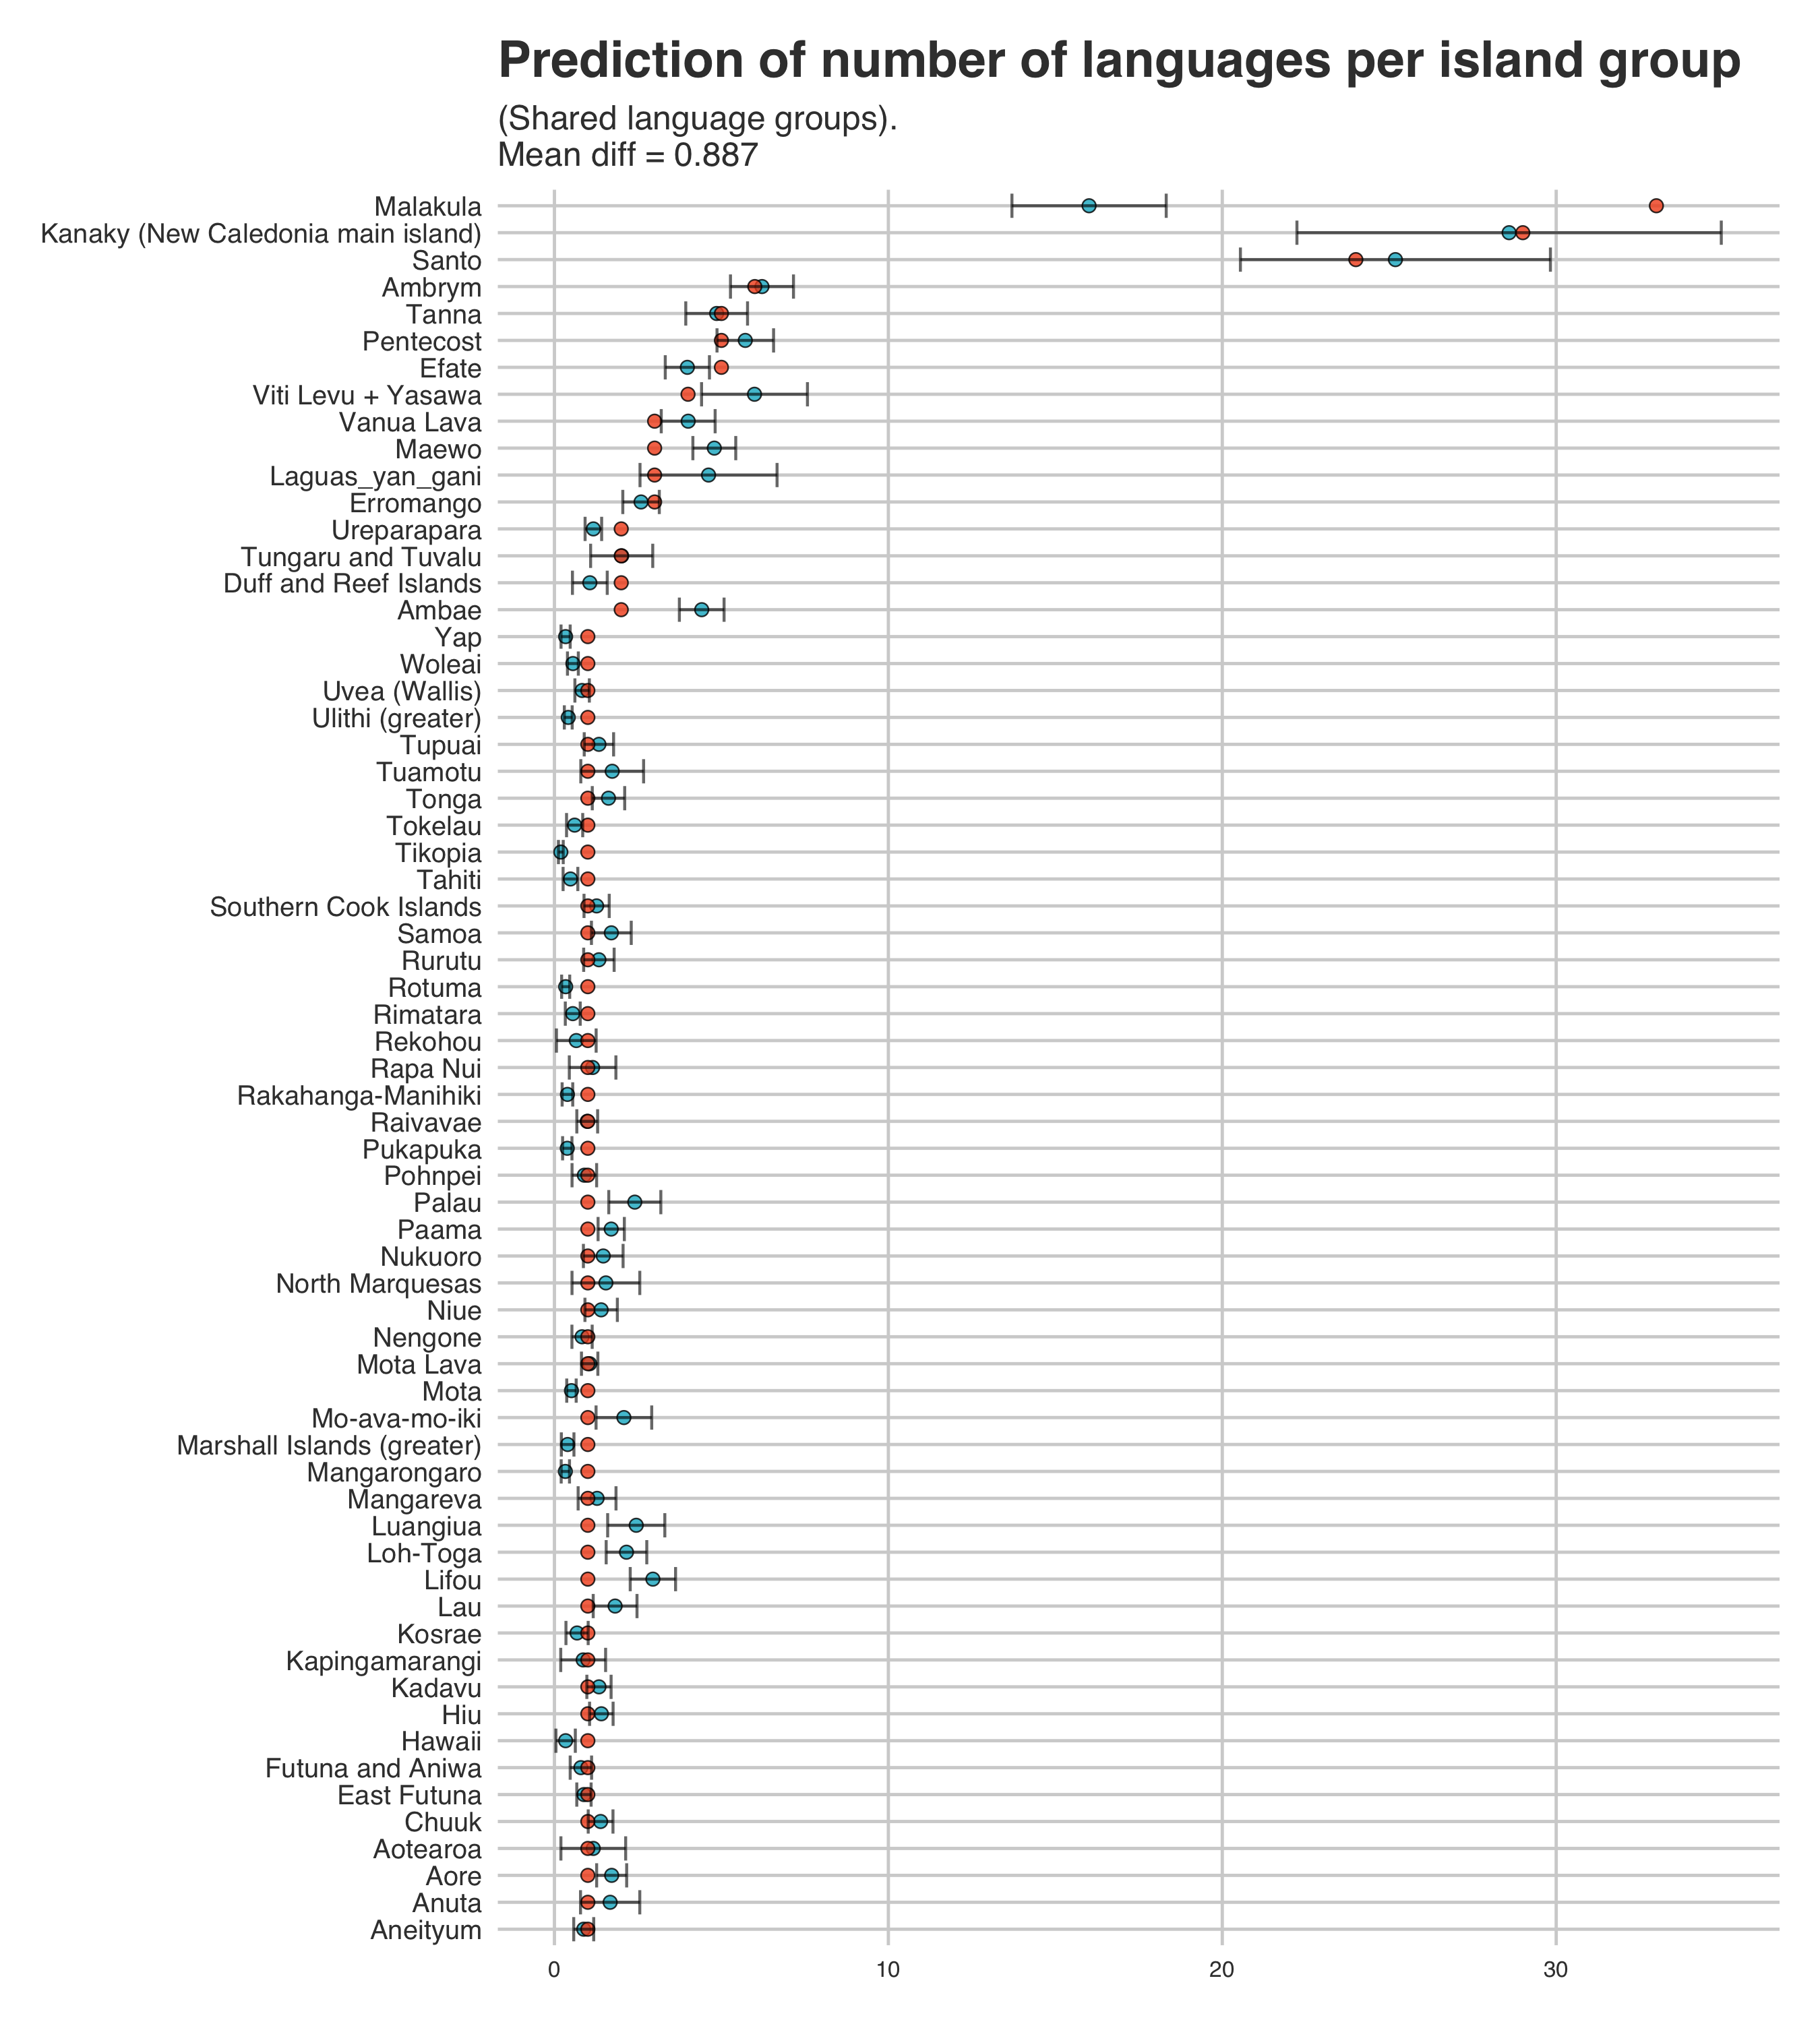
\includegraphics[width=\textwidth]{illustrations/plots_from_R/medium_group_model_prediction.png}
\caption{Untransformed values.}
    \end{subfigure}
\hfil
    \begin{subfigure}{12cm}
\centering
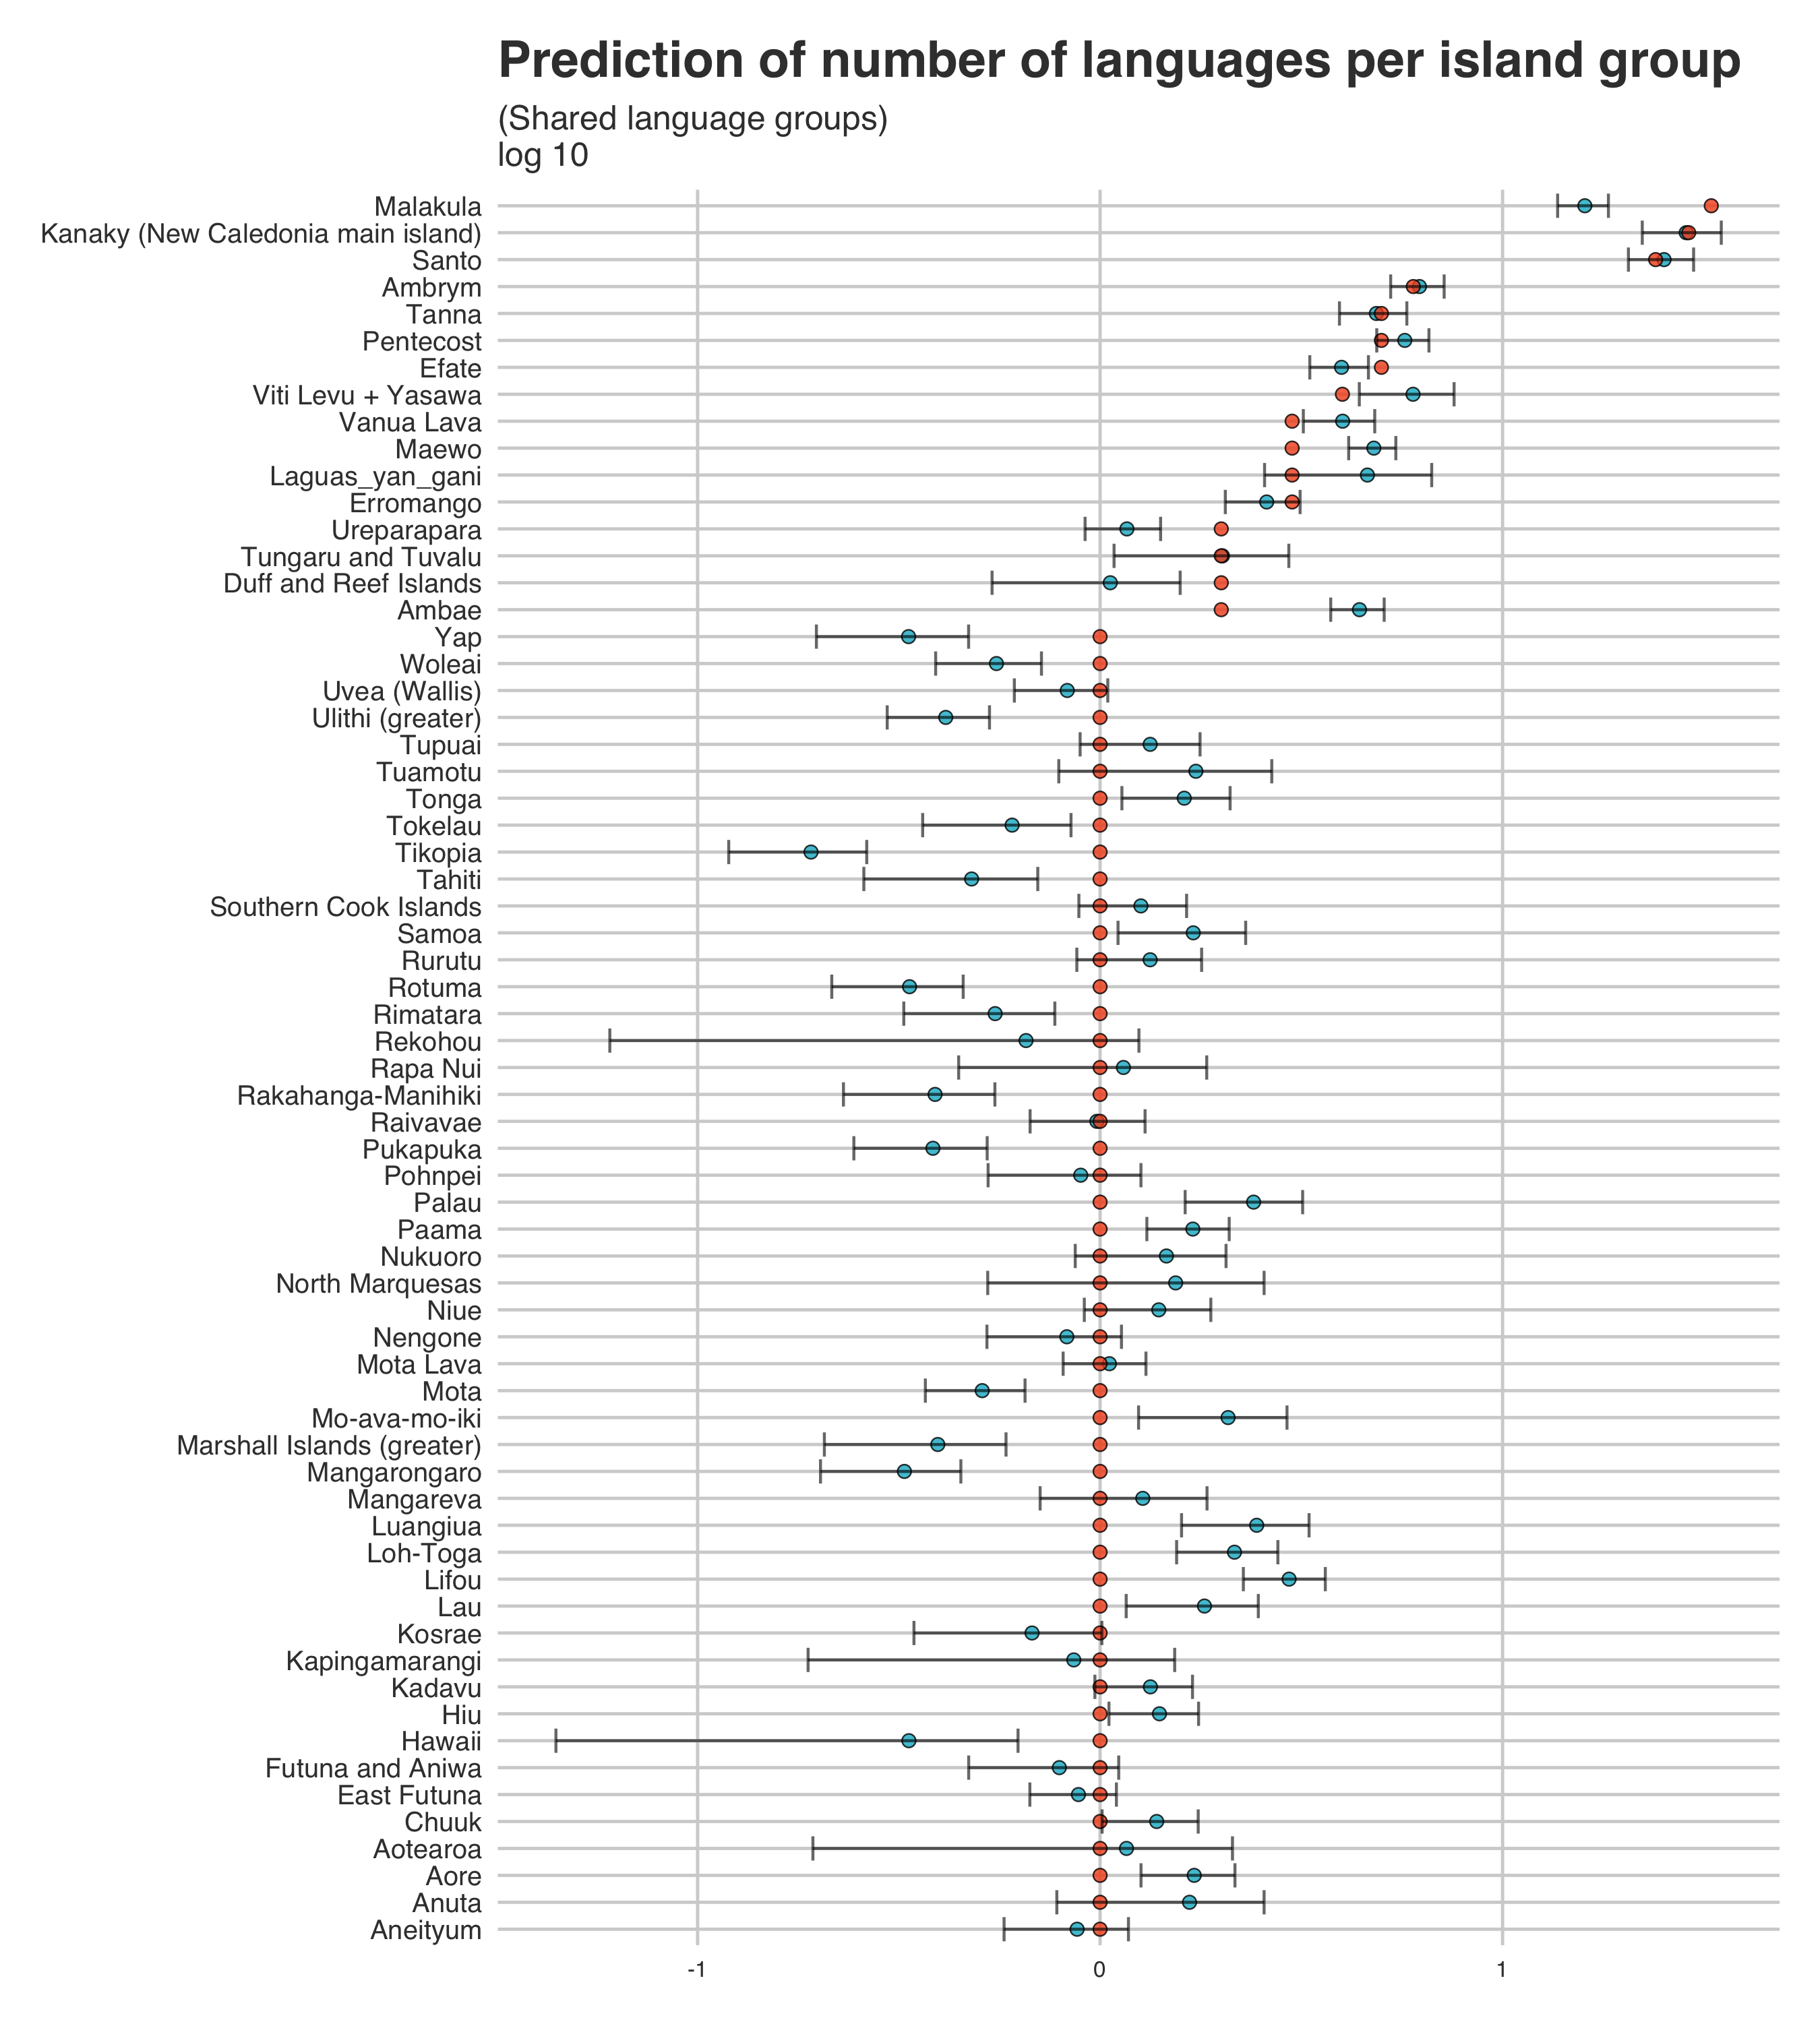
\includegraphics[width=\textwidth]{illustrations/plots_from_R/medium_group_model_prediction_log10.png}
\caption{Values transformed log-10.}
    \end{subfigure}
    \caption[Model prediction for shared language island group.]{{Model prediction for shared language island groups. Red = observed language count, blue = prediction and bars = standard error.  \emph{n}= 65}}
\label{medium_model_predict}
\end{sidewaysfigure}

%Most of the island groups in this dataset have only one language, and this seems to have caused some issues (despite the Negative Binomial distribution). The model does best at predicting languages in Polynesia (which is dominated by island groups with only one language). Islands groups in Polynesia can have a very long coastline (like the Paumotu archipelago of French Polynesia) or very short one (like Niue). There is not as much difference in shorelines between islands of Vanuatu. The model seems to have struggled with using shoreline to predict languages globally, even leading to the result that Shoreline as a standalone term comes out in the model as negatively predicting the number of languages (though not with a \emph{p} value that passes traditional thresholds of significance). 

The log-10 transformed results (Fig. \ref{medium_model_predict}) show our results in more detail. Log-10 of one (the most common language count) is 0, hence the red line in the middle. Fractions of one have a negative value after being transformed, we can for example see this in Hawai'i. The model predicted that Hawai'i has 0.33 of a language, this is why the predicted value (blue) on the log transformed plot (Fig. \ref{medium_model_predict}b) is negative. Hawai'i is the only society in the sample with a political complexity level of four, and since higher complexity leads to fewer languages in this model Hawai'i is predicted to score especially low.

%Among the island groups the model predicted \textit{least} successfully is Paama, a very small island of Vanuatu with one language. The model predicted 5.2 languages, the observer value is one. 

%Paama is coded 1 for political complexity \citep{bonnemaison1996graded} and as part of the third wave of settlement \citep{rieth_cochrane_2018}. Most island groups that are coded as low for political complexity and low for settlement are found in Vanuatu and can be somewhat differentiated by Shoreline with Malakula and Santo having longer shorelines and more languages. However, in the full sample there are island groups with much longer shorelines and only one language (Aotearoa and Paumotu). The estimates of the model show that while the interaction of Shoreline and Settlement order has a significant positive influence as an interaction, the effect is not large.

For the overnight distance groups we again see that political complexity has a significant effect predicting languages (Table \ref{table:GLM_model_marck}), however time depth in interaction with size (area) has a stronger effect.

% latex table generated in R 3.6.0 by xtable 1.8-4 package
% Sat Jan 11 13:08:09 2020
\begin{table}%[h]
\centering
\begin{tabular}{rrrrr}
  \hline
Variable & Correlation Estimate & Std. Error & Z-value & \emph{p} value \\ 
  \hline
(Intercept) & 0.18 & 0.14 & 1.28 & 0.20 \\ 
Settlement wave order:Area (log10) & 0.53 & 0.11 & 4.80 &   \textbf{<0.01} \\   
Political complexity (EA033) & -0.28 & 0.12 & -2.37 & \textbf{0.02} \\ 
Rainfall seasonality mean & -0.15 & 0.13 & -1.13 & 0.26 \\ 
Temperature seasonality mean & -0.06 & 0.14 & -0.39 & 0.70 \\ 
Shoreline (log10) & 0.20 & 0.31 & 0.64 & 0.52 \\ 
Settlement wave order & 0.09 & 0.16 & 0.55 & 0.58 \\ 
Area (log10)& 0.27 & 0.35 & 0.78 & 0.44 \\ 
 \hline
\end{tabular}
\caption[Table of factors in Negative Binomial Generalised Linear Model for predicting language counts in overnight distance groups.]{Table of factors in Negative Binomial Generalised Linear Model for predicting language counts in overnight distance groups, variables that pass the statistical significant test of \emph{p} value <0.05 in bold. McFadden-pseudo R$^2$ = 0.65.  \emph{n}= 58} 
\label{table:GLM_model_marck}
\end{table}
%. AIC = 199.82

Fig.~\ref{Marck_model_predict} illustrates the predictions of the model using overnight sailing distance groups. While it does predict 78 languages for Vanuatu \& Temotu, this is lower than the observed value of 128 which does not fall within the standard error of the predicted value.

    \begin{sidewaysfigure}
\centering
    \begin{subfigure}{12cm}
\centering
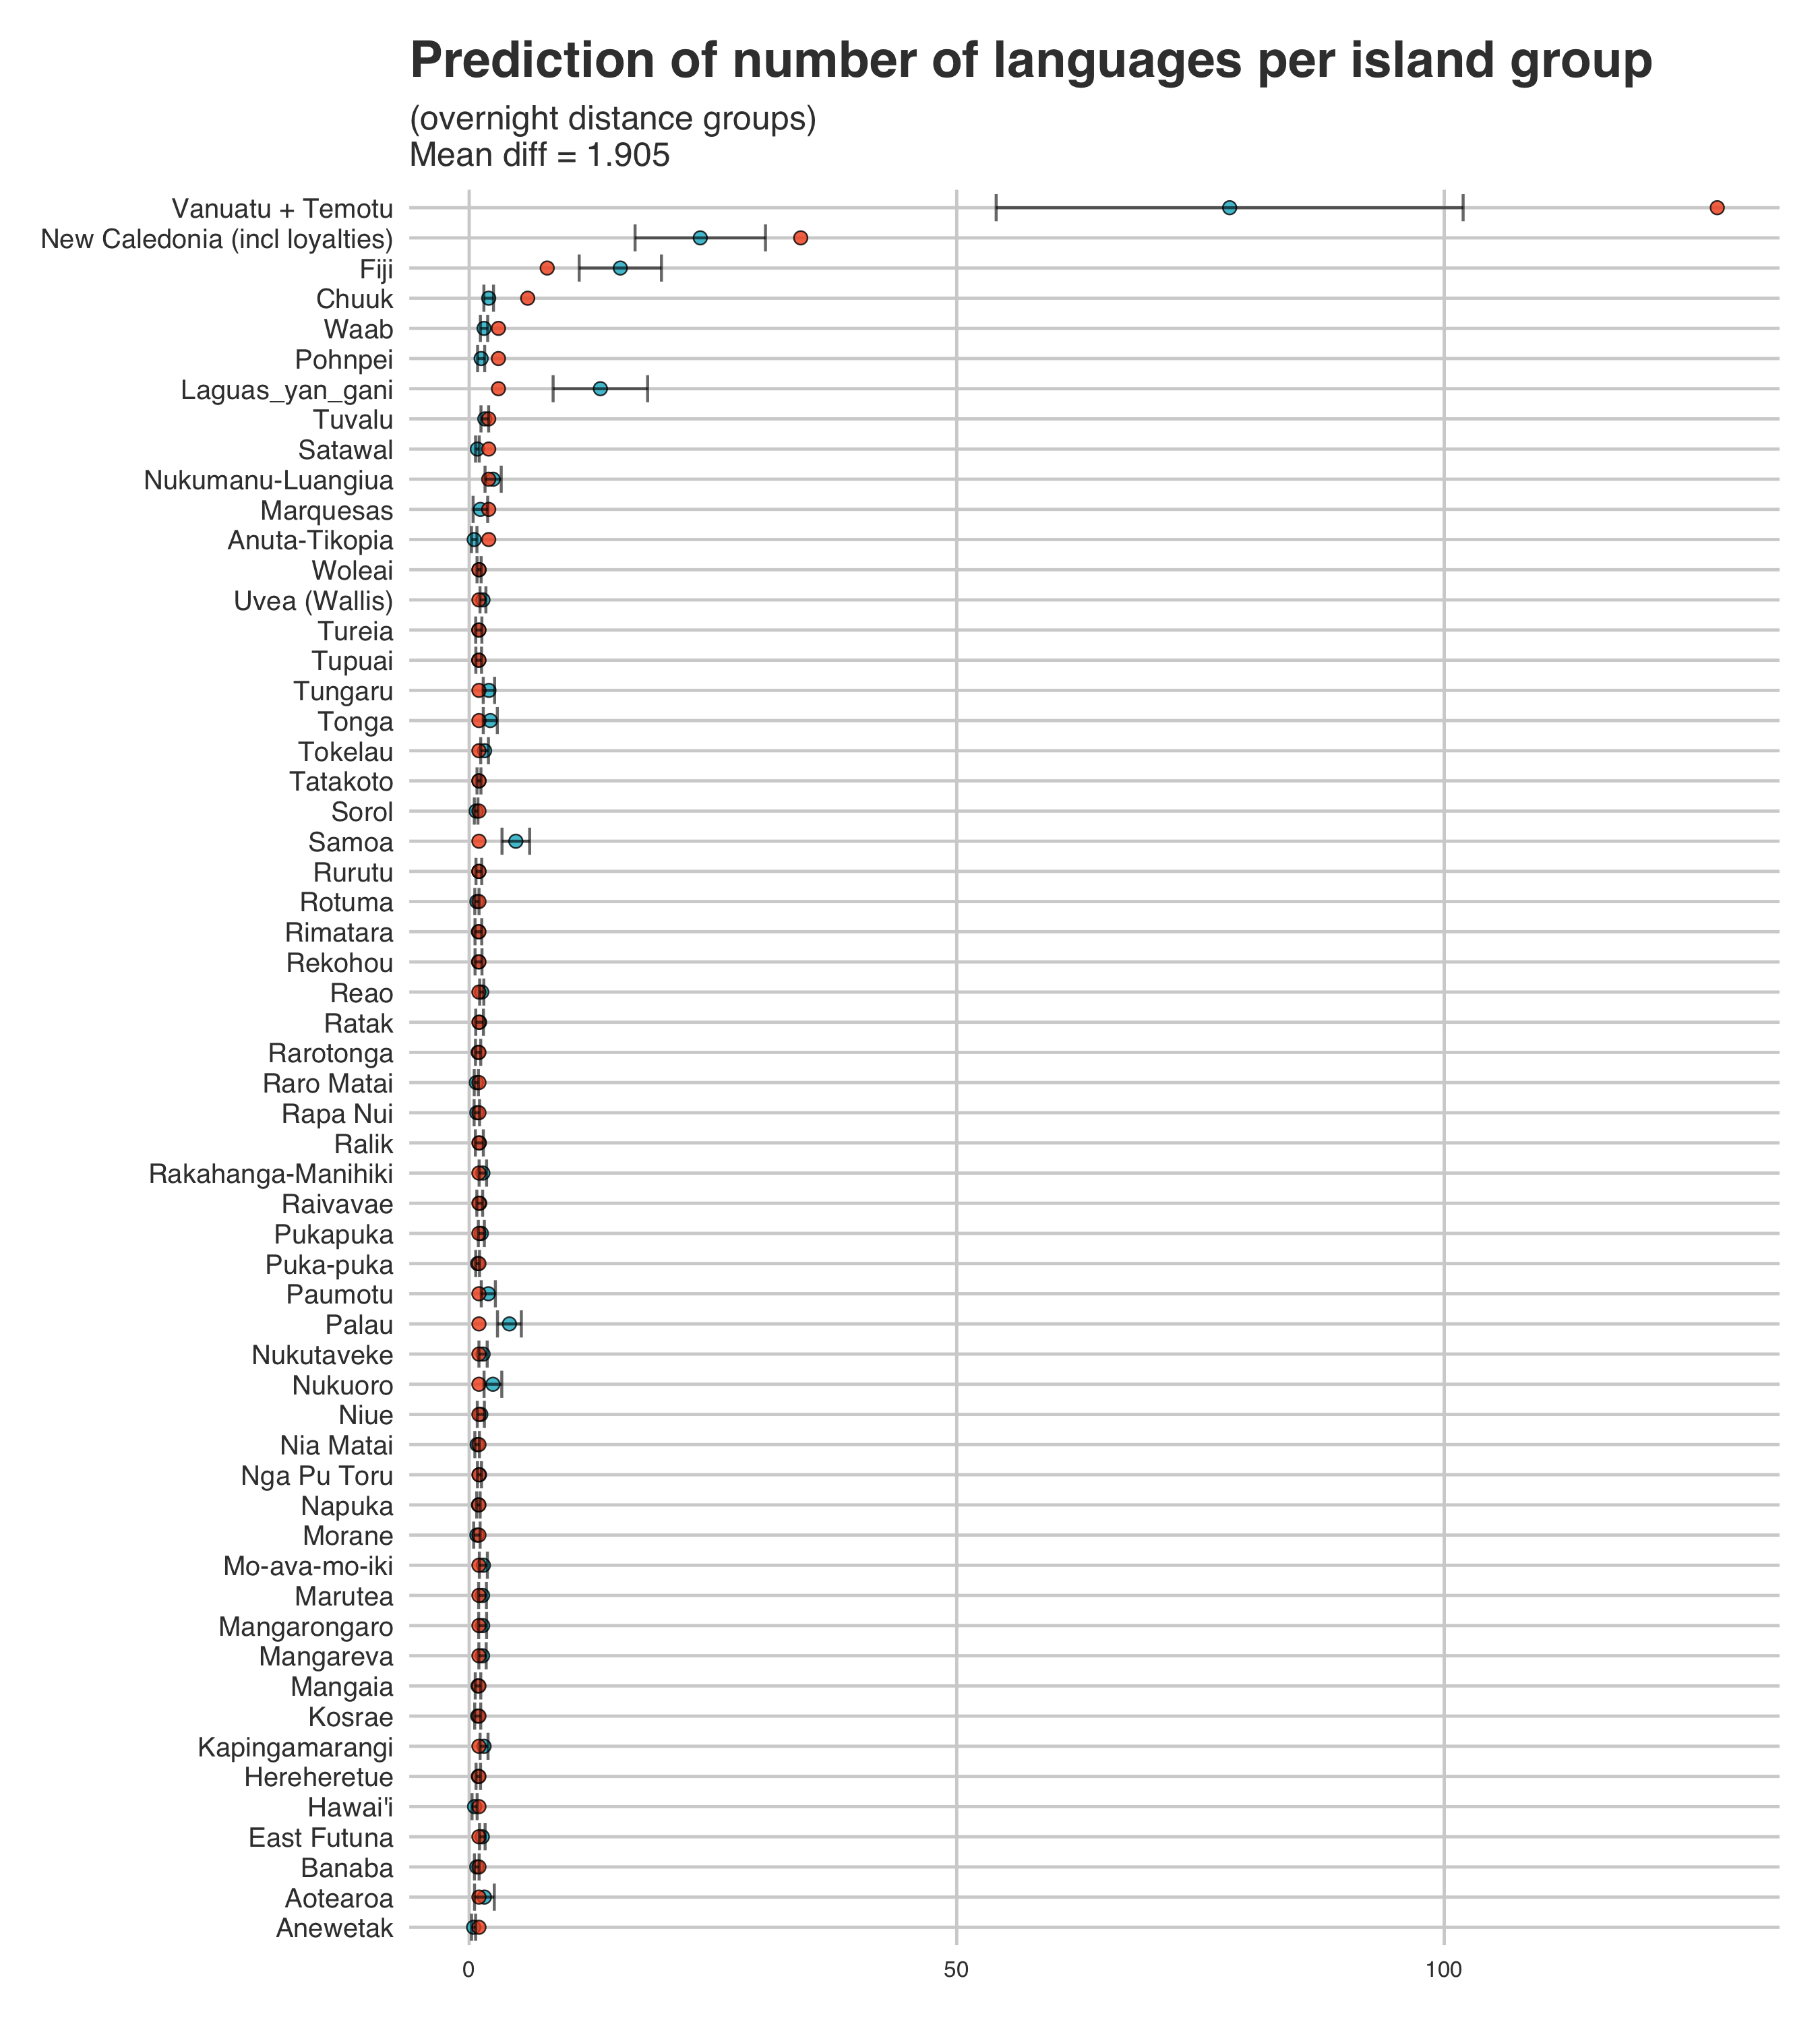
\includegraphics[width=\textwidth]{illustrations/plots_from_R/Marck_group_model_prediction.png}
\caption{Untransformed values.}
    \end{subfigure}
\hfil
    \begin{subfigure}{12cm}
\centering
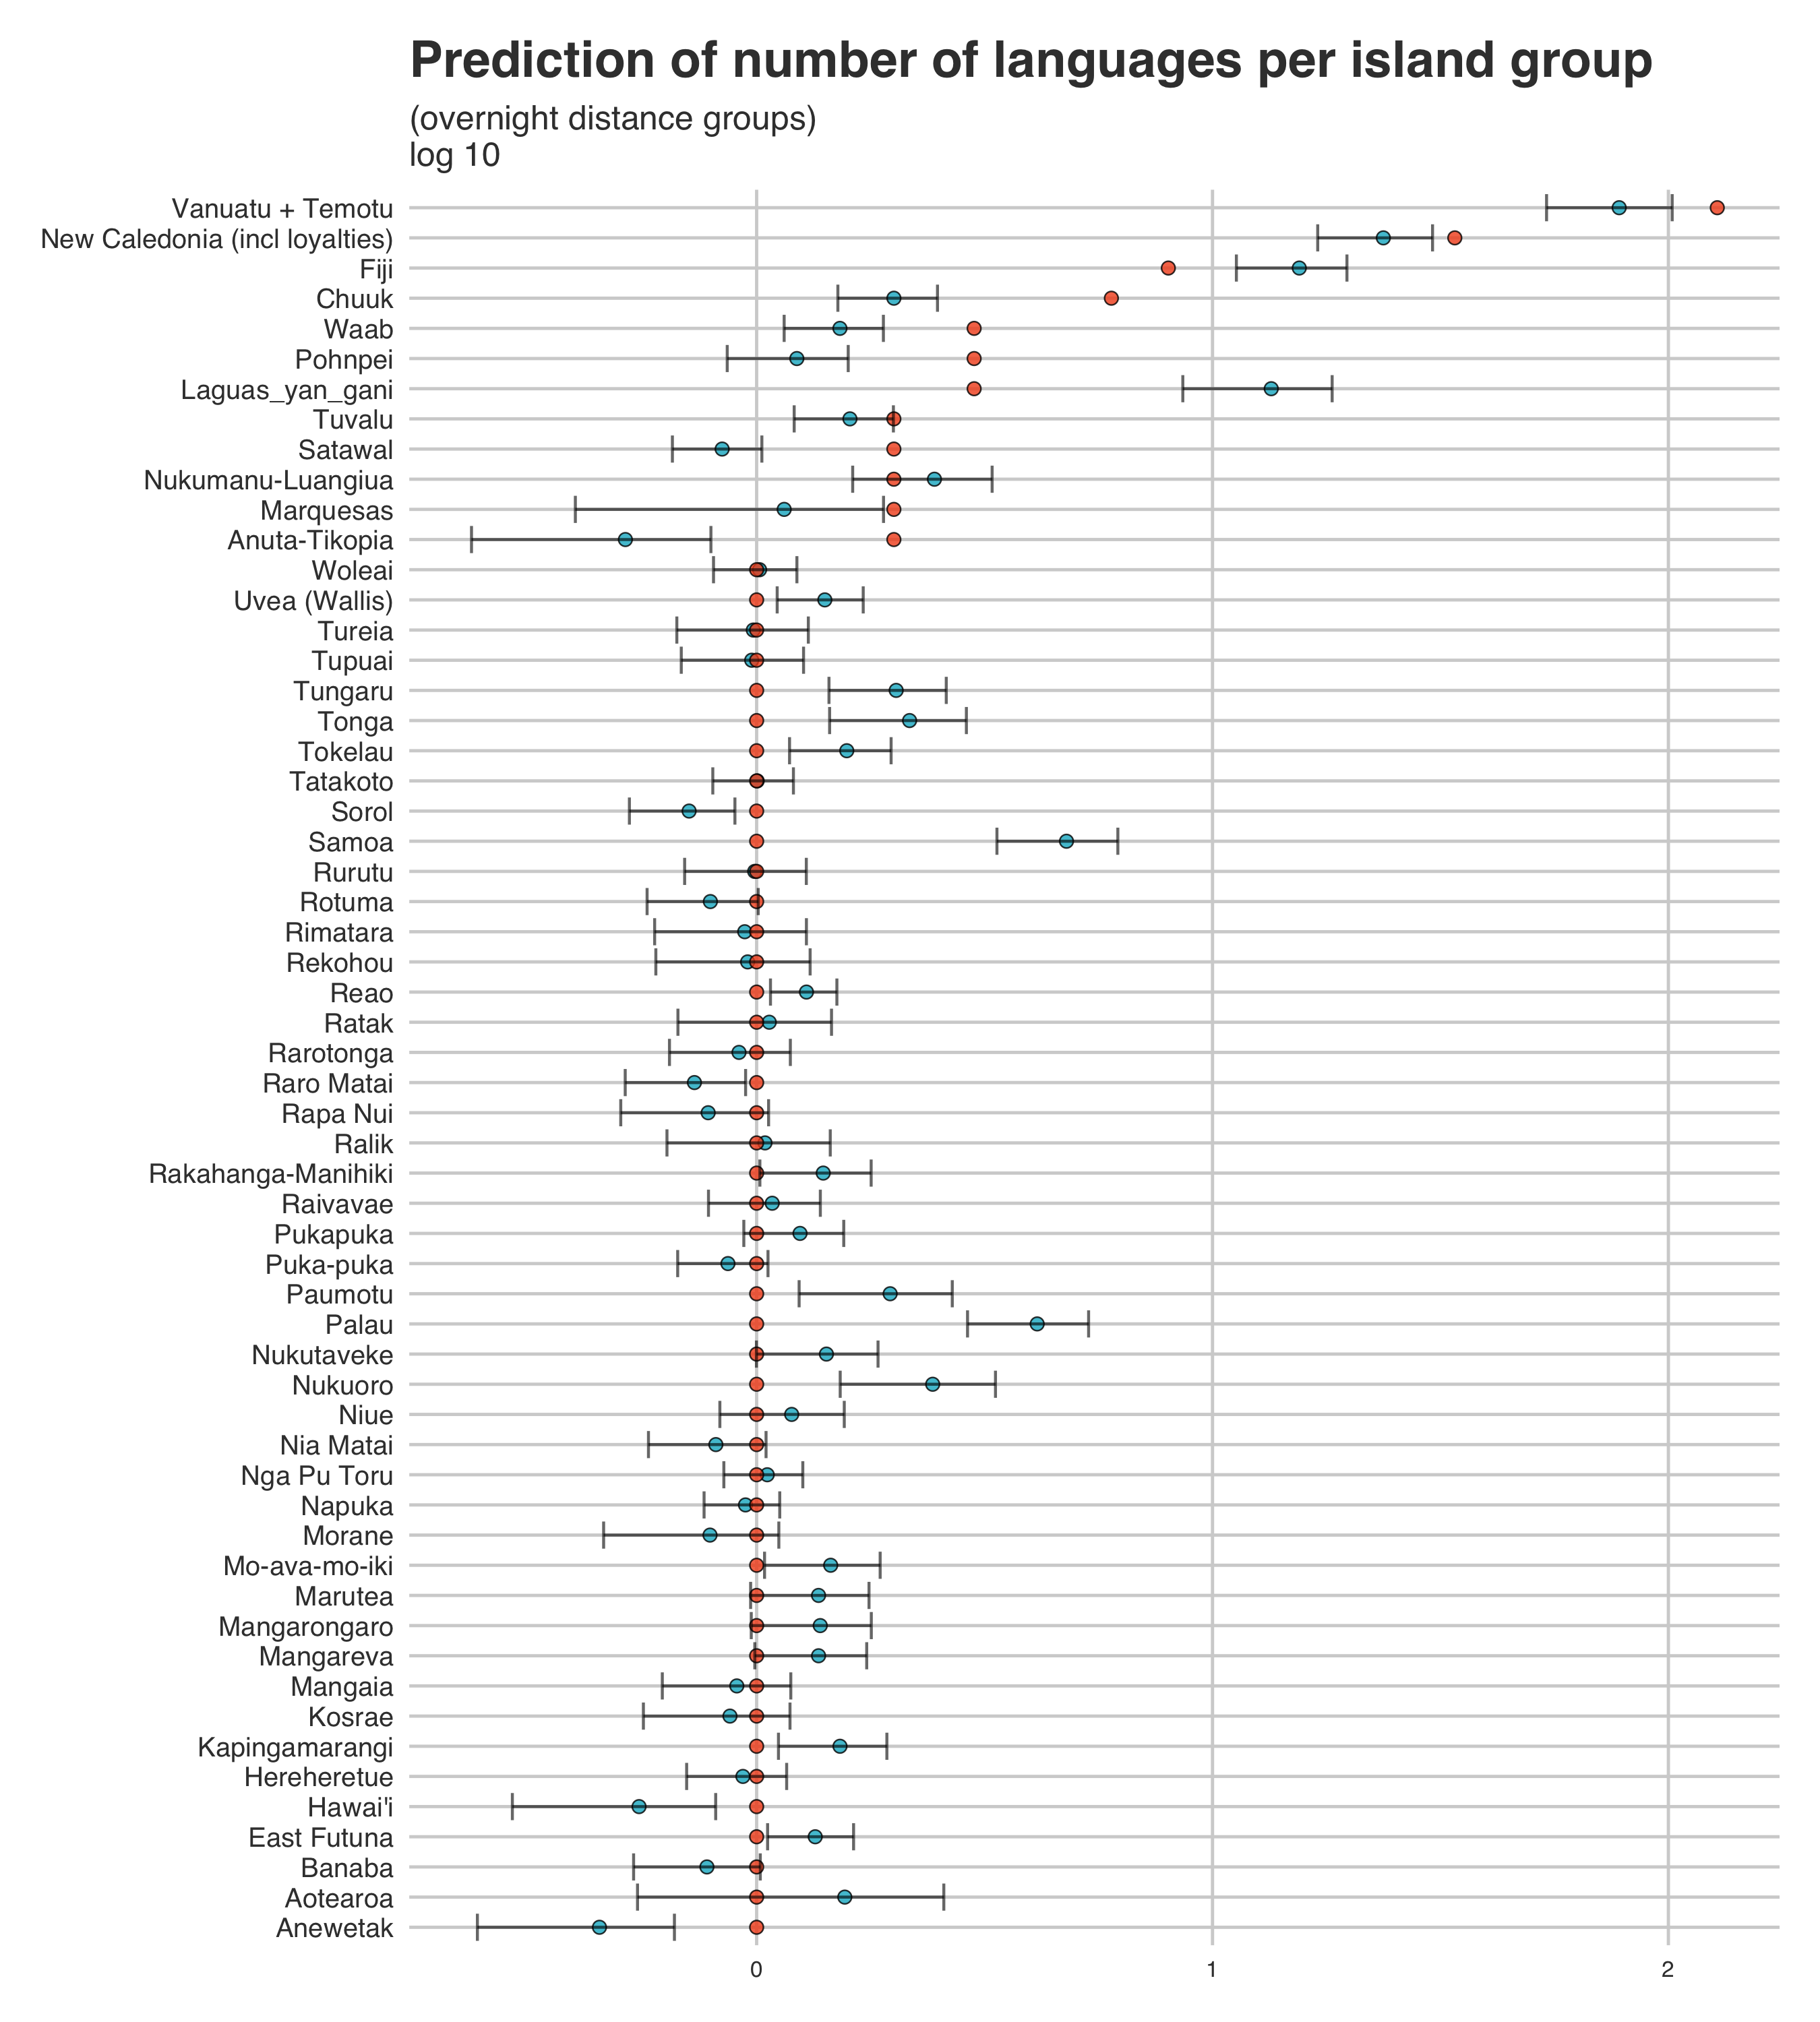
\includegraphics[width=\textwidth]{illustrations/plots_from_R/Marck_group_model_prediction_log10.png}
\caption{Values transformed log-10.}
    \end{subfigure}
\caption[Model prediction for overnight distance island groups.]{{Model prediction for overnight distance island groups. Red = observed language count, blue = prediction and bars = standard error. \emph{n}= 58}}
\label{Marck_model_predict}
\end{sidewaysfigure}


\subsection{Discussion}
\label{pol_chapter_discisson}
The results indicate that political complexity certainly is relevant for understanding the dynamics of language diversification in Remote Oceania, but further studies are needed --- especially regarding Vanuatu.

Islands of Remote Oceania were grouped in two different ways: a) by shared language(s) and b) overnight distance. The two different ways of defining island groups generated different results. The McFadden-pseudo R$^2$ \citep{mcfadden1974frontiers} for the final model of the shared language island groups is 0.56, which can be interpreted to mean that this model explains 56\% of the variance. The McFadden-pseudo R$^2$ for the overnight distance groups is even higher ---  0.65. The model with the highest pseudo R$^2$ in the work by \citet{gavin2012island} on language richness in Oceania had a value of 0.52\footnote{There are several different ways of calculating pseudo R$^2$. McFadden is widely used and recommended by \citet{allison2014measures}. The paper by \citet{gavin2012island} does not state explicitly how theirs is calculated across their various models. They use Linear Models (LM), Linear Mixed Models (LMM) and Simultaneous Autoregressive Model (SAR) --- not GLMs. I used the implementation of McFadden's pseudo-R$^2$ from the package modEvA \citep{barbosa2016package}.}. Pseudo R$^2$ scores cannot be directly compared across models and datasets, but this gives an indication that the approach and data of this chapter are on the right track.

The dataset for the overnight distance island groups contained only two island groups with significant levels of languages (New Caledonia and Vanuatu + Temotu). The model did come close to predicting the correct number of languages in New Caledonia, but it severely underestimated the number of languages in Vanuatu + Temotu (even if it did predict this group to have the highest number). The majority of the rest of the sample was one language per island group, for both island groupings. As was mentioned earlier (section \ref{pol_complex_method}), skewed data of this kind (where only a few data-points have values much different than the rest) make it difficult to apply the correct analytical methods. In the paper on language richness in Pacific islands by \cite{gavin2012island}, they applied a different methodology (transforming the response variable). It is possible that given this data (including the environmental variables, island groupings, political complexity etc), another method would be more appropriate.

Both models include political complexity as a statistically significant factor for predicting language diversity in Remote Oceania which gives support to the hypothesis tested in this chapter. As expected, space and time also came out as significant factors. This indicates that the longer time people lived in a place and the longer shoreline/more land there was, the more languages arise. This is in line with previous research. \citet{curriemace2009} found that politically complex societies (``ethnolinguistic groups'') cover a larger geographical area than societies with low political complexity.  Assuming one language per society\footnote{By using language area as a measurement of the size of ethnolinguistic groups/societies, \citet{curriemace2009} make this assumption.}, a random 10 km$^2$ sample which has a high average value for political complexity (averaging over all language polygons that are found in the cell) will then have fewer languages. For example, the language Turkish is associated with a political complexity score of four \citep{d_place_all} and covers a large area whereas the many languages of the nearby Caucasus are generally coded as low political complexity and cover smaller areas \citep{ethnologue2005}. If we take a 10 km$^2$ sample in Anatolia (where Turkish is spoken) we find fewer languages and higher complexity on average than if we sample the same sized area in the Caucasus. Similarly, we find fewer languages per island group in Remote Oceania the higher the average political complexity.

A counterexample to this trend globally is the presence of large areas covered by language-societies with low political complexity and majority pastoralist subsistence strategies. \citet{curriemace2009} found such cases, but their results concluded that the best predictor for the overall global patterns in their data was still political complexity. Another possible counterexample might be regions of many societies with high complexity where each society covers a small area in close proximity to each other. This is arguably the case for historic city states in Ancient Greece as these covered fairly small areas and had many political levels (see \citet{cartwright_2013}, and \citet[19]{sealey1976history}). However, the city states of Ancient Greece are usually all described as speaking different dialects of the same language, not different languages. This means that the language area of Ancient Greek (which is what \citet{curriemace2009} measured) would still be large and the average political complexity high, which would support their hypothesis.

\citet{curriemace2009} argue that the reason behind their results (higher political complexity = larger language areas) is that societies with higher political complexity are more likely to be able to replace existing groups in an area, or otherwise incorporate them. In his theory of language diversification in Remote Oceania, \citet{pawley2007} writes that the islands of Melanesian Remote Oceania and Western Polynesia were colonised in a similar manner but that the divergence was slowed down in West Polynesia and Fiji due to the rise of powerful political leaders who had a vested interest in the \emph{maintenance} of long distance voyaging and large scale food production. It may also be the case that diversity in Polynesia was reduced by later expansionist efforts by societies with higher political complexity. For example, the island of Niuafo'ou which lies between Tonga, 'Uvea and S\={a}moa is home to a language which is most closely related to 'Uvean. This language has however become \emph{more} similar to Tongan during the period of Tongan domination in the area 1000-1300's (see \citet{aswani1998tongan} and \citep[2-9]{tuskamoto_niuafoou}). It may be that politically complex societies do not only \emph{maintain} homogeneity by continuing being in contact after first settlement, but can also reduce diversity which emerges after settlement through incorporation and cultural dominance later.

\citet{watts_2018} found that politically complex societies in Oceania were Christianised faster. This may indicate that changes propagate through a population quicker if the society is not egalitarian. If Christianity spreads faster in societies with higher complexity, it is possible to reason that other changes also might spread faster. If changes propagate quickly throughout a population, that leaves less possibility for diversification through natural drift or groups in the periphery staying more archaic compared to the centre. This interpretation relies on the understanding that the variable for political complexity (EA033) reveals something not only about jurisdictional power relationships in a given society, but also captures something about the social network of \emph{all} of its members (not just the leaders). Under this theory, people living in societies with higher political complexity would be able to travel further and have wider ranging social networks, which in turn would lead to greater internal cultural homogeneity.

It should also be noted that these preliminary results do not answer the question why Melanesian Remote Oceanic societies are indeed less politically complex. Nor do they disprove the hypothesis that there are more languages in Melanesian Remote Oceania because of influence from non-Austronesian migrants (c.f. \citet{lynch1981melanesian}). It is possible that there are more languages \emph{and} lower political complexity because of non-Austronesian contact but that these two variables are not actually related to \emph{each other} (c.f. Galton's problem \citep{naroll1965galton}). 

%It is beyond the scope of this study to fully investigate the causality of language diversification in Remote Oceania. Causality in cultural evolution is very complicated, since factors can interact on many levels and it is difficult to control for unknown variables and proxy effects (c.f \citet{roberts2013linguistic}). In this instance, we will be satisfied with testing if there is a correlation between societal structure and language diversity that is still signifncant once environmental and settlement time has been incorporated into the model.

Unlike the studies by \citet{gavin2012island}, \citet{hua2019ecological} and others, these results indicate that environmental factors such as rainfall seasonality and isolation have less of an impact on language diversity in Remote Oceania. The variables that have a significant effect are size (area and shoreline), time depth and political complexity. The fact that the results did not find that variables which have been predictive elsewhere have an impact in these models should not be taken as conclusive and may be due to limitations of this particular work.

%As can be seen from the specific predictions the models make (Fig. \ref{medium_model_predict} and Fig. \ref{Marck_model_predict}), neither model accurately predicts the key island groups in our dataset (Vanuatu, Kanaky (New Caledonia) and Temotu). Explaining the difference between Melanesian Remote Oceania and the rest is the most important factor in evaluating our hypothesis. Therefore the results should be interpreted as ultimately inconclusive. 

\citet{Pacheco_Coelho_2019} explore an approach where the predictive power of each variable is not fixed, but changes with respect to location. Such an approach may give more insight into this dataset, and is left as future work.

Possible limitations with this chapter are: a) the way that islands groups are defined, b) the manner in which the over-dispersion was accounted for and c) poor measurements of, or missing, key variables. Concerning (a), it may be that a grid-approach (c.f \citet{hua2019ecological}) is more appropriate. One of the problems with a grid approach is that it may work less well in an oceanic environment where connections between islands are not accounted for appropriately, but it should be tested in a similar manner to this chapter to evaluate if this indeed is a problem. A more finer grained approach similar to  \citet{gavin2012island} where each landmass is the unit of analysis may also be interesting. Both of these approaches may also aid with (b). There are other ways of accounting for (b), over-dispersion in data, besides a Negative Binomial distribution. For example, \citet[4-5]{gavin2012island} used the reciprocal of the language count. Regarding (c), \citet[4-5]{gavin2012island} found that Isolation was a significant variable in their models for predicting language diversity on Oceania (including Near Oceania). It is possible that the manner in which isolation was calculated here was suboptimal and that one or several of the other measurements of Isolation is more appropriate (see section \ref{sec:island_geo}). It was also not possible to include measurements of non-Austronesian contact in this chapter due to poor data coverage despite the fact that it could be a relevant factor (c.f. \citet{lipson_harvad_ancient_dna_vanuatu_2018, posth_jena_ancient_dna_vanuatu_2018}). 
 


\subsection{Conclusions}
This chapter investigated the hypothesis that besides time depth and environmental factors, the distribution of languages in Remote Oceania is also significantly influenced by interaction patterns that can be measured by political complexity (c.f. \citet{pawley81, pawley2007}). In order to test this hypothesis, data was gathered on rainfall, temperature, settlement date, shoreline, isolation, latitude, area, and political complexity for island groups in Remote Oceania (c.f. \citet{curriemace2009, gavin2012island, hua2019ecological} and \citet{Pacheco_Coelho_2019}). The hypothesis was tested using a Negative Binomial Generalised Linear Model and stepwise dropping variables given an ANOVA Chi-square test.

The results of this chapter lend support to the theory that political complexity is a significant factor in predicting language diversity in Remote Oceania beyond what can be accounted for by environmental factors. Due to failed predictions for key regions (Vanuatu in particular), and other methodological limitations, this hypothesis needs to be investigated in future research. It appears that there is still much left to understand about language diversification in the region, and in Vanuatu in particular.

Future studies should use a grid and/or otherwise more fine grained approach to sampling, test different statistical methods that deal with over-dispersed data, and attempt to include better data on isolation, population and non-Austronesian contact. This chapter concentrated on the number of languages in a place, but it may also be revealing to include measurements of how different the languages are from each other, in lexicon and/or structure.

In the next chapter we explore the disparity of languages of Remote Oceania, how different they are from each other.

%Linking chapter 2 to chapter 3
%In chapter 2 we show that yes internal structure of a community is a factor, that means that the variation within a community can be linked to overall change between communities. In the next chapter we will look into more detail the way that linguists have approached these two levels of variation, micro and macro.


\newpage



\newpage
\singlespacing
\bibliographystyle{unified_edit_HS_SFM}
\bibliography{hsz_out}
%\singlespacing


\newpage
\singlespacing
\appendix
\section*{Appendices}
\addcontentsline{toc}{section}{Appendices}
\renewcommand{\thesubsection}{\Alph{subsection}}



\subsection{Table of Political complexity scores per society}
\label{Pol_complex_table}
\singlespacing
The political complexity scores are based on \cite{sheehan2018coevolution}, the Ethnographic Atlas  \citep{d_place_all},\citet{bonnemaison1972systeme} and \cite{bonnemaison1996graded}. The scores from  \cite{sheehan2018coevolution} and the Ethnographic Atlas are displayed along with the score used in chapter \ref{chapter_pol_complex}. I re-evaluated the scores and inspected the references again to come to an independent decision, this is why the scores sometimes differ.

In the study by \cite{sheehan2018coevolution} they make a distinction which between 0 = local communities are associations of households (or other sub-local groups, such as village wards) with no overarching system of authority and 1 = autonomous local communities which each had a system of authority, e.g. a village council (Sheehan personal correspondence). These two levels are merged in my coding and the coding from the Ethnographic Atlas. \emph{NA} stands for missing data.

\begin{landscape}
\begin{longtable}{ | p{2cm}| p{2cm}| p{1.8cm}| p{1.8cm}| p{3cm}| p{9cm}| }

\caption{{Table of Political Complexity score per society}} 
\label{pol_complex_table}\\
\hline
\multirow{2}{*}{\parbox{2cm}{\textbf{Language name}}} &\multirow{2}{*}{\textbf{Glottocode}}&  \multicolumn{3}{p{6.6cm}|}{\textbf{Political Complexity (EA033)}} & \multirow{2}{*}{\textbf{References}} \\ \cline{3-5}
&& \textbf{This thesis}& \textbf{Sheehan et al 2008}& \textbf{Ethnographic Atlas (D-PLACE)}&\\ \hline




\endfirsthead

%\caption[]{\textbf{Table of settlement date per island group based on archaeology}} \\
\hline
\multirow{2}{*}{\parbox{2cm}{\textbf{Language name}}} &\multirow{2}{*}{\textbf{Glottocode}}&  \multicolumn{3}{p{6.6cm}|}{\textbf{Political Complexity (EA033)}} & \multirow{2}{*}{\textbf{References}} \\ \cline{3-5}
&& \textbf{This thesis}& \textbf{Sheehan et al 2008}& \textbf{Ethnographic Atlas (D-PLACE)}&\\ \hline

\endhead

\hline
East Ambae&east2443&1&\emph{NA}&1&Bonnemaison, J. (1972). Système de grades et diff\'{e}rences r\'{e}gionales en Aoba (Nouvelles H\'{e}brides). Cahiers ORSTOM. S\'{e}rie Sciences Humaines, 9(1), 87-108.\\ \hline
West Ambae&west2513&1&\emph{NA}&1&Bonnemaison, J. (1972). Système de grades et diff\'{e}rences r\'{e}gionales en Aoba (Nouvelles H\'{e}brides). Cahiers ORSTOM. S\'{e}rie Sciences Humaines, 9(1), 87-108.\\ \hline
Southeast Ambrym&sout2859&1&1&\emph{NA}&Tonkinson R (1981) Church and Kastom in Southeast Ambrym. Vanuatu: Politics, Economics and Ritual in Island Melanesia, ed Allen M (Academic Press, Sydney, Australia), pp 237-267.\\ \hline
Aneityum&anei1239&2&2&\emph{NA}&Humphreys CB (1926) Southern New Hebrides: An Ethnological Record (Cambridge Univ Press, Cambridge, UK); Spriggs M (1982) Taro Cropping Systems in the Southeast Asian-Pacific Region: Archaeological Evidence. Archaeol Ocean 17(1):7-15; Spriggs M (1986) Landscape, Land Use, and Political Transformation in Southern Melanesia. Island Societies: Archaeological Approaches to Evolution and Transformation, ed Kirch PV (Cambridge Univ Press, New York, NY), pp 6-19. \\ \hline
Anuta&anut1237&1&1&\emph{NA}&Feinberg R (1988) Socio-Spatial Symbolism and the Logic of Rank on Two Polynesian Outliers. Ethnology 27(3):291-310; Feinberg R (1991) Anuta. Encyclopaedia of World Cultures (Vol II: Oceania) (G.K. Hall and Co, New York, NY), pp 13-16.; Kirch PV (2002) Te Kai Paka-Anuta: Food in a Polynesian Outlier Society. Le Journal de la Soci\'{e}t\'{e} des Oc\'{e}anistes 114-115:71-89. \\ \hline
Aore&aore1237&1&\emph{NA}&\emph{NA}&Bonnemaison, J (1996) The Art of Power. In Bonnemaison (eds) Arts of Vanuatu. University of Hawaii Press.\\ \hline
Rennell-Bellona/Mu-Ngava-Mu-Hgiki&renn1242&2&2&2&Birket-Smith K (1969) An Ethnological Sketch of Rennell Island, a Polynesian Outlier in Melanesia (2nd Ed) (Bianco Lunos Bogtrykkeri, Copenhagen, Denmark); Monberg T (1991) Bellona Island Beliefs and Rituals (Univ Hawaii Press, Honolulu, HI). \\ \hline
Chuukese&chuu1238&2&2&1&Goodenough WH (1991) Truk. Encyclopaedia of World Cultures (Vol II: Oceania) (G.K. Hall and Co, New York, NY), pp 351-354; Goodenough WH (2002) Under Heaven's Brow: Pre-Christian Religious Tradition in Chuuk (American Philosopical Society, Philadelphia, PA); (1960) Taro cultivation in Truk. Taro Cultivation Practices and Beliefs: Part II. The Eastern Carolines and the Marshall Islands, ed Young JE (Office of the Staff Anthropologist, Guam, GU), pp 70-98. \\ \hline
East Futuna&east2447&2&2&2&Kirch PV (1994) The Wet and the Dry: Irrigation and Agricultural Intensification in Polynesia (Univ Chicago Press, Chicago, IL);\\ \hline
North Efate&nort2836&2&2&\emph{NA}&Facey EE (1981) Hereditary chiefship in Nguna. Vanuatu: Politics, Economics and Ritual in Island Melanesia, ed Allen M (Academic Press, Sydney, Australia), pp 295-314. Facey EE (1991) Nguna. Encyclopaedia of World Cultures (Vol II: Oceania) (G.K. Hall and Co, New York, NY), pp 242-244. \\ \hline
Sie&siee1239&2&2&\emph{NA}&Humphreys CB (1926) Southern New Hebrides: An Ethnological Record (Cambridge Univ Press, Cambridge, UK). Spriggs M, Wickler S (1989) Archaeological Research on Erromango: Recent Data on Southern Melanesian Prehistory. Bulletin of the Indo-Pacific Prehistory Association 9:68-91.\\ \hline
Futuna-Aniwa&futu1245&2&2&\emph{NA}&Capell A (1958) Culture and Language of Futuna and Aniwa, New Hebrides (Univ Sydney, Sydney, Australia).\\ \hline
Chamorro&cham1312&1&1&2&Cordy R (1983) Social stratification in the Mariana Islands. Oceania 53(3):272-276; Thompson L (1971) The Native Culture of the Marianas Islands (Bernice P Bishop Museum Bulletin, Honolulu, HI) (Originally published 1945). \\ \hline
Hawaiian&hawa1245&4&4&3&Kirch PV (1994) The Wet and the Dry: Irrigation and Agricultural Intensification in Polynesia (Univ Chicago Press, Chicago, IL). Kirch PV (2010) How Chiefs Became Kings: Divine Kingship and the Rise of Archaic States in Ancient Hawai'i (Univ California Press, Oakland, CA).\\ \hline
Hiw&hiww1237&1&\emph{NA}&\emph{NA}&Bonnemaison, J (1996) The Art of Power. In Bonnemaison (eds) Arts of Vanuatu. University of Hawaii Press.\\ \hline
Fijian&fiji1243&3&3&\emph{NA}&Kuhlken R (2002) Intensive Agricultural Landscapes of Oceania. Journal of Cultural Geography 19(2):161-195. 80) Scarr D (1984) Fiji: A Short History (George Allen and Unwin, Sydney, Australia). 81) Walter MAHB (1978) An examination of hierarchical notions in Fijian society: A test case for the applicability of the term ‘chief’. Oceania 49(1):1-19. \\ \hline
Ajië&ajie1238&1&\emph{NA}&2&Winslow, Don (1991) Ajie. Encyclopaedia of World Cultures (Vol II: Oceania) (G.K. Hall and Co, New York, NY), pp 9.\\ \hline
Xârâcùù&xara1244&3&3&\emph{NA}&Young MW (1991) Goodenough Island. Encyclopaedia of World Cultures (Vol II: Oceania) (G.K. Hall and Co, New York, NY), pp 85-88.\\ \hline
Kapingamarangi&kapi1249&1&1&2&Buck PH (1950) Material Culture of Kapingamarangi (Bernice P. Bishop Museum, Honolulu, HI). Emory KP (1965) Kapingamarangi: Social and Religious Life of a Polynesian Atoll (The Museum, Honolulu, HI). \\ \hline
Kosraean&kosr1238&3&3&3&Athens JS (2007) Prehistoric Population Growth on Kosrae, Eastern Caroline Islands. The Growth and Collapse of Pacific Island Societies, eds Kirch PV, Rallu J (Univ Hawaii Press, Honolulu, HI), pp 257-277. Graves MW (1986) Late Prehistoric Complexity on Lelū: Alternatives to Cordy’s Model. J Polyn Soc 95(4), 479-489. Peoples JG (1991) Kosrae. Encyclopaedia of World Cultures (Vol II: Oceania) (G.K. Hall and Co, New York, NY), pp 128-131. \\ \hline
Lauan&laua1243&3&0&3&Hocart, A. M. 1929. Lau Islands, Fiji. (Bull. Bishop Mus., 62.) 1-240pp. Quain, Buell H. 1948. Fijian village. Chicago: University of Chicago Press. Thompson, L. 1940. Southern Lau, Fiji. (Bull. Bishop Mus., 162.) Thompson, Laura. 1940. Fijian frontier. (Studies of the Pacific.) San Francisco: Institute of Pacific Relations.\\ \hline
Dehu&dehu1237&2&\emph{NA}&2&Hadfield, E. 1920. Among the Natives of the Loyalty Group., Ray, S. 1917. The People and Language of Lifu, Loyalty Islands. Journ. Roy. Anth. Inst. 47. 239-322.\\ \hline
Äiwoo&ayiw1239&1&0&\emph{NA}&Davenport WH (1969) Social organization notes on the Northern Santa Cruz Islands: the Main Reef Islands. Baessler-Archiv, Neue Folge 17(1):151-243.\\ \hline
Luangiua&onto1237&1&1&1&Sahlins MD (1958) Social Stratification in Polynesia (Univ Washington Press, Seattle, WA). Bayliss-Smith T (1974) Constraints on population growth: The case of the Polynesian Outlier atolls in the precontact period. Hum Ecol 2(4):259-295. Donner WW (1991) Ontong Java. Encyclopaedia of World Cultures (Vol II: Oceania) (G.K. Hall and Co, New York, NY), pp 253-255. \\ \hline
Baetora&baet1237&1&\emph{NA}&\emph{NA}&Bonnemaison, J (1996) The Art of Power. In Bonnemaison (eds) Arts of Vanuatu. University of Hawaii Press.\\ \hline
Central Maewo&cent2058&1&\emph{NA}&\emph{NA}&Bonnemaison, J (1996) The Art of Power. In Bonnemaison (eds) Arts of Vanuatu. University of Hawaii Press.\\ \hline
Sunwadia&mari1426&1&\emph{NA}&\emph{NA}&Bonnemaison, J (1996) The Art of Power. In Bonnemaison (eds) Arts of Vanuatu. University of Hawaii Press.\\ \hline
Aulua&aulu1238&1&\emph{NA}&\emph{NA}&Bonnemaison, J (1996) The Art of Power. In Bonnemaison (eds) Arts of Vanuatu. University of Hawaii Press.\\ \hline
Avok&avok1244&1&\emph{NA}&\emph{NA}&Bonnemaison, J (1996) The Art of Power. In Bonnemaison (eds) Arts of Vanuatu. University of Hawaii Press.\\ \hline
Axamb&axam1237&1&\emph{NA}&\emph{NA}&Bonnemaison, J (1996) The Art of Power. In Bonnemaison (eds) Arts of Vanuatu. University of Hawaii Press.\\ \hline
Big Nambas&bign1238&1&\emph{NA}&\emph{NA}&Bonnemaison, J (1996) The Art of Power. In Bonnemaison (eds) Arts of Vanuatu. University of Hawaii Press.\\ \hline
Burmbar&burm1263&1&\emph{NA}&\emph{NA}&Bonnemaison, J (1996) The Art of Power. In Bonnemaison (eds) Arts of Vanuatu. University of Hawaii Press.\\ \hline
Bwenelang&bwen1239&1&\emph{NA}&\emph{NA}&Bonnemaison, J (1996) The Art of Power. In Bonnemaison (eds) Arts of Vanuatu. University of Hawaii Press.\\ \hline
Dixon Reef&dixo1238&1&\emph{NA}&\emph{NA}&Bonnemaison, J (1996) The Art of Power. In Bonnemaison (eds) Arts of Vanuatu. University of Hawaii Press.\\ \hline
Avava&katb1237&1&\emph{NA}&\emph{NA}&Bonnemaison, J (1996) The Art of Power. In Bonnemaison (eds) Arts of Vanuatu. University of Hawaii Press.\\ \hline
Ninde&labo1244&1&\emph{NA}&\emph{NA}&Bonnemaison, J (1996) The Art of Power. In Bonnemaison (eds) Arts of Vanuatu. University of Hawaii Press.\\ \hline
Larevat&lare1249&1&\emph{NA}&\emph{NA}&Bonnemaison, J (1996) The Art of Power. In Bonnemaison (eds) Arts of Vanuatu. University of Hawaii Press.\\ \hline
Letemboi-Repanbitip&lete1241&1&\emph{NA}&\emph{NA}&Bonnemaison, J (1996) The Art of Power. In Bonnemaison (eds) Arts of Vanuatu. University of Hawaii Press.\\ \hline
Neverver&ling1265&1&\emph{NA}&\emph{NA}&Bonnemaison, J (1996) The Art of Power. In Bonnemaison (eds) Arts of Vanuatu. University of Hawaii Press.\\ \hline
Naman&litz1237&1&\emph{NA}&\emph{NA}&Bonnemaison, J (1996) The Art of Power. In Bonnemaison (eds) Arts of Vanuatu. University of Hawaii Press.\\ \hline
Tirax&maee1241&1&\emph{NA}&\emph{NA}&Bonnemaison, J (1996) The Art of Power. In Bonnemaison (eds) Arts of Vanuatu. University of Hawaii Press.\\ \hline
Na'ahai&malf1237&1&\emph{NA}&\emph{NA}&Bonnemaison, J (1996) The Art of Power. In Bonnemaison (eds) Arts of Vanuatu. University of Hawaii Press.\\ \hline
Malua Bay&malu1245&1&\emph{NA}&\emph{NA}&Bonnemaison, J (1996) The Art of Power. In Bonnemaison (eds) Arts of Vanuatu. University of Hawaii Press.\\ \hline
Maragus&mara1399&1&\emph{NA}&\emph{NA}&Bonnemaison, J (1996) The Art of Power. In Bonnemaison (eds) Arts of Vanuatu. University of Hawaii Press.\\ \hline
Maskelynes&mask1242&1&\emph{NA}&\emph{NA}&Bonnemaison, J (1996) The Art of Power. In Bonnemaison (eds) Arts of Vanuatu. University of Hawaii Press.\\ \hline
Mpotovoro&mpot1241&1&\emph{NA}&\emph{NA}&Bonnemaison, J (1996) The Art of Power. In Bonnemaison (eds) Arts of Vanuatu. University of Hawaii Press.\\ \hline
Nese&nese1235&1&\emph{NA}&\emph{NA}&Bonnemaison, J (1996) The Art of Power. In Bonnemaison (eds) Arts of Vanuatu. University of Hawaii Press.\\ \hline
Nisvai&nisv1234&1&\emph{NA}&\emph{NA}&Bonnemaison, J (1996) The Art of Power. In Bonnemaison (eds) Arts of Vanuatu. University of Hawaii Press.\\ \hline
Nitita&niti1249&1&\emph{NA}&\emph{NA}&Bonnemaison, J (1996) The Art of Power. In Bonnemaison (eds) Arts of Vanuatu. University of Hawaii Press.\\ \hline
Port Sandwich&port1285&1&\emph{NA}&\emph{NA}&Bonnemaison, J (1996) The Art of Power. In Bonnemaison (eds) Arts of Vanuatu. University of Hawaii Press.\\ \hline
Rerep&rere1240&1&\emph{NA}&\emph{NA}&Bonnemaison, J (1996) The Art of Power. In Bonnemaison (eds) Arts of Vanuatu. University of Hawaii Press.\\ \hline
Unua&unua1237&1&\emph{NA}&\emph{NA}&Bonnemaison, J (1996) The Art of Power. In Bonnemaison (eds) Arts of Vanuatu. University of Hawaii Press.\\ \hline
Uripiv-Wala-Rano-Atchin&urip1239&1&\emph{NA}&\emph{NA}&Bonnemaison, J (1996) The Art of Power. In Bonnemaison (eds) Arts of Vanuatu. University of Hawaii Press.\\ \hline
Neve'ei&vinm1237&1&\emph{NA}&\emph{NA}&Bonnemaison, J (1996) The Art of Power. In Bonnemaison (eds) Arts of Vanuatu. University of Hawaii Press.\\ \hline
Vivti&vivt1234&1&\emph{NA}&\emph{NA}&Bonnemaison, J (1996) The Art of Power. In Bonnemaison (eds) Arts of Vanuatu. University of Hawaii Press.\\ \hline
Nahavaq&sout2857&1&\emph{NA}&1&Deacon, A. B. 1934. Malekula.\\ \hline
Mangareva&mang1401&2&2&3&Buck PH (1971) Ethnology of Mangareva (Bernice P. Bishop Museum, Honolulu, HI) (Originally published 1938). Conte E, Kirch PV (2004) Archaeological Investigations in the Mangareva Islands (Gambier Archipelago), French Polynesia (Univ California, Berkeley, CA). Green RC and Weisler ML (2000) Mangarevan Archaeology: Interpretations using new data and 40 year old excavations to establish a sequence from 1200 to 1900 AD (Univ Otago, Dunedin, New Zealand). \\ \hline
Māngarongaro&penr1237&2&2&2&Buck PH (1932) Ethnology of Tongareva (Bernice P. Bishop Museum, Honolulu, HI). Roscoe PB (1991) Tongareva. Encyclopaedia of World Cultures (Vol II: Oceania) (G.K. Hall and Co, New York, NY), pp 339-342. \\ \hline
Mota&mota1237&1&\emph{NA}&1&Bonnemaison, J (1996) The Art of Power. In Bonnemaison (eds) Arts of Vanuatu. University of Hawaii Press.\\ \hline
Mwotlap&motl1237&1&0&\emph{NA}&Bonnemaison, J (1996) The Art of Power. In Bonnemaison (eds) Arts of Vanuatu. University of Hawaii Press.\\ \hline
Rimatara-Rurutu-Tupua'i-Ra'ivavae&aust1304&2&2&\emph{NA}&Aitken RT (1971) Ethnology of Tubuai (Bernice P Bishop Museum, Honolulu, HI) (Originally published 1930). Bollt R (2008) Excavations in Peva Valley, Rurutu, Austral Islands (East Polynesia). Asian Perspect 47(1):158-187. Edwards E (2003) Archaeological Survey of Ra’ivavae (Bearsville Press, Los Osos, CA). \\ \hline
Māori&maor1246&2&2&2&Sahlins MD (1958) Social Stratification in Polynesia (Univ Washington Press, Seattle, WA). Buck PH (1952) The Coming of the Maori (Whitcombe and Tombs: Wellington, New Zealand). Kirch PV (1984) The Evolution of the Polynesian Chiefdoms (Cambridge Univ Press, Cambridge, UK). Van Meijl T (1995) Maori Socio-Political Organization in Pre- and Proto-History: On the Evolution of Post-Colonial Constructs. Oceania 65(4):304-322. \\ \hline
Tuamotuan&tuam1242&2&2&2&Emory KP (1975) Material Culture of the Tuamotu Archipelago (Bernice P Bishop Museum, Honolulu, HI).\\ \hline
Nengone&neng1238&3&3&\emph{NA}&Dubois M (1984) Gens de Mar\'{e} (\'{E}ditions Anthropos, Paris, France). Guiart J (1952) L'Organisation Sociale et Politique Traditionelle \`{a} Mar\'{e}. (Institut Franc{\c c}ais d'Oc\'{e}anie, Noum\'{e}a, New Caledonia) . \\ \hline
Pohnpeian&pohn1238&3&2&3&Hanlon D (1988) Upon a Stone Altar: A History of the Island of Pohnpei to 1890 (Univ Hawaii Press, Honolulu HI). Haun AD (1984) Prehistoric Subsistence, Population, and Sociopolitical Evolution on Ponape, Micronesia. PhD thesis (Univ Oregon, Eugene, OR). Raynor WC, Fownes JH (1991) Indigenous agroforestry of Pohnpei. Agroforestry Systems 16:139-157. Riesenberg S (1968) The Native Polity of Ponape (Smithsonian Institution Press, Washington, DC). ; Hanlon, D. L. (2019). Upon a stone altar: A history of the island of Pohnpei to 1890. University of Hawaii Press.\\ \hline
Niuean&niue1239&2&2&2&Loeb EM (1978) History and Traditions of Niue (Bernice P Bishop Museum, Honolulu, HI). Smith SP (1983) Niue: The Island and Its People (The Polynesian Society, Suva, Fiji) (Originally published 1902-1903). Walter R, Anderson A (1995) Archaeology of Niue island: Initial Results. J Polyn Soc 104(4):471-481. \\ \hline
North Marquesan&nort2845&1&1&2&Sahlins MD (1958) Social Stratification in Polynesia (Univ Washington Press, Seattle, WA).\\ \hline
Nukuoro&nuku1260&1&1&\emph{NA}&Carroll V (1966) Nukuoro Kinship. PhD thesis (Univ Chicago, Chicago, IL). Carroll V (1975) Demographic concepts and techniques for the study of small populations. Pacific Atoll Populations, ed Carrol V (Univ Hawaii Press, Honolulu, HI), pp 344-416. Eilers A (1934) Islands around Ponape : Kapingamarangi, Nukuoro, Ngatik, Mokil, Pingelap (Friederichsen, De Gruyter and Co, Hamburg, Germany). \\ \hline
Paama&paam1238&1&\emph{NA}&\emph{NA}&Bonnemaison, J (1996) The Art of Power. In Bonnemaison (eds) Arts of Vanuatu. University of Hawaii Press.\\ \hline
Palauan&pala1344&2&1&3&Force RW (1960) Leadership and Cultural Change in Palau (Chicago tural History Museum, Chicago, IL).\\ \hline
Sa&saaa1241&1&\emph{NA}&1&Lane, R. B. 1956. The Heathen Communities of Southeast Pentecost. Journal de la Soci‚te des Oceanistes 12. 139-180., Lane, R. B. 1965. The Melanesians of South Pentecost. In P. Lawrence and M. G. Meggitt (eds.), Gods, Ghosts and Men in Melanesia, 250-279. Lane, R. B., and B. S. Lane. 1957. Unpublished field notes.\\ \hline
Pukapuka&puka1242&2&\emph{NA}&2&Beaglehole, E., and P. Beaglehole. 1938. Ethnology of Pukapuka. Bull. Bishop Mus. 110. 1-419. Macgregor, G. 1935. Notes on the Ethnology of Pukapuka. Bishop Mus. Occas. Pap. 11. vi, 1-52.\\ \hline
Rakahanga-Manihiki&raka1237&2&\emph{NA}&2&Buck, P. H. 1932. Ethnology of Manihiki and Rakahanga. Bull. Bishop Mus. 99. 1-238.\\ \hline
Marshallese&mars1254&3&3&\emph{NA}&Carucci LM (1991) Marshall Islands. Encyclopaedia of World Cultures (Vol II: Oceania) (G.K. Hall and Co, New York, NY), pp 191-194. Erdland A (1961) The Marshall Islanders: Life and Customs, Thought and Religion of a South Seas People (R. Neuse, Trans) (Human Relations Area Files, New Haven, CT) (Originally published 1914). Williamson I, Sabath MD (1982) Island Population, Land Area, and Climate: a Case Study of the Marshall Islands. Hum Ecol 10(1):71-84. \\ \hline
Rapanui&rapa1244&2&2&2&Sahlins MD (1958) Social Stratification in Polynesia (Univ Washington Press, Seattle, WA). Kirch PV (1984) The Evolution of the Polynesian Chiefdoms (Cambridge Univ Press, Cambridge, UK). 209) M\'{e}traux A (1971) Ethnology of Easter Island (Bernice P Bishop Museum, Honolulu, HI).\\ \hline
Tahitian&tahi1242&3&4&3&Oliver DL (1974) Ancient Tahitian Society (Volume 2: Social Relations) (Univ Hawaii Press: Honolulu, HI). Pages: 970-973\\ \hline
Māori o te Pae Tonga&raro1241&2&2&2&Bellwood PS (1971) Varieties of Ecological Adaptation in the Southern Cook Islands. Archaeol Ocean 6(2):145-169. Buck PH (1934) Mangaian Society (Bernice P. Bishop Museum, Honolulu, HI). 240) Crocombe RG (1967) Ascendancy to dependency: the politics of Atiu. J Pac Hist 2(1):97-111. Gilson R, Crocombe R (1980) The Cook Islands 1820-1950 (Victoria Univ Press, Wellington, New Zealand). 242) Walter R (1996) Settlement pattern archaeology in the Southern Cook Islands: a review. J Polyn Soc 105(1):63-99. \\ \hline
Rotuman&rotu1241&3&3&2&Gardiner JS (1898) The natives of Rotuma. The Journal of the Anthropological Institute of Great Britain and Ireland 27:396-435. Howard A (1963) Conservatism and non-traditional leadership in Rotuma. J Polyn Soc 72(2):65-77. Howard A (1991) Rotuma. Encyclopaedia of World Cultures (Vol II: Oceania) (G.K. Hall and Co, New York, NY), pp 280-283. \\ \hline
Saipan Carolinian&caro1242&1&\emph{NA}&1&Joseph, A., and V. F. Murray. 1951. Chamorros and Carolinians of Saipan: personality tests with an analysis of the Bender Gestalt test by Lauretta Bender. Cambridge: Harvard University Press. Spehr, A. 1954. Saipan. Fieldiana: Anth. 41. 1-383.\\ \hline
Samoan&samo1305&3&3&\emph{NA}&Sahlins MD (1958) Social Stratification in Polynesia (Univ Washington Press, Seattle, WA). Buck PH (1930) Samoan Material Culture (Bernice P. Bishop Museum, Honolulu, HI). Keesing FM (1934) Modern Samoa: Its Government and Changing Life (Allen and Unwin Ltd, London, UK). 226) Watters RF (1958) Cultivation in Old Samoa. Economic Geography 43(4):338-351. \\ \hline
Farafi&butm1237&1&\emph{NA}&\emph{NA}&Bonnemaison, J (1996) The Art of Power. In Bonnemaison (eds) Arts of Vanuatu. University of Hawaii Press.\\ \hline
Polonombauk&polo1242&1&\emph{NA}&\emph{NA}&Bonnemaison, J (1996) The Art of Power. In Bonnemaison (eds) Arts of Vanuatu. University of Hawaii Press.\\ \hline
Akei&akei1237&1&\emph{NA}&\emph{NA}&Bonnemaison, J (1996) The Art of Power. In Bonnemaison (eds) Arts of Vanuatu. University of Hawaii Press.\\ \hline
Amblong&ambl1237&1&\emph{NA}&\emph{NA}&Bonnemaison, J (1996) The Art of Power. In Bonnemaison (eds) Arts of Vanuatu. University of Hawaii Press.\\ \hline
Kiai&fort1240&1&\emph{NA}&\emph{NA}&Bonnemaison, J (1996) The Art of Power. In Bonnemaison (eds) Arts of Vanuatu. University of Hawaii Press.\\ \hline
Nethalp&lore1244&1&\emph{NA}&\emph{NA}&Bonnemaison, J (1996) The Art of Power. In Bonnemaison (eds) Arts of Vanuatu. University of Hawaii Press.\\ \hline
Merei&mere1242&1&\emph{NA}&\emph{NA}&Bonnemaison, J (1996) The Art of Power. In Bonnemaison (eds) Arts of Vanuatu. University of Hawaii Press.\\ \hline
Morouas&moro1286&1&\emph{NA}&\emph{NA}&Bonnemaison, J (1996) The Art of Power. In Bonnemaison (eds) Arts of Vanuatu. University of Hawaii Press.\\ \hline
Nokuku&noku1237&1&\emph{NA}&\emph{NA}&Bonnemaison, J (1996) The Art of Power. In Bonnemaison (eds) Arts of Vanuatu. University of Hawaii Press.\\ \hline
Piamatsina&piam1242&1&\emph{NA}&\emph{NA}&Bonnemaison, J (1996) The Art of Power. In Bonnemaison (eds) Arts of Vanuatu. University of Hawaii Press.\\ \hline
Mores&rori1237&1&\emph{NA}&\emph{NA}&Bonnemaison, J (1996) The Art of Power. In Bonnemaison (eds) Arts of Vanuatu. University of Hawaii Press.\\ \hline
Wanohe&saka1289&1&\emph{NA}&\emph{NA}&Bonnemaison, J (1996) The Art of Power. In Bonnemaison (eds) Arts of Vanuatu. University of Hawaii Press.\\ \hline
Ngen&shar1244&1&\emph{NA}&\emph{NA}&Bonnemaison, J (1996) The Art of Power. In Bonnemaison (eds) Arts of Vanuatu. University of Hawaii Press.\\ \hline
Tambotalo&tamb1253&1&\emph{NA}&\emph{NA}&Bonnemaison, J (1996) The Art of Power. In Bonnemaison (eds) Arts of Vanuatu. University of Hawaii Press.\\ \hline
Tasmate&tasm1246&1&\emph{NA}&\emph{NA}&Bonnemaison, J (1996) The Art of Power. In Bonnemaison (eds) Arts of Vanuatu. University of Hawaii Press.\\ \hline
Tiale&tial1239&1&\emph{NA}&\emph{NA}&Bonnemaison, J (1996) The Art of Power. In Bonnemaison (eds) Arts of Vanuatu. University of Hawaii Press.\\ \hline
Tolomako&tolo1255&1&\emph{NA}&\emph{NA}&Bonnemaison, J (1996) The Art of Power. In Bonnemaison (eds) Arts of Vanuatu. University of Hawaii Press.\\ \hline
Valpei&valp1237&1&\emph{NA}&\emph{NA}&Bonnemaison, J (1996) The Art of Power. In Bonnemaison (eds) Arts of Vanuatu. University of Hawaii Press.\\ \hline
Ale&wail1242&1&\emph{NA}&\emph{NA}&Bonnemaison, J (1996) The Art of Power. In Bonnemaison (eds) Arts of Vanuatu. University of Hawaii Press.\\ \hline
Kula (Vanuatu)&wusi1237&1&\emph{NA}&\emph{NA}&Bonnemaison, J (1996) The Art of Power. In Bonnemaison (eds) Arts of Vanuatu. University of Hawaii Press.\\ \hline
Movono&tang1347&1&\emph{NA}&\emph{NA}&Bonnemaison, J (1996) The Art of Power. In Bonnemaison (eds) Arts of Vanuatu. University of Hawaii Press.\\ \hline
Southwest Tanna&sout2869&1&\emph{NA}&2&Lindström, Lamont (1991) Ajie. Encyclopaedia of World Cultures (Vol II: Oceania) (G.K. Hall and Co, New York, NY), pp 314.\\ \hline
Lo-Toga&loto1240&1&\emph{NA}&\emph{NA}&Bonnemaison, J (1996) The Art of Power. In Bonnemaison (eds) Arts of Vanuatu. University of Hawaii Press.\\ \hline
Tikopia&tiko1237&2&2&2&Kirch PV (1994) The Wet and the Dry: Irrigation and Agricultural Intensification in Polynesia (Univ Chicago Press, Chicago, IL). Sahlins MD (1958) Social Stratification in Polynesia (Univ Washington Press, Seattle, WA). Firth R (1939) Primitive Polynesian Economy (George Routledge and Sons, London, UK). Firth R (1959) Social Change in Tikopia: Re-Study of a Polynesian Community after a Generation (Allen and Unwin, London, UK). Firth R (1991) Tikopia. Encyclopaedia of World Cultures (Vol II: Oceania) (G.K. Hall and Co, New York, NY), pp 324-327. \\ \hline
Tokelau&toke1240&2&2&2&Hooper A, Huntsman J (1973) A demographic history of the Tokelau Islands. J Polyn Soc 84(4):366-411. MacGregor G (1937) Ethnology of Tokelau Islands (Bernice P Bishop Museum, Honolulu, HI). \\ \hline
Tonga (Tonga Islands)&tong1325&3&3&3&Kirch PV (1984) The Evolution of the Polynesian Chiefdoms (Cambridge Univ Press, Cambridge, UK). Cummins HG (1977) Tongan Society at the Time of European Contact. Friendly Islands: A History of Tonga, ed Rutherford N (John Sands Ltd, Melbourne, Australia), pp 63-89. Ferdon EN (1987) Early Tonga (Univ Arizona Press, Tucson, AZ). \\ \hline
Gilbertese&gilb1244&2&2&\emph{NA}&Lambert B (1966) The Economic Activities of a Gilbertese Chief. Political Anthropology, ed Schwartz MJ, Turner VW, Tuden A (Transaction Publishers, New Brunswick, NJ), pp 155-172. Lambert B (1975) Makin and the Outside World. Pacific Atoll Populations, ed Carroll V (Univ Hawaii Press, Honolulu, HI), pp 212-285. Lambert B (1991) Kiribati. Encyclopaedia of World Cultures (Vol II: Oceania) (G.K. Hall and Co, New York, NY), pp 120-124. Macdonald B (1982) Cinderellas of the Empire: Towards a History of Kiribati and Tuvalu (ANU Press, Canberra, Australia). \\ \hline
Tuvalu&tuva1244&2&2&2&Macdonald B (1982) Cinderellas of the Empire: Towards a History of Kiribati and Tuvalu (ANU Press, Canberra, Australia). Goldsmith M (1991) Tuvalu. Encyclopaedia of World Cultures (Vol II: Oceania) (G.K. Hall and Co, New York, NY), pp 354-357.\\ \hline
Ulithian&ulit1238&2&\emph{NA}&2&Lessa, W. A. 1950. The Ethnography of Ulithi Atoll. Unpublished Manuscript Ulithi (Micronesia). Lessa, William Armand. 1966. Ulithi: A Micronesian design for living. New York: Holt, Rinehart and Winston.\\ \hline
Lehali&leha1243&1&\emph{NA}&\emph{NA}&Bonnemaison, J (1996) The Art of Power. In Bonnemaison (eds) Arts of Vanuatu. University of Hawaii Press.\\ \hline
Lehalurup&leha1244&1&\emph{NA}&\emph{NA}&Bonnemaison, J (1996) The Art of Power. In Bonnemaison (eds) Arts of Vanuatu. University of Hawaii Press.\\ \hline
East Uvean&wall1257&2&2&3&Burrows EG (1971) Ethnology of Uvea (Wallis Island) (The Museum, Honolulu, HI) (Originally published 1937) . Pollock NJ (1995) The Power of Kava in Futuna and 'Uvea/Wallis. Canberra Anthropology 18(1-2):136-165. \\ \hline
Lemerig&leme1238&1&\emph{NA}&\emph{NA}&Bonnemaison, J (1996) The Art of Power. In Bonnemaison (eds) Arts of Vanuatu. University of Hawaii Press.\\ \hline
Vera'a&vera1241&1&\emph{NA}&\emph{NA}&Bonnemaison, J (1996) The Art of Power. In Bonnemaison (eds) Arts of Vanuatu. University of Hawaii Press.\\ \hline
Vurës&vure1239&1&\emph{NA}&\emph{NA}&Bonnemaison, J (1996) The Art of Power. In Bonnemaison (eds) Arts of Vanuatu. University of Hawaii Press.\\ \hline
Woleaian&wole1240&2&2&\emph{NA}&Alkire WH (1991) Woleai. Encyclopaedia of World Cultures (Vol II: Oceania) (G.K. Hall and Co, New York, NY), pp 383-384. Burrows EG, Spiro ME (1953) An Atoll Culture: Ethnography of Ifaluk in the Central Carolines (Human Relations Area Files, New Haven, CT). \\ \hline
Yapese&yape1248&3&\emph{NA}&2&Hunt, E. E., Jr., D. M. Schneider, N. R. Kidder, and W. D. Stevens. 1949. The Micronesians of Yap and Their Depopulation. Muller, W. 1917. Yap. (Ergebnisse der Südsee-Expedition 1908-1910, 2, B, iii.) In G. Thilenius (ed.) 1-380pp. Murdock, G. P., C. S. Ford, and J. W. M. Whiting. 1944. West Caroline Islands. 1-222pp. Salesius. 1906. Die Karolineninsel Jap. Schneider, David M. 1953. Yap Kinship Terminology and Kin Groups. American Anthropologist 55. 215-236 .  Yapese   Schneider. 1957. Political Organization, Supernatural Sanctions and the Punishment for Incest on Yap. American Anthropologist 59. 791-800. Schneider, D. M. 1962. Double Descent on Yap. Journal of the Polynesian Society 71. 1-24. Tetens, A. 1958. Among the Savages of the South Seas. (Trans. F. M. Spoehr). Tetens, A., and J. Kubary. 1873. Die Carolineninsel Yap. Journal des Museum Godeffroy 1. 84-120.\\ \hline



 \end{longtable}

\end{landscape}

\newpage
\subsection{Table of settlement date per island group based on archaeology}
\singlespacing
\label{dates_table_appendic}
\begin{landscape}
\begin{longtable}{| p{3cm}| p{4cm}| p{4cm}|p{2cm}|p{2cm}|p{2cm}|p{2cm}|p{2cm}|p{2cm}|p{2cm}|p{2cm}|p{2cm}|p{2cm}|p{2cm}}

\caption{{Table of settlement date per island group based on archaeology}} \label{dates_pol_complex_table}\\
\hline
\textbf{ Name in source } & \textbf{Island group (smallest) } & \textbf{ Time depth settlement group } & \textbf{ Date ranges } & \textbf{ Oldest date } & \textbf{ Sources} & \textbf{ Based on inference from neighbouring island? } \\ \hline
\endfirsthead

%\caption[]{\textbf{Table of settlement date per island group based on archaeology}} \\
\hline
\textbf{ Name in source } & \textbf{ Island group (smallest) } & \textbf{ Time depth settlement group } & \textbf{ Date ranges } & \textbf{ Oldest date } & \textbf{ Sources} & \textbf{ Based on inference from neighbouring island? } \\ \hline
\endhead

 Mariana Islands & Guam & 1 & 3500, 2950 & 3500 & Carson (2014) and Athens et al (2004) as cited in \citet{rieth_cochrane_2018} &   \\ \hline
 Mariana Islands & Saipan & 1 & 3500, 2950 & 3500 & Carson (2014) and Athens et al (2004) as cited in \citet{rieth_cochrane_2018} &   \\ \hline
 Vanuatu & Tangoa & 2 & 3200, 3000 & 3200 & Bedford et al (2006) as cited in \citet{rieth_cochrane_2018} &   \\ \hline
 Reef Islands and Santa Cruz Islands & Reef Islands & 2 & 3185, 2639 & 3185 & Green (1991), Green et al (2008) and Sheppard et al (2015) as cited in \citet{rieth_cochrane_2018} &   \\ \hline
 Reef Islands and Santa Cruz Islands & Lomlom & 2 & 3185, 2639 & 3185 & Green (1991), Green et al (2008) and Sheppard et al (2015) as cited in \citet{rieth_cochrane_2018} &   \\ \hline
 Reef Islands and Santa Cruz Islands & Nendö & 2 & 3185, 2639 & 3185 & Green (1991), Green et al (2008) and Sheppard et al (2015) as cited in \citet{rieth_cochrane_2018} &   \\ \hline
 Reef Islands and Santa Cruz Islands & Te Anu & 2 & 3185, 2639 & 3185 & Green (1991), Green et al (2008) and Sheppard et al (2015) as cited in \citet{rieth_cochrane_2018} &   \\ \hline
 Reef Islands and Santa Cruz Islands & Utupua & 2 & 3185, 2639 & 3185 & Green (1991), Green et al (2008) and Sheppard et al (2015) as cited in \citet{rieth_cochrane_2018} &   \\ \hline
 Reef Islands and Santa Cruz Islands & Vanikoro & 2 & 3185, 2639 & 3185 & Green (1991), Green et al (2008) and Sheppard et al (2015) as cited in \citet{rieth_cochrane_2018} &   \\ \hline
 Reef Islands and Santa Cruz Islands & Tegua & 2 & 3185, 2639 & 3185 & Green (1991), Green et al (2008) and Sheppard et al (2015) as cited in \citet{rieth_cochrane_2018} &   \\ \hline
 Vanuatu & Ambae & 3 & 3200, 3000 & 3200 & Bedford et al (2006) as cited in \citet{rieth_cochrane_2018} &   \\ \hline
 Vanuatu & Ambrym & 3 & 3200, 3000 & 3200 & Bedford et al (2006) as cited in \citet{rieth_cochrane_2018} &   \\ \hline
 Vanuatu & Aneityum & 3 & 3200, 3000 & 3200 & Bedford et al (2006) as cited in \citet{rieth_cochrane_2018} &   \\ \hline
 Vanuatu & Aore & 3 & 3200, 3000 & 3200 & Bedford et al (2006) as cited in \citet{rieth_cochrane_2018} &   \\ \hline
 Vanuatu & Araki & 3 & 3200, 3000 & 3200 & Bedford et al (2006) as cited in \citet{rieth_cochrane_2018} &   \\ \hline
 Vanuatu & Efate & 3 & 3200, 3000 & 3200 & Bedford et al (2006) as cited in \citet{rieth_cochrane_2018} &   \\ \hline
 Vanuatu & Epi & 3 & 3200, 3000 & 3200 & Bedford et al (2006) as cited in \citet{rieth_cochrane_2018} &   \\ \hline
 Vanuatu & Erromango & 3 & 3200, 3000 & 3200 & Bedford et al (2006) as cited in \citet{rieth_cochrane_2018} &   \\ \hline
 Vanuatu & Gaua & 3 & 3200, 3000 & 3200 & Bedford et al (2006) as cited in \citet{rieth_cochrane_2018} &   \\ \hline
 Vanuatu & Hiu & 3 & 3200, 3000 & 3200 & Bedford et al (2006) as cited in \citet{rieth_cochrane_2018} &   \\ \hline
 Vanuatu & Loh-Toga & 3 & 3200, 3000 & 3200 & Bedford et al (2006) as cited in \citet{rieth_cochrane_2018} &   \\ \hline
 Vanuatu & Maewo & 3 & 3200, 3000 & 3200 & Bedford et al (2006) as cited in \citet{rieth_cochrane_2018} &   \\ \hline
 Vanuatu & Mafea & 3 & 3200, 3000 & 3200 & Bedford et al (2006) as cited in \citet{rieth_cochrane_2018} &   \\ \hline
 Vanuatu & Malakula & 3 & 3200, 3000 & 3200 & Bedford et al (2006) as cited in \citet{rieth_cochrane_2018} &   \\ \hline
 Vanuatu & Merelava group & 3 & 3200, 3000 & 3200 & Bedford et al (2006) as cited in \citet{rieth_cochrane_2018} &   \\ \hline
 Vanuatu & Mota & 3 & 3200, 3000 & 3200 & Bedford et al (2006) as cited in \citet{rieth_cochrane_2018} &   \\ \hline
 Vanuatu & Mota Lava & 3 & 3200, 3000 & 3200 & Bedford et al (2006) as cited in \citet{rieth_cochrane_2018} &   \\ \hline
 Vanuatu & Paama & 3 & 3200, 3000 & 3200 & Bedford et al (2006) as cited in \citet{rieth_cochrane_2018} &   \\ \hline
 Vanuatu & Pentecost & 3 & 3200, 3000 & 3200 & Bedford et al (2006) as cited in \citet{rieth_cochrane_2018} &   \\ \hline
 Vanuatu & Santo & 3 & 3200, 3000 & 3200 & Bedford et al (2006) as cited in \citet{rieth_cochrane_2018} &   \\ \hline
 Vanuatu & Tamambo & 3 & 3200, 3000 & 3200 & Bedford et al (2006) as cited in \citet{rieth_cochrane_2018} &   \\ \hline
 Vanuatu & Tanna & 3 & 3200, 3000 & 3200 & Bedford et al (2006) as cited in \citet{rieth_cochrane_2018} &   \\ \hline
 Vanuatu & Tongoa & 3 & 3200, 3000 & 3200 & Bedford et al (2006) as cited in \citet{rieth_cochrane_2018} &   \\ \hline
 Vanuatu & Tutuba & 3 & 3200, 3000 & 3200 & Bedford et al (2006) as cited in \citet{rieth_cochrane_2018} &   \\ \hline
 Vanuatu & Ureparapara & 3 & 3200, 3000 & 3200 & Bedford et al (2006) as cited in \citet{rieth_cochrane_2018} &   \\ \hline
 Vanuatu & Vanua Lava & 3 & 3200, 3000 & 3200 & Bedford et al (2006) as cited in \citet{rieth_cochrane_2018} &   \\ \hline
 Vanuatu & Vao & 3 & 3200, 3000 & 3200 & Bedford et al (2006) as cited in \citet{rieth_cochrane_2018} &   \\ \hline
 Vanuatu & Etarik & 3 & 3200, 3000 & 3200 & Bedford et al (2006) as cited in \citet{rieth_cochrane_2018} &   \\ \hline
 Vanuatu & Lopevi & 3 & 3200, 3000 & 3200 & Bedford et al (2006) as cited in \citet{rieth_cochrane_2018} &   \\ \hline
 Vanuatu & Mataso & 3 & 3200, 3000 & 3200 & Bedford et al (2006) as cited in \citet{rieth_cochrane_2018} &   \\ \hline
 Fiji & Vanua Levu & 4 & 3130, 2870 & 3130 & Hope et al (2009), Denham et al (2012) and Nunn and Petchey (2013) as cited in \citet{rieth_cochrane_2018} &   \\ \hline
 Fiji & Yasawa (greater) & 4 & 3130, 2870 & 3130 & Hope et al (2009), Denham et al (2012) and Nunn and Petchey (2013) as cited in \citet{rieth_cochrane_2018} &   \\ \hline
 Fiji & Taveuni & 4 & 3130, 2870 & 3130 & Hope et al (2009), Denham et al (2012) and Nunn and Petchey (2013) as cited in \citet{rieth_cochrane_2018} &   \\ \hline
 Fiji & Lau & 4 & 3130, 2870 & 3130 & Hope et al (2009), Denham et al (2012) and Nunn and Petchey (2013) as cited in \citet{rieth_cochrane_2018} &   \\ \hline
 Fiji & Viti Levu & 4 & 3130, 2870 & 3130 & Hope et al (2009), Denham et al (2012) and Nunn and Petchey (2013) as cited in \citet{rieth_cochrane_2018} &   \\ \hline
 Fiji & Lomaviti & 4 & 3130, 2870 & 3130 & Hope et al (2009), Denham et al (2012) and Nunn and Petchey (2013) as cited in \citet{rieth_cochrane_2018} &   \\ \hline
 Fiji & Leveuka (Lomaviti) & 4 & 3130, 2870 & 3130 & Hope et al (2009), Denham et al (2012) and Nunn and Petchey (2013) as cited in \citet{rieth_cochrane_2018} &   \\ \hline
 Fiji & Vatulele & 4 & 3130, 2870 & 3130 & Hope et al (2009), Denham et al (2012) and Nunn and Petchey (2013) as cited in \citet{rieth_cochrane_2018} &   \\ \hline
 Fiji & Kadavu & 4 & 3130, 2870 & 3130 & Hope et al (2009), Denham et al (2012) and Nunn and Petchey (2013) as cited in \citet{rieth_cochrane_2018} &   \\ \hline
 Palau & Palau & 4 & 3100, 2900 & 3100 & Athens and Ward (2001), Clark et al (2006) and Liston (2005, 2013) as cited in \citet{rieth_cochrane_2018} &   \\ \hline
 New Caledonia & Belep & 4 & 3050, 3000 & 3050 & Sand (2001) as cited in \citet{rieth_cochrane_2018} &   \\ \hline
 New Caledonia & Kanaky (New Caledonia main island) & 4 & 3050, 3000 & 3050 & Sand (2001) as cited in \citet{rieth_cochrane_2018} &   \\ \hline
 New Caledonia & Lifou & 4 & 3050, 3000 & 3050 & Sand (2001) as cited in \citet{rieth_cochrane_2018} &   \\ \hline
 New Caledonia & Nengone & 4 & 3050, 3000 & 3050 & Sand (2001) as cited in \citet{rieth_cochrane_2018} &   \\ \hline
 New Caledonia & Ouvea & 4 & 3050, 3000 & 3050 & Sand (2001) as cited in \citet{rieth_cochrane_2018} &   \\ \hline
 Ouvea & Ouvea (Iaai) & 4 & 3050, 3000 & 3050 & Sand (2001) as cited in \citet{rieth_cochrane_2018} &   \\ \hline
 Tikopia & Tikopia & 4 & 3000 & 3000 & \citet{carson2012recent}  0 &   \\ \hline
 Tonga & Tonga & 5 & 2846, 2750 & 2846 & Burley and Connaughton (2007) and Burley et al (1999, 2001, 2012) as cited in \citet{rieth_cochrane_2018} &   \\ \hline
 Samoa & Samoa & 5 & 2800, 2400 & 2800 & Cochrane et al (2013), Kirch and Hunt (1993) and Petchey (2001) as cited in \citet{rieth_cochrane_2018} &   \\ \hline
 Nguluwan & Nguluwan & 6 & 2400, 2100 & 2400 & \citet{Napolitano_et_al_yap}  0 & Yes \\ \hline
 Yap & Yap & 6 & 2400, 2100 & 2400 & \citet{Napolitano_et_al_yap}  0 &   \\ \hline
 Chuuk & Chuuk & 7 & 2300, 1750 & 2300 & Shutler (1984)  \citet{rieth_cochrane_2018} &   \\ \hline
 Chuuk & Mortlock & 7 & 2300, 1750 & 2300 & Shutler (1984) as cited in \citet{rieth_cochrane_2018} & Yes \\ \hline
 Chuuk & Namonuito & 7 & 2300, 1750 & 2300 & Shutler (1984) as cited in \citet{rieth_cochrane_2018} & Yes \\ \hline
 Chuuk & Paafang & 7 & 2300, 1750 & 2300 & Shutler (1984) as cited in \citet{rieth_cochrane_2018} & Yes \\ \hline
 Chuuk & Pollap & 7 & 2300, 1750 & 2300 & Shutler (1984) as cited in \citet{rieth_cochrane_2018} & Yes \\ \hline
 Chuuk & Puluwat & 7 & 2300, 1750 & 2300 & Shutler (1984) as cited in \citet{rieth_cochrane_2018} & Yes \\ \hline
 Chuuk & Oroluk & 7 & 2300, 1750 & 2300 & Shutler (1984) as cited in \citet{rieth_cochrane_2018} &   \\ \hline
 Futuna & East Futuna & 7 & 2300, 2200 & 2300 & Kirch (1981) as cited in \citet{rieth_cochrane_2018} &   \\ \hline
 Futuna & Uvea (Wallis) & 7 & 2300, 2200 & 2300 & Kirch (1981) as cited in \citet{rieth_cochrane_2018} & Yes \\ \hline
 Niuafoou & Niuafoou & 7 & 2300, 2200 & 2300 & Kirch (1981) as cited in \citet{rieth_cochrane_2018} & Yes \\ \hline
 Niuatoputapu & Niuatoputapu & 7 & 2300, 2200 & 2300 & Kirch (1981) as cited in \citet{rieth_cochrane_2018} & Yes \\ \hline
 Pohnpei & Mwoakilloa & 8 & 1700 & 1700 & Poteate et al (2016) as cited in \citet{levin_seikel_miles_2019} & Yes \\ \hline
 Tungaru & Tungaru & 8 & 2150, 1750 & 2150 & DiPazza (1999) as cited in \citet{rieth_cochrane_2018} &   \\ \hline
 Tungaru & Nauru & 8 & 2150, 1750 & 2150 & DiPazza (1999) as cited in \citet{rieth_cochrane_2018} & Yes \\ \hline
 Tungaru & Banaba & 8 & 2150, 1750 & 2150 & DiPazza (1999) as cited in \citet{rieth_cochrane_2018} & Yes \\ \hline
 Tuvalu & Niu & 8 & 2150, 1750 & 2150 & DiPazza (1999) as cited in \citet{rieth_cochrane_2018} & Yes \\ \hline
 Kosrae & Kosrae & 8 & 2100, 1750 & 2100 & Athens (1995) as cited in \citet{rieth_cochrane_2018} &   \\ \hline
 Marshall Islands & Ratak & 8 & 2000, 1600 & 2000 & Beardsley (1994), Riley (1987), weisler (1999, 2001) and Weisler et al (2012) as cited in \citet{rieth_cochrane_2018} &   \\ \hline
 Marshall Islands & Ralik & 8 & 2000, 1600 & 2000 & Beardsley (1994), Riley (1987), weisler (1999, 2001) and Weisler et al (2012) as cited in \citet{rieth_cochrane_2018} &   \\ \hline
 Marshall Islands & Anewetak & 8 & 2000, 1600 & 2000 & Beardsley (1994), Riley (1987), weisler (1999, 2001) and Weisler et al (2012) as cited in \citet{rieth_cochrane_2018} & Yes \\ \hline
 Niue & Niue & 8 & 2000, 1600 & 2000 & Walter and Anderson (2002) as cited in \citet{rieth_cochrane_2018} &   \\ \hline
 Ulithi & Ulithi & 8 & 2000, 1700 & 2000 & Intoh and Leach (1985) and Takayama (1982) as cited in \citet{rieth_cochrane_2018} &   \\ \hline
 Pohnpei & Pohnpei & 8 & 1900, 1700 & 1900 & Athens (1990) and Galipaud (2000) as cited in \citet{rieth_cochrane_2018} &   \\ \hline
 Pohnpei & Ngatik & 8 & 1900, 1700 & 1900 & Athens (1990) and Galipaud (2000) as cited in \citet{rieth_cochrane_2018} & Yes \\ \hline
 Ulithi & Sorol & 8 & 2000, 1700 & 2000 & Intoh and Leach (1985) and Takayama (1982) as cited in 0 & Yes \\ \hline
 Pohnpei & Satawal & 8 & 1900, 1700 & 1900 & \citet{Napolitano_et_al_yap}  0 & Yes \\ \hline
 Pohnpei & Wolei & 8 & 1900, 1700 & 1900 & \citet{Napolitano_et_al_yap}  0 & Yes \\ \hline
 Pohnpei & Satawal (Woleai speaking) & 8 & 1900, 1700 & 1900 & \citet{Napolitano_et_al_yap}  0 & Yes \\ \hline
 Pohnpei & Pingelap & 8 & 1700, 1550 & 1700 & \citet{levin_seikel_miles_2019}  0 & Yes \\ \hline
 Rotuma & Rotuma & 9 & 1300, 1050 & 1300 & Ladefoged et al (1998) as cited in \citet{rieth_cochrane_2018} &   \\ \hline
 Tuamotu & Hereheretue & 9 & 1100, 770 & 1100 & Chazine (1985) and Hatanaka et al (1978) as cited in \citet{rieth_cochrane_2018} &   \\ \hline
 Tuamotu & Morane & 9 & 1100, 770 & 1100 & Chazine (1985) and Hatanaka et al (1978) as cited in \citet{rieth_cochrane_2018} &   \\ \hline
 Tuamotu & Nukutaveke & 9 & 1100, 770 & 1100 & Chazine (1985) and Hatanaka et al (1978) as cited in \citet{rieth_cochrane_2018} &   \\ \hline
 Tuamotu & Tuamotu & 9 & 1100, 770 & 1100 & Chazine (1985) and Hatanaka et al (1978) as cited in \citet{rieth_cochrane_2018} &   \\ \hline
 Tuamotu & Puka-puka & 9 & 1100, 770 & 1100 & Chazine (1985) and Hatanaka et al (1978) as cited in \citet{rieth_cochrane_2018} &   \\ \hline
 Tuamotu & Tatakoto & 9 & 1100, 770 & 1100 & Chazine (1985) and Hatanaka et al (1978) as cited in \citet{rieth_cochrane_2018} &   \\ \hline
 Tuamotu & Tureia & 9 & 1100, 770 & 1100 & Chazine (1985) and Hatanaka et al (1978) as cited in \citet{rieth_cochrane_2018} &   \\ \hline
 Tuamotu & Marutea & 9 & 1100, 770 & 1100 & Chazine (1985) and Hatanaka et al (1978) as cited in \citet{rieth_cochrane_2018} &   \\ \hline
 Tuamotu & Napuka & 9 & 1100, 770 & 1100 & Chazine (1985) and Hatanaka et al (1978) as cited in \citet{rieth_cochrane_2018} &   \\ \hline
 Tuamotu & Reao & 9 & 1100, 770 & 1100 & Chazine (1985) and Hatanaka et al (1978) as cited in \citet{rieth_cochrane_2018} &   \\ \hline
 Tuvalu & Tuvalu & 9 & 1070, 770 & 1070 & Dickinson et al (1990) as cited in \citet{rieth_cochrane_2018} &   \\ \hline
 Emae & Emae & 9 & 1000 & 1000 & \citet{kirch2012basline} and \citet{carson2012recent}  0 & Yes \\ \hline
 Rennell-Bellona & Rennelle/Mu Ngava & 9 & 1000 & 1000 & \citet{carson2012recent}  0 &   \\ \hline
 Rennell-Bellona & Bellona/Mi Ngiki & 9 & 1000 & 1000 & \citet{carson2012recent}  0 &   \\ \hline
 Reef Islands and Santa Cruz Islands & Duff Islands & 9 & 1000 & 1000 & \citet{carson2012recent}  0 & Yes \\ \hline
 Kapinga- marangi & Kapinga- marangi & 9 & 1000, 700 & 1000 & \citet{carson2012recent}  0 &   \\ \hline
 Futuna and Aniwa & Futuna and Aniwa & 9 & 1000, 900 & 1000 & \citet{carson2012recent}  0 &   \\ \hline
 Society Islands & Raro Matai & 10 & 960, 800 & 960 & Anderson and Sinoto (2002), Kahn (2012), Wilmshurst et al (2011) and Parkes (1997) as cited in \citet{rieth_cochrane_2018} &   \\ \hline
 Society Islands & Nia Matai & 10 & 960, 800 & 960 & Anderson and Sinoto (2002), Kahn (2012), Wilmshurst et al (2011) and Parkes (1997) as cited in \citet{rieth_cochrane_2018} &   \\ \hline
 Marquesas & South Marquesas/Te Fenua 'Enata & 10 & 950, 750 & 950 & Allen (2004) and Allen and McAllister (2010, 2013) as cited in \citet{rieth_cochrane_2018} &   \\ \hline
 Marquesas & North Marquesas/Te Henua 'Enana & 10 & 950, 750 & 950 & Allen (2004) and Allen and McAllister (2010, 2013) as cited in \citet{rieth_cochrane_2018} &   \\ \hline
 Hawaii & Hawaii & 10 & 950, 850 & 950 & Athens et al (2014) as cited in \citet{rieth_cochrane_2018} &   \\ \hline
 Mangareva & Mangareva & 10 & 920, 660 & 920 & Anderson et al (2003), Green and Weisler (2002) and Kirch et al (2010) as cited in \citet{rieth_cochrane_2018} &   \\ \hline
 Southern Cook Islands & Rarotonga & 10 & 900, 680 & 900 & Allen and Morrison (2013), Allen and Wallace (2007), Kirch et al (1995) and Parkes (1997) as cited in \citet{rieth_cochrane_2018} &   \\ \hline
 Southern Cook Islands & Nga Pu Toru & 10 & 900, 680 & 900 & Allen and Morrison (2013), Allen and Wallace (2007), Kirch et al (1995) and Parkes (1997) as cited in \citet{rieth_cochrane_2018} &   \\ \hline
 Austral islands & Rimatara & 10 & 850, 750 & 850 & Bollt (2008), Kennett et al (2012) and Prebble and Anderson (2012) as cited in \citet{rieth_cochrane_2018} &   \\ \hline
 Austral islands & Tupuai & 10 & 850, 750 & 850 & Bollt (2008), Kennett et al (2012) and Prebble and Anderson (2012) as cited in \citet{rieth_cochrane_2018} &   \\ \hline
 Austral islands & Raivavae & 10 & 850, 750 & 850 & Bollt (2008), Kennett et al (2012) and Prebble and Anderson (2012) as cited in \citet{rieth_cochrane_2018} &   \\ \hline
 Tokelau & Tokelau & 10 & 750, 550 & 750 & Petchey et al (2010) as cited in \citet{rieth_cochrane_2018} &   \\ \hline
 Tokelau & Pukapuka & 10 & 750, 550 & 750 & Petchey et al (2010) as cited in \citet{rieth_cochrane_2018} & Yes \\ \hline
 New Zealand, Auckland Islands & South Island (NZ) & 10 & 750, 670 & 750 & Higham et al (1999), McGlone and Wilmshurst (1999) and Wilmshurst et al (2008) as cited in \citet{rieth_cochrane_2018} &   \\ \hline
 New Zealand, Auckland Islands & North Island (NZ) & 10 & 750, 670 & 750 & Higham et al (1999), McGlone and Wilmshurst (1999) and Wilmshurst et al (2008) as cited in \citet{rieth_cochrane_2018} &   \\ \hline
 Rapa Nui & Rapa Nui & 10 & 750, 700 & 750 & Hunt and Lipo (2006) and Mann et al (2008) as cited in \citet{rieth_cochrane_2018} &   \\ \hline
 Southern Cook Islands & Mangaia & 10 & 960, 780 & 960 & Walter and Reilly 2010 as cited in \citet{walworth2015} &   \\ \hline
 Rapa Iti & Rapa Iti & 10 & 800 & 800 & Kennett et al. 2006, 2012:196, 201 as cited in \citet{walworth2015} &   \\ \hline
 Austral islands & Rurutu & 11 & 670, 550 & 670 & Bollt (2008), Kennett et al (2012), Prebble and Anderson (2012) as cited in \citet{rieth_cochrane_2018} &   \\ \hline
 Northern Cook Islands & M\={a}ngarongaro & 11 & 550, 300 & 550 & Chikamori (1998) and Chikamori and Yoshida (1988) as cited in \citet{rieth_cochrane_2018} &   \\ \hline
 Northern Cook Islands & Rakahanga-Manihiki & 11 & 550, 300 & 550 & Chikamori (1998) and Chikamori and Yoshida (1988) as cited in \citet{rieth_cochrane_2018} &   \\ \hline
 Aotearoa & Rekohou & 11 & 450, 400 & 450 & McFadgen (1994) as cited in \citet{rieth_cochrane_2018} &   \\ \hline
 Mapia & Mapia & 11 & 500, 400 & 600 & \citet{intoh2007reconnaissance}  0 & Yes \\ \hline
 Tobi & Tobi & 11 & 500, 400 & 600 & \citet{intoh2007reconnaissance}  0 &   \\ \hline
 Sonsorol & Sonsorol & 11 & 600, 450 & 600 & \citet{intoh2008ongoing}  0 &   \\ \hline
 Luangiua & Luangiua & 11 & 500 & 500 & \citet{kirch2012basline} and \citet{carson2012recent}  0 & Yes \\ \hline
 Nukumanu & Nukumanu & 11 & 500 & 500 & \citet{kirch2012basline} and \citet{carson2012recent}  0 & Yes \\ \hline
 Nukuoro & Nukuoro & 11 & 500 & 500 & \citet{kirch2012basline} and \citet{carson2012recent}  0 &   \\ \hline
 Nukuria & Nukuria & 11 & 500 & 500 & \citet{kirch2012basline} and \citet{carson2012recent}  0 & Yes \\ \hline
 Sikaiana & Sikaiana & 11 & 500 & 500 & \citet{kirch2012basline} and \citet{carson2012recent}  0 & Yes \\ \hline
 Takuu & Takuu & 11 & 500 & 500 & \citet{kirch2012basline} and \citet{carson2012recent}  0 & Yes \\ \hline
 None & Ouvea (West Uvean) & 11 & 500 & 500 & \citet{kirch2012basline} and \citet{carson2012recent}  0 & Yes \\ \hline
 Anuta & Anuta & 11 & 500, 400 & 500 & \citet{carson2012recent}  0 &   \\ \hline
 Mariana Islands & Northern Marianas & 12 & 180 & 180 & Fritz (1911), Spoehr (1954), Bowers (1953) and Quackenbush (1968) as cited in \citet{ellis2012saipan} &   \\ \hline




 \end{longtable}
\end{landscape}



\subsection{Languages per island group}
\label{Subregions}
\singlespacing

This table contains information on languages per island group, listed by the smallest possible island group. Additional columns also provide information which shared language-island group and overnight sailing distance-island group each smallest island group belongs to.

\begin{landscape}
\begin{longtable}{| p{2.5cm} |  p{7cm} | p{2.5cm}  | p{2.5cm}  | p{2.5cm}  | p{2.5cm}  | p{2.5cm}  | p{2cm}  | p{1cm} | p{1cm}  | p{1cm} | p{1cm}  | p{1.5cm}  | p{1cm} | p{1cm}  | p{1cm}  |p{1cm}  | p{1cm}    |}

\caption{{Table on languages per island group}} 
\label{Subregions_table} \\
\hline
\textbf{Island group (smallest)}& \textbf{glottocodes}& \textbf{Island group (shared languages)}& \textbf{Island group (overnight distance)}& \textbf{Longitude (mean)}& \textbf{Latitude (mean)} \\ \hline
\endfirsthead

%\caption[]{\textbf{Table of settlement date per island group based on archaeology}} \\
\hline
\textbf{Island group (smallest)}& \textbf{glottocodes}& \textbf{Island group (shared languages)}& \textbf{Island group (overnight distance)}& \textbf{Longitude (mean)}& \textbf{Latitude (mean)} \\ \hline
\endhead
\hline
 Ambae & west2513, east2443 & Ambae & Vanuatu and Temotu & 167.85 & -15.40 \\ \hline
 Ambrym & port1286, sout2859, daka1243, orko1234, lonw1238, nort2839 & Ambrym & Vanuatu and Temotu & 168.12 & -16.25 \\ \hline
 Aneityum & anei1239 & Aneityum & Vanuatu and Temotu & 169.73 & -20.22 \\ \hline
 Anewetak & mars1254 & Marshall Islands (greater) & Anewetak & 162.28 & 11.54 \\ \hline
 Anuta & anut1237 & Anuta & Anuta-Tikopia & 169.85 & -11.58 \\ \hline
 Aore & aore1237 & Aore & Vanuatu and Temotu & 167.17 & -15.61 \\ \hline
 Araki & arak1252 & Araki & Vanuatu and Temotu & 166.94 & -15.64 \\ \hline
 Banaba & gilb1244 & Tungaru and Tuvalu & Banaba & 169.54 & -0.89 \\ \hline
 Belep & nyal1254 & Belep & Kanaky & 163.64 & -19.76 \\ \hline
 Bellona & renn1242 & Mo-ava-mo-iki & Mo-ava-mo-iki & 159.80 & -11.30 \\ \hline
 Chuuk & chuu1238 & Chuuk & Chuuk & 151.82 & 7.36 \\ \hline
 Duff Islands & pile1238 & Duff and Reef Islands & Vanuatu and Temotu & 167.14 & -9.84 \\ \hline
 East Futuna & east2447 & East Futuna & East Futuna & -178.11 & -14.30 \\ \hline
 Efate & mele1250, eton1255, sout2856, lele1267, nort2836 & Efate & Vanuatu and Temotu & 168.32 & -17.63 \\ \hline
 Emae & emae1237 & Emae & Vanuatu and Temotu & 168.40 & -17.11 \\ \hline
 Epi & bier1246, lewo1242, maii1238, baki1244, bier1244, lame1260 & Epi & Vanuatu and Temotu & 168.24 & -16.71 \\ \hline
 Erromango & siee1239, ifoo1237, urav1235 & Erromango & Vanuatu and Temotu & 169.20 & -18.76 \\ \hline
 Etarik & nort2836 & Efate & Vanuatu and Temotu & 168.46 & -17.27 \\ \hline
 Futuna and Aniwa & futu1245 & Futuna and Aniwa & Vanuatu and Temotu & 169.88 & -19.40 \\ \hline
 Gaua & weta1242, lako1245, koro1308, nume1241 & Gaua & Vanuatu and Temotu & 167.51 & -14.26 \\ \hline
 Guam & cham1312 & Laguas yan g ani & Laguas yan g ani & 144.72 & 13.37 \\ \hline
 Hawaii & hawa1245 & Hawaii & Hawai'i & -157.34 & 21.15 \\ \hline
 Hereheretue & tuam1242 & Tuamotu & Hereheretue & -144.95 & -19.86 \\ \hline
 Hiu & hiww1237 & Hiu & Vanuatu and Temotu & 166.56 & -13.14 \\ \hline
 Kadavu & kada1285 & Kadavu & Fiji & 178.34 & -19.01 \\ \hline
 Kanaky (New Caledonia main island) & nume1242, dumb1241, xara1243, tiri1258, xara1244, zire1240, neku1237, orow1242, bwat1240, arho1237, ajie1238, arha1237, paic1239, haek1239, have1241, hmwa1243, cemu1238, pwaa1237, pwap1237, pije1237, vama1243, fwai1237, nemi1240, jawe1237, yuag1237, waam1236, caac1237, kuma1276, bala1316 & Kanaky (New Caledonia main island) & Kanaky & 165.64 & -21.55 \\ \hline
 Kapinga- marangi & kapi1249 & Kapinga- marangi & Kapinga- marangi & 154.79 & 1.07 \\ \hline
 Kosrae & kosr1238 & Kosrae & Kosrae & 163.01 & 5.33 \\ \hline
 Lau & laua1243 & Lau & Fiji & -171.68 & -18.03 \\ \hline
 Leveuka (Lomaviti) & loma1261 & Lomaviti & Fiji & 178.77 & -17.74 \\ \hline
 Lifou & dehu1237 & Lifou & Kanaky & 167.12 & -20.80 \\ \hline
 Loh-Toga & loto1240 & Loh-Toga & Vanuatu and Temotu & 166.63 & -13.30 \\ \hline
 Lomaviti & loma1261 & Lomaviti & Fiji & 109.67 & -18.31 \\ \hline
 Lomlom & ayiw1239 & Duff and Reef Islands & Vanuatu and Temotu & 166.26 & -10.31 \\ \hline
 Lopevi & paam1238 & Paama & Vanuatu and Temotu & 168.32 & -16.51 \\ \hline
 Luangiua & onto1237 & Luangiua & Nukumanu-Luangiua & 159.48 & -5.34 \\ \hline
 Maewo & baet1237, cent2058, mari1426 & Maewo & Vanuatu and Temotu & 168.18 & -15.13 \\ \hline
 Mafea & mafe1237 & Mafea & Vanuatu and Temotu & 167.23 & -15.42 \\ \hline
 Malakula & navw1234, nasv1234, nisv1234, malf1237, sout2857, mask1242, port1285, axam1237, nati1244, lete1241, labo1244, burm1263, aulu1238, nasa1240, bwen1239, dixo1238, rere1240, vivt1234, katb1237, unua1237, vinm1237, niti1249, ling1265, lare1249, litz1237, bign1238, mara1399, urip1239, maee1241, malu1245, nese1235, mpot1241, avok1244 & Malakula & Vanuatu and Temotu & 167.64 & -16.40 \\ \hline
 Mangaia & raro1241 & Southern Cook Islands & Mangaia & -157.93 & -21.91 \\ \hline
 Mangareva & mang1401 & Mangareva & Mangareva & -134.93 & -23.14 \\ \hline
 M\={a}ngarongaro & penr1237 & M\={a}ngarongaro & M\={a}ngarongaro & -157.97 & -9.03 \\ \hline
 Mapia & mapi1250 & Mapia & Mapia & 134.30 & 0.90 \\ \hline
 Marutea & tuam1242 & Tuamotu & Marutea & -136.06 & -21.52 \\ \hline
 Mataso & nort2836 & Efate & Vanuatu and Temotu & 168.42 & -17.26 \\ \hline
 Merelava group & merl1237 & Merelava group & Vanuatu and Temotu & 168.05 & -14.42 \\ \hline
 Morane & tuam1242 & Tuamotu & Morane & -137.12 & -23.15 \\ \hline
 Mortlock & mort1237 & Mortlock (greater) & Chuuk & 153.56 & 5.53 \\ \hline
 Mota & mota1237 & Mota & Vanuatu and Temotu & 167.69 & -13.85 \\ \hline
 Mota Lava & motl1237 & Mota Lava & Vanuatu and Temotu & 167.65 & -13.69 \\ \hline
 Mwoakilloa & moki1238 & Mwoakilloa & Pohnpei & 159.78 & 6.67 \\ \hline
 Namonuito & namo1247 & Namonuito & Chuuk & 150.22 & 8.76 \\ \hline
 Napuka & tuam1242 & Tuamotu & Napuka & -141.27 & -14.16 \\ \hline
 Nauru & naur1243 & Nauru & Nauru & 166.93 & -0.52 \\ \hline
 Nendö & nalo1235, nang1262, natu1246 & Nendö & Vanuatu and Temotu & 165.97 & -10.75 \\ \hline
 Nengone & neng1238 & Nengone & Kanaky & 167.87 & -21.48 \\ \hline
 Nga Pu Toru & raro1241 & Southern Cook Islands & Nga Pu Toru & -159.31 & -19.13 \\ \hline
 Ngatik & pohn1238 & Pohnpei & Pohnpei & 157.31 & 5.84 \\ \hline
 Nguluwan & ngul1236 & Nguluwan & Waab & 137.49 & 8.40 \\ \hline
 Nia Matai & tahi1242 & Tahiti & Nia Matai & -150.80 & -16.91 \\ \hline
 Niu & gilb1244 & Tungaru and Tuvalu & Tuvalu & 177.17 & -7.27 \\ \hline
 Niuafoou & niua1240 & Niuafoou & Niuafoou & -175.64 & -15.60 \\ \hline
 Niuatoputapu & niua1241 & Niuatoputapu & Niuatoputapu & -173.74 & -15.92 \\ \hline
 Niue & niue1239 & Niue & Niue & -169.86 & -19.05 \\ \hline
 North Island (NZ) & maor1246 & Aotearoa & Aotearoa & 175.17 & -36.71 \\ \hline
 North Marquesas/Te Henua 'Enana & nort2845 & North Marquesas/Te Henua 'Enana & Marquesas & -140.08 & -8.81 \\ \hline
 Northern Marianas & caro1242 & Laguas yan g ani & Laguas yan g ani & 145.58 & 17.98 \\ \hline
 Nukumanu & nuku1258 & Nukumanu & Nukumanu-Luangiua & 159.41 & -4.52 \\ \hline
 Nukuoro & nuku1260 & Nukuoro & Nukuoro & 154.98 & 3.86 \\ \hline
 Nukuria & nuku1259 & Nukuria & Nukuria (New Guinea Polynesian outlier special case) & 154.61 & -3.25 \\ \hline
 Nukutaveke & tuam1242 & Tuamotu & Nukutaveke & -138.82 & -21.61 \\ \hline
 Oroluk & mort1237 & Mortlock (greater) & Oroluk & 154.38 & 7.35 \\ \hline
 Ouvea & iaai1238,  west2516 & Ouvea & Kanaky & 166.58 & -20.56 \\ \hline
 Ouvea (Iaai) & iaai1238 & Ouvea & Kanaky & 166.66 & -20.48 \\ \hline
 Ouvea (West Uvean) & west2516 & Ouvea & Kanaky & 166.49 & -20.60 \\ \hline
 Paafang & paaf1237 & Paafang & Chuuk & 151.96 & 8.61 \\ \hline
 Paama & paam1238 & Paama & Vanuatu and Temotu & 168.22 & -16.47 \\ \hline
 Palau & pala1344 & Palau & Palau & 134.53 & 7.40 \\ \hline
 Paumotu & tuam1242  & Tuamotu & Paumotu & -144.42 & -16.38 \\ \hline
 Pentecost & saaa1241, seke1241, apma1240, sowa1244, hano1246 & Pentecost & Vanuatu and Temotu & 168.19 & -15.67 \\ \hline
 Pingelap & ping1243 & Pingelap & Pohnpei & 160.69 & 6.22 \\ \hline
 Pohnpei & pohn1238 & Pohnpei & Pohnpei & 158.22 & 6.87 \\ \hline
 Pollap & poll1238 & Pollap & Chuuk & 149.41 & 7.59 \\ \hline
 Puka-puka & tuam1242 & Tuamotu & Puka-puka & -138.82 & -14.82 \\ \hline
 Pukapuka & puka1242 & Pukapuka & Pukapuka & -165.76 & -11.05 \\ \hline
 Puluwat & pulu1242 & Puluwat & Chuuk & 149.21 & 7.25 \\ \hline
 Raivavae & raiv1237 & Raivavae & Raivavae & -147.63 & -23.87 \\ \hline
 Rakahanga-Manihiki & raka1237 & Rakahanga-Manihiki & Rakahanga-Manihiki & -161.01 & -10.40 \\ \hline
 Ralik & mars1254 & Marshall Islands (greater) & Ralik & 167.70 & 8.69 \\ \hline
 Rapa Iti & rapa1245 & Rapa Iti & Rapa Iti & -144.14 & -27.68 \\ \hline
 Rapa Nui & rapa1244 & Rapa Nui & Rapa Nui & -109.36 & -27.12 \\ \hline
 Raro Matai & tahi1242 & Tahiti & Raro Matai & -154.36 & -16.44 \\ \hline
 Rarotonga & raro1241 & Southern Cook Islands & Rarotonga & -159.75 & -21.24 \\ \hline
 Ratak & mars1254 & Marshall Islands (greater) & Ratak & 170.85 & 8.27 \\ \hline
 Reao & tuam1242 & Tuamotu & Reao & -136.72 & -18.42 \\ \hline
 Reef Islands & pile1238 & Duff and Reef Islands & Vanuatu and Temotu & 166.05 & -10.18 \\ \hline
 Rekohou & mori1267 & Rekohou & Rekohou & -176.27 & -44.14 \\ \hline
 Rennelle & renn1242 & Mo-ava-mo-iki & Mo-ava-mo-iki & 160.25 & -11.64 \\ \hline
 Rimatara & rima1237 & Rimatara & Rimatara & -154.71 & -21.81 \\ \hline
 Rotuma & rotu1241 & Rotuma & Rotuma & 177.03 & -12.49 \\ \hline
 Rurutu & ruru1237 & Rurutu & Rurutu & -152.32 & -22.60 \\ \hline
 Saipan & tana1281,  cham1312,  caro1242 & Laguas yan g ani & Laguas yan g ani & 145.75 & 15.19 \\ \hline
 Samoa & samo1305 & Samoa & Samoa & -171.07 & -14.09 \\ \hline
 Santo & akei1237, wail1242, tang1347, nara1263, ambl1237, tamb1253, polo1242, fort1240, rori1237, moro1286, butm1237, lore1244, navu1237, mere1242, wusi1237, shar1244, tial1239, tolo1255, tasm1246, saka1289, piam1242, noku1237, vuna1239, valp1237 & Santo & Vanuatu and Temotu & 166.96 & -15.24 \\ \hline
 Satawal & sata1237 & Satawal & Satawal & 147.04 & 7.36 \\ \hline
 Satawal (Woleai speaking) & wole1240 & Woleai & Satawal & 146.16 & 7.51 \\ \hline
 Sikaiana & sika1261 & Sikaiana & Sikaiana & 162.87 & -8.37 \\ \hline
 Sonsorol & sons1242 & Sonsorol & Sonsorol & 132.27 & 4.84 \\ \hline
 Sorol & ulit1238 & Ulithi (greater) & Sorol & 140.38 & 8.15 \\ \hline
 South Island (NZ) & maor1246 & Aotearoa & Aotearoa & 169.16 & -44.73 \\ \hline
 South Marquesas/Te Fenua 'Enata & sout2866 & South Marquesas/Te Fenua 'Enata  & Marquesas & -138.92 & -9.90 \\ \hline
 Takuu & taku1257 & Takuu & Takuu & 157.02 & -4.74 \\ \hline
 Tamambo & malo1243 & Tamambo & Vanuatu and Temotu & 167.21 & -15.70 \\ \hline
 Tangoa & tang1347 & Santo & Vanuatu and Temotu & 166.98 & -15.60 \\ \hline
 Tanna & kwam1252, sout2869, whit1269, lena1238, nort2847 & Tanna & Vanuatu and Temotu & 169.33 & -19.49 \\ \hline
 Tatakoto & tuam1242 & Tuamotu & Tatakoto & -138.39 & -17.35 \\ \hline
 Taveuni & gone1237 & Vanua Levu & Fiji & 179.96 & -16.93 \\ \hline
 Te Anu & tean1237 & Te Anu & Vanuatu and Temotu & 166.96 & -11.63 \\ \hline
 Tegua & loto1240 & Loh-Toga & Vanuatu and Temotu & 166.58 & -13.26 \\ \hline
 Tikopia & tiko1237 & Tikopia & Anuta-Tikopia & 168.81 & -12.28 \\ \hline
 Tinian & cham1312 & Laguas yan g ani & Laguas yan g ani & 145.57 & 14.90 \\ \hline
 Tobi & tobi1238 & Tobi & Tobi & 131.12 & 3.01 \\ \hline
 Tokelau & toke1240 & Tokelau & Tokelau & -171.66 & -9.17 \\ \hline
 Tonga & tong1325 & Tonga & Tonga & -174.48 & -19.66 \\ \hline
 Tongoa & nama1268 & Tongoa & Vanuatu and Temotu & 168.59 & -16.98 \\ \hline
 Tungaru & gilb1244 & Tungaru and Tuvalu & Tungaru & 173.68 & 0.83 \\ \hline
 Tupuai & tubu1240 & Tupuai & Tupuai & -149.43 & -23.35 \\ \hline
 Tureia & tuam1242 & Tuamotu & Tureia & -140.63 & -21.69 \\ \hline
 Tutuba & tutu1241 & Tutuba & Vanuatu and Temotu & 167.27 & -15.58 \\ \hline
 Tuvalu & tuva1244 & Tungaru and Tuvalu & Tuvalu & 178.86 & -8.38 \\ \hline
 Ulithi & ulit1238 & Ulithi (greater) & Waab & 139.73 & 9.97 \\ \hline
 Ureparapara & leha1244, leha1243 & Ureparapara & Vanuatu and Temotu & 167.32 & -13.53 \\ \hline
 Utupua & tani1255, asum1237, amba1266 & Utupua & Vanuatu and Temotu & 166.45 & -11.25 \\ \hline
 Uvea (Wallis) & wall1257 & Uvea (Wallis) & Uvea (Wallis) & -176.18 & -13.29 \\ \hline
 Vanikoro & tane1237, vano1237 & Vanikoro & Vanuatu and Temotu & 166.90 & -11.66 \\ \hline
 Vanua Lava & vure1239, vera1241, leme1238 & Vanua Lava & Vanuatu and Temotu & 167.55 & -13.86 \\ \hline
 Vanua Levu & gone1237 & Vanua Levu & Fiji & 167.82 & -16.54 \\ \hline
 Vao & vaoo1237 & Vao & Vanuatu and Temotu & 167.30 & -15.91 \\ \hline
 Vatulele & west2519 & Viti Levu + Yasawa & Fiji & 177.65 & -18.50 \\ \hline
 Viti Levu & sout2864,  nort2842,  west2519,  namo1248 & Viti Levu + Yasawa & Fiji & 178.13 & -17.83 \\ \hline
 Wolei & wole1240 & Woleai & Woleai & 143.99 & 7.50 \\ \hline
 Yap & yape1248 & Yap & Waab & 138.13 & 9.52 \\ \hline
 Yasawa (greater) & west2519 & Viti Levu + Yasawa & Fiji & 177.30 & -17.18 \\ \hline


 \end{longtable}
\end{landscape}
\newpage


\subsection{Data tables for island groups (shared language and overnight distance}
\singlespacing
This section contains the necessary data for the analysis in chapter \ref{chapter_pol_complex}. The data is divided up into the two kinds of island groups: shared language (section \ref{shared_language_groups} and overnight sailing distances (section \ref{overnight_groups}). Each section contains two tables: a) data on political complexity, time depth, area, shoreline, isolation and latitude and b) the environmental variables from the ecoClimate datbase.

Tables \ref{shared_language_groups_table} and \ref{overnight_groups_table} (part 1) contain data on:

\begin{itemize}
\item language count (response variable)
\item EA033 (aka political complexity) - mean score per island group (see section \ref{prediting:sec:pol:complex} for more details)
\item Settlement wave order - oldest per group (see section \ref{pol_complex_sec_dates} for more details)
\item Area (log10) (see section \ref{sec:island_geo} for more details)
\item Shoreline (log10) (see section \ref{sec:island_geo} for more details)
\item Ratio shoreline to ratio (see section \ref{sec:island_geo} for more details)
\item Isolation (see section \ref{sec:island_geo} for more details)
\item Latitude (absolute mean)
\end{itemize}

Tables \ref{shared_language_groups_table_2} and \ref{overnight_groups_table} (part 2) contain data on the variables related to temperature and rainfall from the ecoClimate database \citep{ecoclimate}:

\begin{itemize}
\item Bio1: Annual mean temperature
\item Bio4: Temperature seasonality (standard deviation *100) - mean for island group
\item Bio12: Annual precipitation/rainfall (mm/m2)- mean for island group
\item Bio15: Precipitation/rainfall seasonality (coefficient of variation)- mean for island group
\end{itemize}

All measurements, except the response variable, were scaled and centred to make the coeffecients easier to interpret and compare. Area, shoreline and Isolation were also log-10-transformed. For reasons of space, this data is displayed in two separate tables for each island grouping and the numbers are rounded to 4 digits.

\subsubsection{Tables of data on shared language island groups}
\label{shared_language_groups}

\begin{landscape}
\begin{longtable}{| p{2.6cm} |  p{1cm} | p{1.2cm}  | p{1.9cm}  | p{1.7cm}  | p{1.7cm}  | p{1.7cm}  | p{1.6cm} | p{1.5cm}  | p{1cm} | p{1cm}  | p{1cm}  |p{1cm}  | p{1cm}    | p{1cm}    | p{1cm}    | p{1cm}    |p{1cm}    |}

\caption{{Data on shared language island groups - part 1}} 
\label{shared_language_groups_table} \\
\hline
\textbf{Island group} & \textbf{lg  count } & \textbf{EA033} & \textbf{Settlement wave order} & \textbf{Area (log10)} & \textbf{Shoreline (log10)} & \textbf{Ratio coastline to  area} & \textbf{Isolation (log10)} & \textbf{Latitude (abs)}  \\ \hline

\endfirsthead

\hline
\textbf{Island group (shared language)} & \textbf{lg  count } & \textbf{EA033 (mean)} & \textbf{Settlement wave order} & \textbf{Area (log10)} & \textbf{Shoreline (log10)} & \textbf{Ratio coastline to  area} & \textbf{Isolation (log10)} & \textbf{Latitude (abs)}  \\ \hline
\endhead

Ambae&2&-1.153&1.0728&0.412&-0.1928&-0.4309&-1.0546&-0.0077\\ \hline
Ambrym&6&-1.153&1.0728&0.6118&-0.0111&-0.4461&-1.3899&0.1077\\ \hline
Aneityum&1&0.162&1.0728&0.0039&-0.5892&-0.3998&-0.4694&0.6416\\ \hline
Anuta&1&-1.153&-1.3847&-2.326&-2.4838&-3.4044&-0.1573&-0.5209\\ \hline
Aore&1&-1.153&1.0728&-0.3852&-0.7321&-0.2546&-2.0755&0.0206\\ \hline
Aotearoa&1&0.162&-1.0775&3.0738&3.038&-0.421&1.5649&3.4026\\ \hline
Chuuk&1&0.162&-0.156&-0.1816&0.3867&0.0656&-0.0556&-1.0899\\ \hline
Duff and Reef Islands&2&-1.153&1.38&-0.9389&-0.8752&0.1603&0.0175&-0.7194\\ \hline
East Futuna&1&0.162&-0.156&-0.2069&-0.4176&-0.231&0.2604&-0.1558\\ \hline
Efate&5&0.162&1.0728&0.7573&0.4874&-0.361&-0.6821&0.2602\\ \hline
Erromango&3&0.162&1.0728&0.7191&0.0765&-0.456&-0.6713&0.446\\ \hline
Futuna and Aniwa&1&0.162&-0.7703&-0.6944&-0.8409&-0.0788&-1.1846&0.532\\ \hline
Hawaii&1&2.792&-1.0775&1.9315&1.5919&-0.4346&2.2335&0.7677\\ \hline
Hiu&1&-1.153&1.0728&-0.4744&-0.815&-0.2343&-1.8819&-0.3121\\ \hline
Kadavu&1&1.477&0.7656&0.4747&0.5695&-0.2331&-0.1528&0.479\\ \hline
Kanaky (New Caledonia main island)&29&0.162&0.7656&2.2133&2.2754&-0.3746&0.0914&0.8208\\ \hline
Kapingamarangi&1&-1.153&-0.7703&-1.7805&-1.1191&3.5905&0.4727&-1.9369\\ \hline
Kosrae&1&1.477&-0.4631&-0.1311&-0.527&-0.3139&0.365&-1.3631\\ \hline
Laguas yan gani&3&-1.153&1.6871&0.7411&0.8054&-0.2727&0.9891&0.008\\ \hline
Lau&1&1.477&0.7656&0.4553&1.0877&-0.0749&-0.2701&0.3471\\ \hline
Lifou&1&0.162&0.7656&0.8239&0.3187&-0.4253&-0.5629&0.7196\\ \hline
Loh-Toga&1&-1.153&1.38&-0.3376&-0.3824&-0.136&-1.8819&-0.2926\\ \hline
Luangiua&1&-1.153&-1.3847&-0.8461&-0.1797&0.4634&-0.4079&-1.3619\\ \hline
Maewo&3&-1.153&1.0728&0.2758&-0.0214&-0.327&-1.0546&-0.044\\ \hline
Malakula&33&-1.153&1.0728&1.0682&0.7173&-0.4004&-1.0065&0.1274\\ \hline
Mangareva&1&0.162&-1.0775&-0.654&-0.0856&0.2747&1.4029&1.0353\\ \hline
Mangarongaro&1&0.162&-1.3847&-0.9719&-0.1571&0.6778&0.5951&-0.8645\\ \hline
Marshall Islands (greater)&1&1.477&-0.4631&0.2237&1.6928&0.2413&0.9547&-0.8017\\ \hline
Mo-ava-mo-iki&1&0.162&-0.7703&0.6281&0.3012&-0.3665&0.7762&-0.5364\\ \hline
Mota&1&-1.153&1.0728&-1.0306&-1.497&-0.1457&-1.6094&-0.2155\\ \hline
Mota Lava&1&-1.153&1.0728&-0.695&-0.9476&-0.1347&-1.6094&-0.2368\\ \hline
Nengone&1&1.477&0.7656&0.5962&0.0308&-0.4296&-0.3928&0.8112\\ \hline
Niue&1&0.162&-0.4631&0.2188&-0.47&-0.4462&0.8819&0.4847\\ \hline
North Marquesas&1&-1.153&-1.0775&0.5651&0.5808&-0.2666&-0.0389&-0.8949\\ \hline
Nukuoro&1&-1.153&-1.3847&-1.7351&-1.0785&3.0451&0.4727&-1.5604\\ \hline
Paama&1&-1.153&1.0728&-0.3785&-0.714&-0.2509&-1.3899&0.1398\\ \hline
Palau&1&0.162&0.7656&0.3899&0.3744&-0.2545&0.5216&-1.0847\\ \hline
Pentecost&5&-1.153&1.0728&0.49&0.0174&-0.3973&-0.8451&0.0297\\ \hline
Pohnpei&1&1.477&-0.4631&0.3559&0.3325&-0.2524&0.0283&-1.225\\ \hline
Pukapuka&1&0.162&-1.0775&-1.2583&-1.0468&0.5725&0.8724&-0.5931\\ \hline
Raivavae&1&0.162&-1.0775&-0.8584&-0.5644&0.2506&0.1093&1.1339\\ \hline
Rakahanga-Manihiki&1&0.162&-1.3847&-0.8995&-0.4663&0.3652&0.5951&-0.6809\\ \hline
Rapa Nui&1&0.162&-1.0775&0.0319&-0.4237&-0.3542&2.0827&1.571\\ \hline
Rekohou&1&0.162&-1.3847&0.7581&0.6345&-0.3232&2.1367&3.8625\\ \hline
Rimatara&1&0.162&-1.0775&-1.9055&-1.6653&4.74&0.5654&0.8561\\ \hline
Rotuma&1&1.477&-0.7703&-0.486&-0.5881&-0.1222&0.8469&-0.3994\\ \hline
Rurutu&1&0.162&-1.3847&-0.5315&-0.8&-0.1879&0.1907&0.962\\ \hline
Samoa&1&1.477&0.4584&1.23&0.9719&-0.388&0.4631&-0.1831\\ \hline
Santo&24&-1.153&1.38&1.3461&0.8771&-0.4394&-0.9964&-0.0045\\ \hline
Southern Cook Islands&1&0.162&-1.0775&0.1161&0.2018&-0.1815&0.8724&0.7149\\ \hline
Tahiti&1&1.477&-1.0775&0.9622&1.2296&-0.2452&0.9177&0.1644\\ \hline
Tanna&5&-1.153&1.0728&0.5294&-0.0726&-0.4363&-1.1846&0.5442\\ \hline
Tikopia&1&0.162&0.7656&-1.3358&-1.6566&0.1686&-0.1573&-0.4275\\ \hline
Tokelau&1&0.162&-1.0775&-0.9703&-0.0859&0.7219&0.9694&-0.8461\\ \hline
Tonga&1&1.477&0.4584&0.6086&1.1281&-0.1338&0.9672&0.5668\\ \hline
Tuamotu&1&0.162&-0.7703&0.6767&2.1038&0.0973&0.6982&0.4638\\ \hline
Tungaru and Tuvalu&2&0.162&-0.4631&0.3814&1.4521&0.0707&0.8311&-1.552\\ \hline
Tupuai&1&0.162&-1.0775&-0.5&-0.9097&-0.261&0.1093&1.0632\\ \hline
Ulithi (greater)&1&0.162&-0.4631&-1.1221&-0.4171&0.7879&0.3421&-0.8608\\ \hline
Ureparapara&2&-1.153&1.0728&-0.5782&-0.9352&-0.2193&-1.1644&-0.2583\\ \hline
Uvea (Wallis)&1&0.162&-0.156&-0.2559&-0.3707&-0.1834&0.2604&-0.2908\\ \hline
Vanua Lava&3&-1.153&1.0728&0.3082&-0.1657&-0.3847&-1.4419&-0.2145\\ \hline
Viti Levu + Yasawa&4&1.477&0.7656&1.7558&1.4764&-0.4169&-0.1528&0.3207\\ \hline
Woleai&1&0.162&-0.4631&-1.0943&-0.3779&0.7585&0.5461&-1.0703\\ \hline
Yap&1&1.477&0.1512&-0.1703&-0.0766&-0.1205&-0.0619&-0.7989\\ \hline

 \end{longtable}
\end{landscape}
\newpage




\begin{landscape}
\begin{longtable}{| p{2.6cm} |  p{2cm} | p{2cm}  | p{2cm}  | p{2cm}|}

\caption{{Data on shared language island groups - part 2}} 
\label{shared_language_groups_table_2} \\
\hline
\textbf{Island group (shared language)} & \textbf{Bio1} & \textbf{Bio4} & \textbf{Bio12} & \textbf{Bio15} \\ \hline

\endfirsthead

\hline
\textbf{Island group} & \textbf{Bio1} & \textbf{Bio4} & \textbf{Bio12} & \textbf{Bio15} \\ \hline
\endhead
Ambae&0.2317&0.2234&-0.04&0.6743\\ \hline
Ambrym&0.1008&0.4736&-0.295&0.9325\\ \hline
Aneityum&-0.4594&1.2994&-1.1962&1.2691\\ \hline
Anuta&0.6134&-0.6679&1.1671&-1.0279\\ \hline
Aore&0.1562&0.3759&-0.2043&0.9318\\ \hline
Aotearoa&-4.5187&2.4015&-1.2678&-1.5234\\ \hline
Chuuk&0.7055&-1.3196&1.5424&-0.9215\\ \hline
Duff and Reef Islands&0.6832&-0.9096&1.5898&-1.269\\ \hline
East Futuna&0.4487&-0.358&0.4804&-0.5337\\ \hline
Efate&-0.0348&0.7559&-0.6132&1.2509\\ \hline
Erromango&-0.2223&1.0252&-0.9229&1.3657\\ \hline
Futuna and Aniwa&-0.3366&1.1552&-1.0523&1.2789\\ \hline
Hawaii&-0.5574&0.0795&-1.7603&-0.9972\\ \hline
Hiu&0.4771&-0.2631&0.521&-0.0866\\ \hline
Kadavu&-0.2495&0.8779&-0.7783&0.6145\\ \hline
Kanaky (New Caledonia main island)&-0.7698&1.6115&-1.4999&1.5655\\ \hline
Kapingamarangi&0.7358&-1.4459&-0.1607&-0.6397\\ \hline
Kosrae&0.7072&-1.4114&1.9197&-0.6973\\ \hline
Laguas yan gani&0.4742&-0.3963&-0.6537&1.779\\ \hline
Lau&-0.0726&0.5688&-0.5432&0.3829\\ \hline
Lifou&-0.5877&1.4496&-1.3099&1.5315\\ \hline
Loh-Toga&0.4771&-0.2631&0.521&-0.0866\\ \hline
Luangiua&0.7529&-1.22&1.5697&-0.945\\ \hline
Maewo&0.2491&0.1899&-0.0005&0.5776\\ \hline
Malakula&0.0537&0.5781&-0.4094&1.1292\\ \hline
Mangareva&-0.8035&0.8928&-0.5258&-1.4485\\ \hline
Mangarongaro&0.655&-1.2584&0.537&-0.1419\\ \hline
Marshall Islands (greater)&0.6182&-1.0049&0.4464&0.4457\\ \hline
Mo-ava-mo-iki&0.5358&-0.4607&0.819&-0.3542\\ \hline
Mota&0.4323&-0.1693&0.3934&0.0496\\ \hline
Mota Lava&0.4323&-0.1693&0.3934&0.0496\\ \hline
Nengone&-0.7361&1.5631&-1.4122&1.3606\\ \hline
Niue&-0.2497&0.6178&-0.8222&0.2197\\ \hline
North Marquesas&0.4106&-0.9246&-0.5088&3.372\\ \hline
Nukuoro&0.7277&-1.4902&1.2671&-0.2987\\ \hline
Paama&0.0712&0.5365&-0.3725&1.0192\\ \hline
Palau&0.7285&-1.3326&1.438&-0.9203\\ \hline
Pentecost&0.1867&0.308&-0.1245&0.7321\\ \hline
Pohnpei&0.7117&-1.3677&1.87&-0.7674\\ \hline
Pukapuka&0.6769&-1.1194&0.965&-0.931\\ \hline
Raivavae&-1.0083&1.2524&-0.9721&-0.6001\\ \hline
Rakahanga-Manihiki&0.6766&-1.1918&0.7244&-0.6963\\ \hline
Rapa Nui&-1.6529&0.8816&-1.6697&1.0276\\ \hline
Rekohou&-4.7121&1.7901&-1.6218&-1.1949\\ \hline
Rimatara&-0.6668&0.9622&-1.0044&-0.2696\\ \hline
Rotuma&0.5943&-0.6832&1.0353&-1.0745\\ \hline
Rurutu&-0.8107&1.0986&-1.0221&-0.4214\\ \hline
Samoa&0.468&-0.5139&0.4714&-0.606\\ \hline
Santo&0.2004&0.3128&-0.1617&0.9115\\ \hline
Southern Cook Islands&-0.4885&0.7497&-0.9644&-0.0844\\ \hline
Tahiti&0.2166&-0.167&-0.1862&-0.3595\\ \hline
Tanna&-0.302&1.1278&-1.0206&1.3737\\ \hline
Tikopia&0.5726&-0.5438&0.958&-0.7527\\ \hline
Tokelau&0.724&-1.2963&1.782&-1.3956\\ \hline
Tonga&-0.3201&0.8327&-0.9117&0.3454\\ \hline
Tuamotu&-0.1446&0.1743&-0.4247&-0.8314\\ \hline
Tungaru and Tuvalu&0.6869&-1.3212&0.5521&-0.9004\\ \hline
Tupuai&-0.9186&1.1854&-0.9839&-0.5412\\ \hline
Ulithi (greater)&0.697&-1.2277&1.0142&-0.971\\ \hline
Ureparapara&0.4299&-0.1553&0.3713&0.1061\\ \hline
Uvea (Wallis)&0.5494&-0.601&0.7755&-0.8339\\ \hline
Vanua Lava&0.4318&-0.1665&0.389&0.0609\\ \hline
Viti Levu + Yasawa&-0.0866&0.6029&-0.4932&0.7092\\ \hline
Woleai&0.7172&-1.3396&1.4332&-0.9165\\ \hline
Yap&0.6912&-1.1947&0.9631&-1.027\\ \hline

 \end{longtable}
\end{landscape}
\newpage



\subsubsection{Table of data on overnight distance island groups}
\label{overnight_groups}

\begin{landscape}
\begin{longtable}{| p{2.6cm} |  p{1cm} | p{1.2cm}  | p{1.9cm}  | p{1.7cm}  | p{1.7cm}  | p{1.7cm}  | p{1.6cm} | p{1.5cm}   |}
\caption{{Data on overnight distance island groups - part 1}} 
\label{overnight_groups_table} \\

\hline
\textbf{Island group (overnight sailing)} & \textbf{lg  count } & \textbf{EA033 (mean)} & \textbf{Settlement wave order} & \textbf{Area (log10)} & \textbf{Shoreline (log10)} & \textbf{Ratio coastline to  area} & \textbf{Isolation (log10)} & \textbf{Latitude (abs)}  \\ \hline

\endfirsthead

\hline
\textbf{Island group} & \textbf{lg  count } & \textbf{EA033} & \textbf{Settlement wave order} & \textbf{Area (log10)} & \textbf{Shoreline (log10)} & \textbf{Ratio coastline to  area} & \textbf{Isolation (log10)} & \textbf{Latitude (abs)}  \\ \hline
\endhead

\hline
Anewetak&1&1.464&0.1596&-0.7316&-0.3102&0.33&0.8506&-0.4186\\ \hline
Anuta-Tikopia&2&-1.058&1.9227&-0.8831&-1.3429&-0.0523&0.4121&-0.3717\\ \hline
Aotearoa&1&-0.217&-0.7219&2.9933&2.7539&-0.4749&1.5977&3.0406\\ \hline
Banaba&1&-0.217&0.1596&-0.8198&-1.4356&-0.19&-0.4898&-1.6807\\ \hline
Chuuk&6&-0.217&0.6004&0.2109&0.7392&-0.1196&-0.5209&-0.8948\\ \hline
East Futuna&1&-0.217&0.6004&0.0855&-0.3638&-0.3544&-0.8047&-0.0914\\ \hline
Fiji&8&1.464&1.9227&2.025&2.0128&-0.4185&0.2679&0.3222\\ \hline
Hawai'i&1&3.145&-0.7219&1.9809&1.4492&-0.4835&3.3248&0.7215\\ \hline
Hereheretue&1&-0.217&-0.2812&-0.9789&-0.9329&0.4162&0.3483&0.5685\\ \hline
Kapingamarangi&1&-1.898&-0.2812&-1.3092&-0.9967&2.0696&-0.4027&-1.6591\\ \hline
Kosrae&1&1.464&0.1596&0.1527&-0.4625&-0.4069&0.5216&-1.154\\ \hline
Laguas yan gani&3&-1.898&3.245&0.9258&0.7396&-0.3808&0.8062&0.0528\\ \hline
Mangaia&1&-0.217&-0.7219&-0.1381&-0.8989&-0.4189&-1.0424&0.8114\\ \hline
Mangareva&1&-0.217&-0.7219&-0.3107&-0.0643&-0.0336&-1.1215&0.957\\ \hline
Mangarongaro&1&-0.217&-1.1627&-0.5925&-0.1288&0.2221&-0.1216&-0.7152\\ \hline
Marquesas&2&-1.898&-0.7219&0.989&0.8634&-0.3748&0.5102&-0.6774\\ \hline
Marutea&1&-0.217&-0.2812&-0.4065&0.0496&0.0926&-1.1124&0.7648\\ \hline
Mo-ava-mo-iki&1&-0.217&-0.2812&0.8256&0.2847&-0.4403&0.2581&-0.4264\\ \hline
Morane&1&-0.217&-0.2812&-1.7354&-1.6663&-4.541&-0.9491&0.9581\\ \hline
Napuka&1&-0.217&-0.2812&-0.7624&-0.7294&0.1465&-0.5886&-0.1072\\ \hline
New Caledonia (incl loyalties)&34&0.203&1.9227&2.2524&2.1357&-0.4404&1.0143&0.685\\ \hline
Nga Pu Toru&1&-0.217&-0.7219&0.0444&-0.0546&-0.2498&-0.6983&0.482\\ \hline
Nia Matai&1&1.464&-0.7219&1.119&1.0811&-0.3697&0.2388&0.2181\\ \hline
Niue&1&-0.217&0.1596&0.4629&-0.4111&-0.4908&0.4605&0.4723\\ \hline
Nukumanu-Luangiua&2&-1.898&-1.1627&-0.4042&0.0608&0.0948&-0.6368&-1.2014\\ \hline
Nukuoro&1&-1.898&-1.1627&-1.269&-0.9601&1.7236&-0.3736&-1.3277\\ \hline
Nukutaveke&1&-0.217&-0.2812&-0.2491&0.297&0.0445&-1.4&0.7752\\ \hline
Palau&1&-0.217&1.9227&0.6146&0.3508&-0.3692&0.0982&-0.909\\ \hline
Paumotu&1&-0.217&-0.2812&0.8024&1.7961&-0.1435&-0.34&0.1558\\ \hline
Pohnpei&3&1.464&0.1596&0.5883&0.3681&-0.3575&0.2463&-1.0271\\ \hline
Puka-puka&1&-0.217&-0.2812&-1.1088&-0.9813&0.7682&-0.6484&-0.0292\\ \hline
Pukapuka&1&-0.217&-0.7219&-0.8463&-0.9315&0.1553&0.4712&-0.4763\\ \hline
Raivavae&1&-0.217&-0.7219&-0.4919&-0.4962&-0.0489&-1.103&1.0438\\ \hline
Rakahanga-Manihiki&1&-0.217&-1.1627&-0.5283&-0.4078&0.0238&-0.1294&-0.5536\\ \hline
Ralik&1&1.464&0.1596&0.2021&1.1464&-0.0103&0.3421&-0.7553\\ \hline
Rapa Nui&1&-0.217&-0.7219&0.2972&-0.3693&-0.4325&2.9514&1.4285\\ \hline
Raro Matai&1&1.464&-0.7219&-0.6646&-0.4141&0.1782&0.537&0.1628\\ \hline
Rarotonga&1&-0.217&-0.7219&-0.0201&-0.7218&-0.4135&-1.0879&0.7315\\ \hline
Ratak&1&1.464&0.1596&0.1965&1.0886&-0.022&1.024&-0.8058\\ \hline
Reao&1&-0.217&-0.2812&-0.2171&-0.0008&-0.081&-0.8064&0.3971\\ \hline
Rekohou&1&-0.217&-1.1627&0.9408&0.5854&-0.4128&3.0747&3.4454\\ \hline
Rimatara&1&-0.217&-0.7219&-1.42&-1.4895&2.7986&-0.3&0.7992\\ \hline
Rotuma&1&1.464&-0.2812&-0.1619&-0.5177&-0.2853&0.3505&-0.3059\\ \hline
Rurutu&1&-0.217&-1.1627&-0.2021&-0.7088&-0.327&-0.9579&0.8925\\ \hline
Samoa&1&1.464&1.4819&1.3592&0.8898&-0.454&-0.0509&-0.1154\\ \hline
Satawal&2&-0.217&0.1596&-1.0619&-0.9888&0.5989&-0.7546&-0.9046\\ \hline
Sorol&1&-0.217&0.1596&-1.4348&-1.2832&3.8314&-0.4943&-0.8201\\ \hline
Tatakoto&1&-0.217&-0.2812&-0.8742&-0.6363&0.3937&-0.7672&0.2706\\ \hline
Tokelau&1&-0.217&-0.7219&-0.5911&-0.0646&0.25&0.3738&-0.699\\ \hline
Tonga&1&1.464&1.4819&0.8084&1.0307&-0.2927&0.3245&0.5446\\ \hline
Tungaru&1&-0.217&0.1596&0.5582&1.2193&-0.1654&0.6501&-1.6876\\ \hline
Tupuai&1&-0.217&-0.7219&-0.1742&-0.8078&-0.3734&-1.1395&0.9815\\ \hline
Tureia&1&-0.217&-0.2812&-1.1205&-0.8803&0.9146&-1.1931&0.7854\\ \hline
Tuvalu&2&-0.217&0.1596&-0.2199&0.258&0.0082&0.2333&-0.8583\\ \hline
Uvea (Wallis)&1&-0.217&0.6004&0.0421&-0.3215&-0.3242&-0.8592&-0.2102\\ \hline
Vanuatu + Temotu&128&-1.495&2.8042&1.8961&1.8641&-0.4152&0.2991&-0.0042\\ \hline
Waab&3&0.623&1.0411&0.1517&0.2073&-0.2291&-0.4886&-0.6838\\ \hline
Woleai&1&-0.217&0.1596&-0.7967&-0.4919&0.3371&-0.2046&-0.8972\\ \hline

 \end{longtable}
\end{landscape}
\newpage


\begin{landscape}
\begin{longtable}{| p{2.6cm} |  p{2cm} | p{2cm}  | p{2cm}  | p{2cm}|}

\caption{{Data on overnight distance island groups - part 2}} 
\label{overnight_groups_table_2} \\
\hline
\textbf{Island group (shared language)} & \textbf{Bio1} & \textbf{Bio4} & \textbf{Bio12} & \textbf{Bio15} \\ \hline

\endfirsthead

\hline
\textbf{Island group (overnight sailing)} & \textbf{Bio1} & \textbf{Bio4} & \textbf{Bio12} & \textbf{Bio15} \\ \hline
\endhead

\textbf{ group } & \textbf{ Bio1 } & \textbf{ Bio4 } & \textbf{ Bio12 } & \textbf{ Bio15 } \\ \hline
 Anewetak & 0.5446 & -0.5433 & -0.3363 & 1.9468 \\ \hline
 Anuta-Tikopia & 0.5647 & -0.3731 & 0.9917 & -0.5428 \\ \hline
 Aotearoa & -4.225 & 2.6003 & -1.2214 & -1.2779 \\ \hline
 Banaba & 0.6201 & -1.1146 & -1.2755 & -0.0835 \\ \hline
 Chuuk & 0.6678 & -1.0585 & 1.3105 & -0.4682 \\ \hline
 East Futuna & 0.4295 & -0.128 & 0.4389 & -0.1287 \\ \hline
 Fiji & -0.0455 & 0.7863 & -0.4603 & 1.1273 \\ \hline
 Hawai'i & -0.5133 & 0.3046 & -1.689 & -0.667 \\ \hline
 Hereheretue & -0.1957 & 0.6124 & -0.4328 & -0.3884 \\ \hline
 Kapingamarangi & 0.6984 & -1.2036 & -0.17 & -0.2518 \\ \hline
 Kosrae & 0.6716 & -1.1695 & 1.8057 & -0.3187 \\ \hline
 Laguas yan gani & 0.4533 & -0.1659 & -0.6382 & 2.5567 \\ \hline
 Mangaia & -0.6338 & 1.1814 & -1.0551 & 0.2982 \\ \hline
 Mangareva & -0.7438 & 1.1086 & -0.5167 & -1.191 \\ \hline
 Mangarongaro & 0.6228 & -1.0182 & 0.4926 & 0.3262 \\ \hline
 Marquesas & 0.3983 & -0.6487 & -0.5994 & 4.0035 \\ \hline
 Marutea & -0.4532 & 0.8051 & -0.4644 & -1.2268 \\ \hline
 Mo-ava-mo-iki & 0.511 & -0.2295 & 0.7604 & 0.0797 \\ \hline
 Morane & -0.7565 & 1.1723 & -0.5508 & -1.0911 \\ \hline
 Napuka & 0.3986 & -0.3594 & -0.3774 & 0.3367 \\ \hline
 New Caledonia (incl loyalties) & -0.5708 & 1.6947 & -1.3215 & 2.3875 \\ \hline
 Nga Pu Toru & -0.1595 & 0.6216 & -0.6946 & 0.475 \\ \hline
 Nia Matai & 0.1862 & 0.099 & -0.2064 & 0.0461 \\ \hline
 Niue & -0.225 & 0.8368 & -0.7982 & 0.7461 \\ \hline
 Nukumanu-Luangiua & 0.7203 & -0.9959 & 1.2818 & -0.6187 \\ \hline
 Nukuoro & 0.6908 & -1.2474 & 1.186 & 0.1441 \\ \hline
 Nukutaveke & -0.467 & 0.8699 & -0.4806 & -1.0572 \\ \hline
 Palau & 0.6916 & -1.0916 & 1.3483 & -0.5776 \\ \hline
 Paumotu & 0.2447 & -0.0448 & -0.1774 & 0.0035 \\ \hline
 Pohnpei & 0.6742 & -1.1171 & 1.7348 & -0.4482 \\ \hline
 Puka-puka & 0.3464 & -0.3014 & -0.4706 & 0.2851 \\ \hline
 Pukapuka & 0.6433 & -0.8808 & 0.8991 & -0.5901 \\ \hline
 Raivavae & -0.9358 & 1.4642 & -0.9405 & -0.2059 \\ \hline
 Rakahanga-Manihiki & 0.643 & -0.9524 & 0.6706 & -0.3176 \\ \hline
 Ralik & 0.6077 & -0.8523 & 0.6772 & 0.6463 \\ \hline
 Rapa Nui & -1.5398 & 1.0975 & -1.603 & 1.6842 \\ \hline
 Raro Matai & 0.2378 & 0.0226 & -0.1819 & 0.101 \\ \hline
 Rarotonga & -0.5529 & 1.0986 & -1.0501 & 0.4056 \\ \hline
 Ratak & 0.6124 & -0.907 & 0.8788 & 0.4323 \\ \hline
 Reao & -0.0057 & 0.2275 & -0.3859 & -0.5152 \\ \hline
 Rekohou & -4.4062 & 1.9958 & -1.5575 & -0.8965 \\ \hline
 Rimatara & -0.6158 & 1.1773 & -0.9712 & 0.178 \\ \hline
 Rotuma & 0.5659 & -0.4495 & 0.9658 & -0.7566 \\ \hline
 Rurutu & -0.7506 & 1.3121 & -0.988 & 0.0016 \\ \hline
 Samoa & 0.4475 & -0.2821 & 0.4303 & -0.2127 \\ \hline
 Satawal & 0.6791 & -1.1001 & 1.4016 & -0.5817 \\ \hline
 Sorol & 0.6778 & -1.058 & 1.1661 & -0.763 \\ \hline
 Tatakoto & 0.1381 & 0.0459 & -0.33 & -0.1765 \\ \hline
 Tokelau & 0.6874 & -1.0557 & 1.675 & -1.1295 \\ \hline
 Tonga & -0.2909 & 1.0492 & -0.8832 & 0.8921 \\ \hline
 Tungaru & 0.5813 & -1.0937 & -0.9395 & 0.3468 \\ \hline
 Tupuai & -0.8517 & 1.3979 & -0.9518 & -0.1374 \\ \hline
 Tureia & -0.5146 & 0.9556 & -0.5366 & -0.9137 \\ \hline
 Tuvalu & 0.7045 & -1.0565 & 2.1213 & -1.2406 \\ \hline
 Uvea (Wallis) & 0.5238 & -0.3683 & 0.7191 & -0.4773 \\ \hline
 Vanuatu + Temotu & 0.2247 & 0.406 & 0.0398 & 1.0235 \\ \hline
 Waab & 0.6606 & -0.9729 & 0.9372 & -0.6737 \\ \hline
 Woleai & 0.6836 & -1.1032 & 1.3233 & -0.5486 \\ \hline





 \end{longtable}
\end{landscape}











\end{document}
